\documentclass[a4paper,12pt]{book}
\usepackage{a4wide}
\usepackage[utf8]{inputenc}
\usepackage{graphicx}
\usepackage{color}
\usepackage{amsmath}
\usepackage{amsfonts}
\usepackage{amssymb}
\usepackage{units}
\usepackage{tikz}
\usepackage{url}
\usepackage{hyperref}
\newcommand{\dif}[0]{\text{d}}
\newcommand{\deriv}[2]{\frac{\textrm{d} #1}{\textrm{d} #2}}
\newcommand{\dparc}[2]{\frac{\partial #1}{\partial #2}}
\newcommand{\Deriv}[2]{\frac{\text{D} #1}{\text{D} #2}}
\newcommand{\mean}[1]{\overline #1}

\begin{document}

\author{\bfseries{Robert Castilla} \\
	Dpt. de Mecànica de Fluids}
\title{Mecánica de Fluidos
	\\ {\large Grau de Tecnologies Industrials - ESEIAAT}}
\date{Curso 2023-24}

\frontmatter
\maketitle
\tableofcontents

\mainmatter

\chapter{Introducción. Propiedades básicas de los fluidos}

\section{Definición de fluido}

Definición corta:


\fbox{\textcolor{red}{\textbf{Material incapaz de resistir esfuerzos tangenciales}}}

\begin{itemize}
	\item \textit{esfuerzo} : Fuerza por unidad de superficie
	
	\item \textit{tangencial} : ni compresión ni dilatación
\end{itemize}


Simplificaci\'on: \textbf{los fluidos son materiales muy f\'acilmente deformables.}

\bigskip

Pero la separaci\'on entre s\'olidos y fluidos no est\'a clara. Hay materiales
que se resiten a una clasificaci\'on sencilla. P.e. : pinturas, pastas, pol\'{\i}meros,
etc ... Ser\'an analizados en detalle en el tema de \textbf{Reolog\'{\i}a.}


A nivel molecular, la diferencia entre l\'{\i}quidos y gases tiene relaci\'on con la magnitud de
la fuerza entre mol\'eculas.


\begin{figure}
	\centering       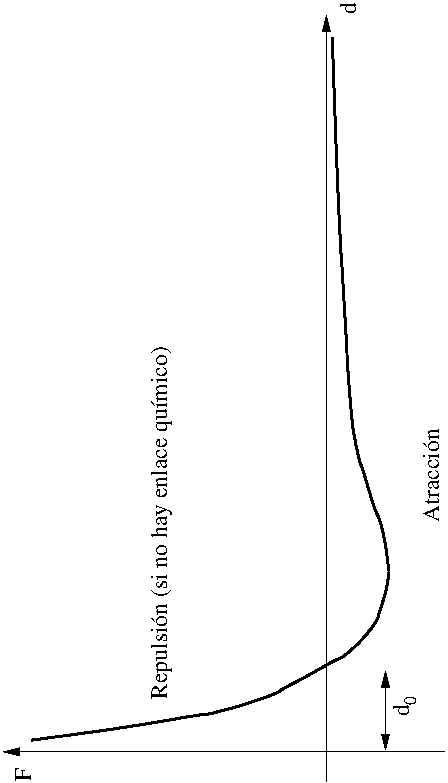
\includegraphics[scale=1,angle=270]{TeX_files/chapter01-Introduccion/fuerzas_molec.pdf}
	\caption{Fuerzas intermoleculares}
	
\end{figure}

En $d_0$, se produce un equilibrio estable.

Para la mayoria de las mol\'eculas, $d_0$ es del orden de  $3-4\cdot10^{-10}$ metros.

Para l\'{\i}quidos, la distancia entre mol\'eculas es, aproximadamente, $d_0$. P.e., para el agua:

$$
\rho \approx 1000 \, \textrm{Kg}/\textrm{m}^3
$$
$$
\textrm{Peso molecular} \approx 0.018 \, \textrm{Kg}/\textrm{mol} \Rightarrow
m = 3.0 \cdot 10^{-26} \, \textrm{Kg}/\textrm{molecula}
$$
$$
V_m = \frac{3.0 \cdot 10^{-26} \, \textrm{Kg}/\textrm{molecula}}{1000 \, \textrm{Kg}/\textrm{m}^3}
=3.0 \cdot 10^{-29} \, \textrm{m}^3
$$
$$
V_m = \frac{4}{3} \pi R^3 \Rightarrow R \approx 1.9 \cdot 10^{-10} \, \textrm{m}
$$

Para los gases, la distancia es mucho mayor (Ejercicio: calcular $d$ para el aire).

As\'{\i}, las fuerzas entre las mol\'eculas de un gas son atractivas y muy d\'ebiles. Estas mol\'eculas
flotan por el espacio sin pr\'acticamente ninguna interacci\'on excepto las colisiones.

\section{Hipótesis del medio continuo}

Todos los materiales est\'an formados por mol\'eculas. Las propiedades del material no estan distribuidas
uniformemente. Si la escala de observaci\'on es lo bastante peque\~na, la composici\'on molecular del material
debe tenerse en cuenta (hablamos entonces de {\em Mec\'anica Estad\'{\i}stica}).

Sin embargo, en {\em Mec\'anica de Fluidos}, se habla normalmente de la densidad, la temperatura, la velocidad,
como una \textcolor{red}{distribuci\'on uniforme de estas propiedades}, sin considerar la naturaleza discreta de la materia. Es
normal hablar de "diferenciales de volumen". Sin embargo, estos diferenciales no son los mismos que los usados
en C\'alculo Infinitesimal. Son volumenes finitos, pero

\begin{itemize}
	\item lo suficientemente grandes como para albergar un n\'umero enorme de mol\'eculas, de forma que las fluctuaciones en las propiedades se anulen entre s\'{\i}, y
	\item lo suficientemente peque\~nos como para que la propiedad pueda ser considerada \em{local}.
\end{itemize}

Batchelor \cite{Batchelor1997} lo describe muy bien con una figura parecida a esta:
\begin{center}
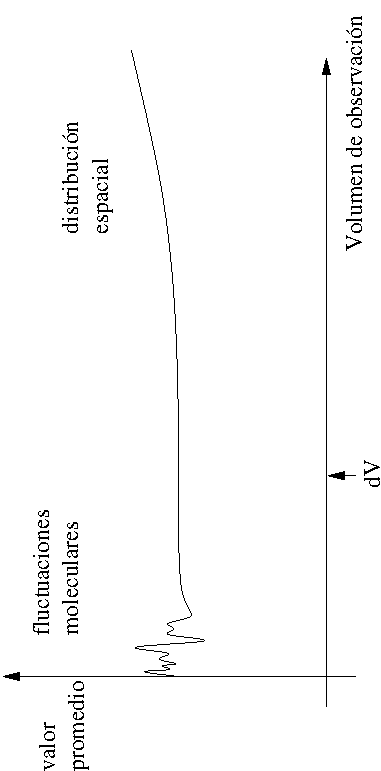
\includegraphics[scale=1,angle=270]{TeX_files/chapter01-Introduccion/difer_vol.pdf}
\end{center}

\section{Propiedades de los fluidos}
\begin{itemize}
	\item \textbf{Propiedades mec\'anicas}
	\begin{itemize}
		\item{\textcolor{red}{densidad - volumen espec\'{\i}fico}}
		$$
		\rho = \frac{m}{V} \qquad ; \qquad \left[\rho\right] = \frac{\textrm{Kg}}{\textrm{m}^3}
		$$
		$$
		v = \frac{1}{\rho} = \frac{V}{m} \qquad ; \qquad \left[v\right] = \frac{\textrm{m}^3}{\textrm{Kg}}
		$$
		\item{\textcolor{red}{M\'odulo de elasticidad} (isot\'ermico)}
		$$
		\beta_T = -v \left(\deriv{p}{v}\right)_T = \rho \left(\deriv{p}{\rho}\right)_T \qquad ; \qquad \left[\beta_T\right] = \textrm{Pa}
		$$
		
		Dado que, \textit{para un gas ideal a temperatura constante}, $\rho \propto p$, tenemos que $\beta_T = p$.
		
		Para una variaci\'on de presi\'on $\Delta p$, la variaci\'on relativa de densidad se puede calcular mediante
		
		$$
		\frac{\Delta \rho}{\rho} = \frac{\Delta p}{\beta_T}
		$$
		
		
		\begin{quotation}
			\textbf{Criterio de compresibilidad} : Todos los fluidos son compresibles, en mayor o menor grado.
			Es importante saber en qu\'e condiciones  un fluido podr\'a ser considerado compresible y cu\'ando no. Supongamos que es considerado compresible si $\frac{\Delta \rho}{\rho} \leq 0.01$. Entonces,
			$$
			\frac{\Delta p}{\beta_T} \lessapprox 0.01.
			$$
			
			Como veremos m\'as adelante, se puede relacionar $\Delta p$ con la velocidad de flujo,
			$$
			\Delta p \sim \frac{1}{2} \rho u^2,
			$$
			de forma que un fluido con velocidad $u$ se puede considerar incompresible si
			$$
			\frac{\rho u^2}{\beta_T} \lessapprox 0.02.
			$$
			
			Como ejemplo, consideremos el aire a presi\'on atmosf\'erica, $ \beta_T = p = 10^5 \,\textrm{Pa}$,
			$\rho \approx 1.2 \,\frac{\textrm{Kg}}{\textrm{m}^3}$.
			
			$$ u^2 \lessapprox \frac{0.02 \beta_T}{\rho} = \frac{0.02 \cdot 10^5}{1.2} = 1.66 \cdot 10^3 \textrm{m}^2/\textrm{s}^2$$
			$$ \Rightarrow u \approx 40 \, \textrm{m/s} $$
			
			\subsection*{Ejercicio} 
			Para el agua, a $20^\circ C$ y presi\'on atmosf\'erica, $\beta_T \approx \unit[2.2\times 10^9]{Pa}$
			y $\rho \approx \unit[1000]{Kg/m^3}$.
			Calcular para qu\'e orden de magnitud de velocidad de flujo el agua debe empezar a considerarse compresible.
		\end{quotation}
		
		\item{\textcolor{red}{Viscosidad}}
		
		Si un fluido fluye en la direcci\'on $x$, de forma ordenada, por capas, aumentando la velocidad en la direcci\'on
		$z$, como muestra la figura,
		
		\begin{center}
			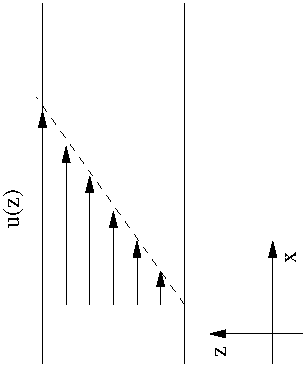
\includegraphics[scale=1,angle=270]{TeX_files/chapter01-Introduccion/u_z.pdf}
		\end{center}
		
		se produce un intercambio de cantidad de movimiento entre capas que tiende a frenar las m\'as r\'apidas y acelerar las m\'as lentas. Es decir, se produce un \textit{esfuerzo tangencial}. En muchos casos, \'este esfuerzo es proporcional al gradiente de velocidades, y a la constante de proporcionalidad se le denomina \textit{\textcolor{red}{viscosidad din\'amica}}, $\mu$. Ésta es la conocida como \textbf{Ley de Newton de la viscosidad}.
		
		\begin{equation}
			\tau = \mu \dparc{u}{z} \qquad ; \qquad \left[\mu\right] = \textrm{Pa}\cdot\textrm{s}
		\end{equation}
		
		
		La \textit{\textcolor{red}{viscosidad cinem\'atica}} se define como
		$$
		\nu = \frac{\mu}{\rho} \qquad ; \qquad \left[\nu\right] = \frac{\textrm{m}^2}{s}
		$$
		
		Ampliaremos el concepto de viscosidad en el tema siguiente.
		
	\end{itemize}
	\item {\textbf{Propiedades termodin\'amicas}}
	
	\textcolor{red}{entalp\'{\i}a}
	$$ h = u + \frac{p}{\rho} = u + p v \qquad ; \qquad \left[h\right] = \left[u\right] = \frac{\textrm{J}}{\textrm{Kg}},
	$$
	
	\textcolor{red}{calor espec\'{\i}fico}
	\begin{eqnarray*}
		c_v = \left(\dparc{q}{T}\right)_v = \dparc{u}{T} & \textrm{a volumen constante} \\
		c_p = \left(\dparc{q}{T}\right)_p = \dparc{h}{T} & \textrm{a presi\'on constante}
	\end{eqnarray*}
	$$
	\left[ c_p \right] = \left[ c_v \right] = \frac{\textrm{J}}{\textrm{Kg}\cdot\textrm{K}}
	$$
	
	La relaci\'on entre ambos coeficientes es:
	$$
	c_p = c_v + \dparc{p v}{T}
	$$
	
	Para un gas perfecto,
	$$ pv = R^\prime T  \Rightarrow \dparc{pv}{T} = R^\prime $$
	$$ \Rightarrow c_p = c_v + R^\prime $$,
	donde $R^\prime = \frac{R}{M}$.
	
	El cociente entre los dos coeficientes se denomina \textit{\textcolor{red}{exponente adiab\'atico}},
	$$
	\gamma = \frac{c_p}{c_v}.
	$$
	
	\textcolor{red}{coeficiente de expansi\'on t\'ermica}
	
	Normalmente,  $\uparrow T \Rightarrow \uparrow v \, (\Rightarrow \downarrow \rho)$.
	
	$$
	\alpha = \frac{1}{v}\deriv{v}{T} = - \frac{1}{\rho} \deriv{\rho}{T} \qquad; \qquad \left[ \alpha \right] = \textrm{K}^{-1}
	$$
	
	Para agua en condiciones normales, $\alpha \approx 1.5\cdot10^{-4} \,\textrm{K}^{-1}$.
	
	Consideremos un gas perfecto, a presi\'on constante,
	$$
	\alpha_p = -\frac{1}{\rho}\left( \dparc{\rho}{T}\right)_p,
	$$
	como $\rho = \frac{p}{R^\prime T}$,
	$$\left(\dparc{\rho}{T}\right)_p = -\frac{p}{R^\prime T^2} \qquad \Rightarrow \alpha_p = \frac{1}{T}$$	
\end{itemize}

\section{Fuerzas sobre fluidos}
\subsection{Fuerzas de superficie}

Act\'uan sobre el contorno de un  volumen determinado de fluido.

Se crean por contacto bien del mismo fluido, un fluido diferente o un s\'olido.

Dada una superficie $\delta \vec S$, y una fuerza superficial $\delta \vec F$ actuando sobre ella, \'esta se
puede descomponer en una componente normal y una componente tangencial.

\begin{center}
	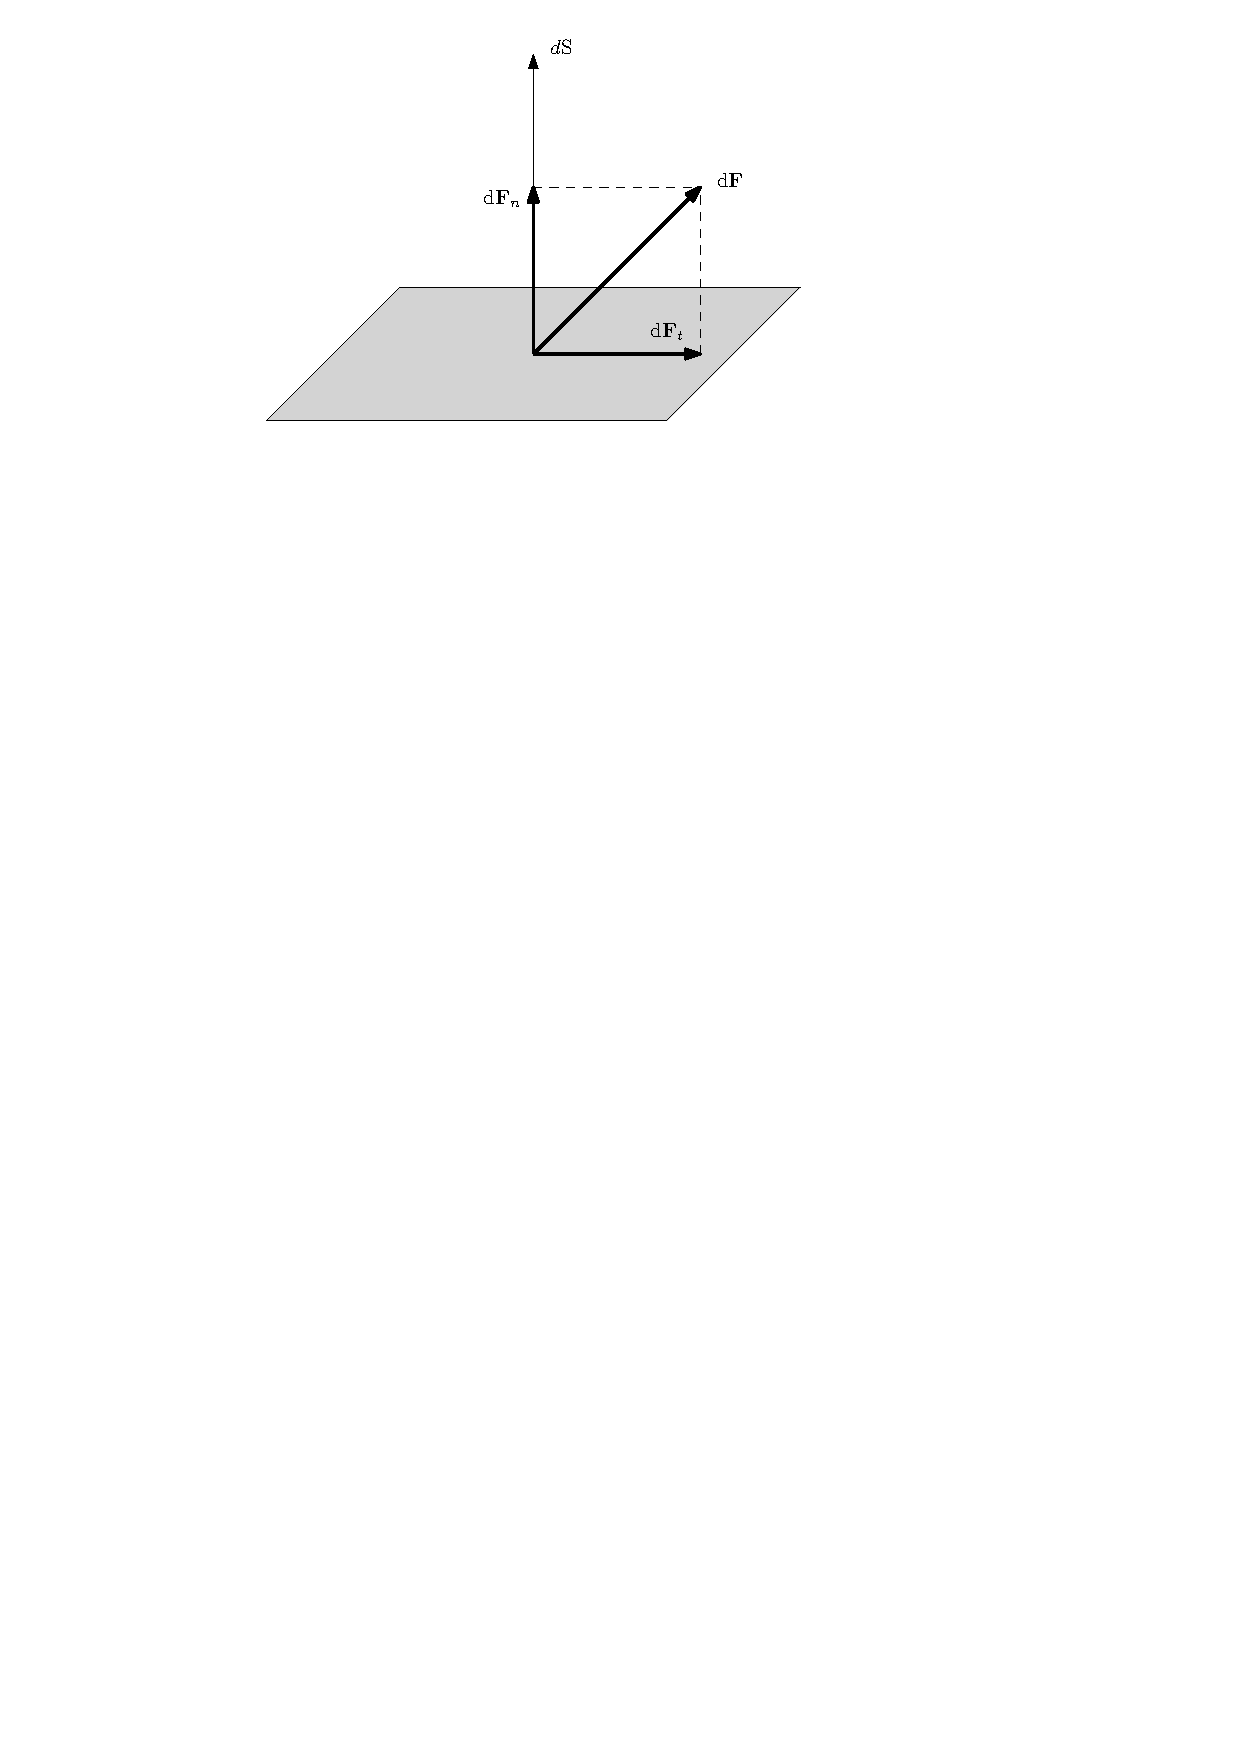
\includegraphics{TeX_files/chapter01-Introduccion/dS.pdf}
\end{center}

Definici\'on de tensi\'on o esfuerzo:

%\begin{center}
	\begin{tabular}{ll}
		\textcolor{blue}{esfuerzo normal} : & \begin{minipage}{10cm}$$\sigma = \lim_{\delta \vec S \rightarrow 0} \frac{\delta \vec F_n}{\delta \vec S}$$\end{minipage} \\
		\textcolor{blue}{esfuerzo tangencial} : & \begin{minipage}{10cm}$$\tau = \lim_{\delta \vec S \rightarrow 0} \frac{\delta \vec F_t}{\delta \vec S}$$ \end{minipage}\\
	\end{tabular}
%\end{center}

\begin{description}
	\item[$\sigma_i$ :] esfuerzo normal aplicado sobre una superficie normal al eje $i$ (y, por lo tanto, paralelo al eje $i$)
	\item[$\tau_{ij}$ :] esfuerzo tangencial aplicado sobre una superficie normal al eje $i$, y en la direcci\'on del eje $j$
\end{description} 

\begin{center}
%	\tikzstyle{isometric}=[x={(0.710cm,-0.410cm)},y={(0cm,0.820cm)},z={(-0.710cm,-0.410cm)}]
\tikzstyle{dimetric} =[x={(0.935cm,-0.118cm)},y={(0cm,0.943cm)},z={(-0.354cm,-0.312cm)}]
\tikzstyle{dimetric2}=[x={(0.935cm,-0.118cm)},z={(0cm,0.943cm)},y={(+0.354cm,+0.312cm)}]
\tikzstyle{trimetric}=[x={(-0.926cm,0.207cm)},y={(0cm,0.837cm)},z={(0.378cm,0.507cm)}]

\begin{tikzpicture}[trimetric]
	\coordinate (O) at (0,0,0);
	\draw[-stealth] (0,0,0) -- (6,0,0) node[above]{$x$};
	\draw[-stealth] (0,0,0) -- (0,6,0) node[above]{$y$};
	\draw[-stealth] (0,0,0) -- (0,0,6) node[above]{$z$};
	\draw[fill=gray!30] (0,0,0) -- (0,4,0) -- (0,4,4) -- (0,0,4)-- cycle;	
	\draw (0,0,0) -- (4,0,0) -- (4,4,0) -- (0,4,0)-- cycle;
	\draw (0,0,0) -- (0,0,4) -- (4,0,4) -- (4,0,0)-- cycle;
	\draw[fill=gray!30] (4,0,0) -- (4,4,0) -- (4,4,4) -- (4,0,4)-- cycle;	
	\draw (0,0,4) -- (4,0,4) -- (4,4,4) -- (0,4,4)-- cycle;
	\draw (0,4,0) -- (0,4,4) -- (4,4,4) -- (4,4,0)-- cycle;
%
	\draw[-stealth,thick] (0,2,2) -- (-1,2,2) node[above ]{$\sigma_x$};
	\draw[-stealth,thick] (0,2,2) -- (0,1,2) node[right]{$\tau_{xy}$};
	\draw[-stealth,thick] (0,2,2) -- (0,2,1) node[above=2mm]{$\tau_{xz}$};
%
	\draw[-stealth,thick] (4,2,2) -- (5,2,2) node[left=2mm]
					{$\sigma_x+\frac{\partial \sigma_x}{x} \textrm{d}x$};
	\draw[-stealth,thick] (4,2,2) -- (4,3,2) node[above left]
					{$\tau_{xy}+\frac{\partial \tau_{xy}}{x} \textrm{d}x$};
	\draw[-stealth,thick] (4,2,2) -- (4,2,3) node[right]
					{$\tau_{xz}+\frac{\partial \tau_{xz}}{x} \textrm{d}x$};
\end{tikzpicture}
\tikzstyle{isometric}=[x={(0.710cm,-0.410cm)},y={(0cm,0.820cm)},z={(-0.710cm,-0.410cm)}]
\tikzstyle{dimetric} =[x={(0.935cm,-0.118cm)},y={(0cm,0.943cm)},z={(-0.354cm,-0.312cm)}]
\tikzstyle{dimetric2}=[x={(0.935cm,-0.118cm)},z={(0cm,0.943cm)},y={(+0.354cm,+0.312cm)}]
\tikzstyle{trimetric}=[x={(-0.926cm,0.207cm)},y={(0cm,0.837cm)},z={(0.378cm,0.507cm)}]

\begin{tikzpicture}[trimetric]
	\coordinate (O) at (0,0,0);
	\draw[-stealth] (0,0,0) -- (6,0,0) node[above]{$x$};
	\draw[-stealth] (0,0,0) -- (0,6,0) node[above]{$y$};
	\draw[-stealth] (0,0,0) -- (0,0,6) node[above]{$z$};
	\draw[fill=gray!30] (0,0,0) -- (0,4,0) -- (0,4,4) -- (0,0,4)-- cycle;	
	\draw (0,0,0) -- (4,0,0) -- (4,4,0) -- (0,4,0)-- cycle;
	\draw (0,0,0) -- (0,0,4) -- (4,0,4) -- (4,0,0)-- cycle;
	\draw[fill=gray!30] (4,0,0) -- (4,4,0) -- (4,4,4) -- (4,0,4)-- cycle;	
	\draw (0,0,4) -- (4,0,4) -- (4,4,4) -- (0,4,4)-- cycle;
	\draw (0,4,0) -- (0,4,4) -- (4,4,4) -- (4,4,0)-- cycle;
%
	\draw[-stealth,thick] (0,2,2) -- (-1,2,2) node[above ]{$\sigma_x$};
	\draw[-stealth,thick] (0,2,2) -- (0,1,2) node[right]{$\tau_{xy}$};
	\draw[-stealth,thick] (0,2,2) -- (0,2,1) node[above=2mm]{$\tau_{xz}$};
%
	\draw[-stealth,thick] (4,2,2) -- (5,2,2) node[left=2mm]
					{$\sigma_x+\frac{\partial \sigma_x}{x} \textrm{d}x$};
	\draw[-stealth,thick] (4,2,2) -- (4,3,2) node[above left]
					{$\tau_{xy}+\frac{\partial \tau_{xy}}{x} \textrm{d}x$};
	\draw[-stealth,thick] (4,2,2) -- (4,2,3) node[right]
					{$\tau_{xz}+\frac{\partial \tau_{xz}}{x} \textrm{d}x$};
\end{tikzpicture}
\end{center}

Sobre el volumen $\text{d} V$ act\'ua una fuerza, debida a los esfuerzos superficiales cuya componente $x$ es
\begin{multline}
	\dif F_x = -\sigma_x  \dif y \dif z + \left(\sigma_x + \dparc{\sigma_x}{x} \dif x\right) \dif y \dif z - \tau_{yx} \dif x \dif z + \left(\tau_{yx} + \dparc{\tau_{yx}}{y}\right) \dif x \dif z \\
	- \tau_{zx} \dif x \dif y + \left(\tau_{zx} + \dparc{\tau_{zx}}{z}\right) \dif x \dif y
	= \dparc{\sigma_x}{x} \dif x \dif y \dif z + \dparc{\tau_{yx}}{y} \dif x \dif y \dif z + \dparc{\tau_{zx}}{z}
	\dif x \dif y \dif z
\end{multline}
De la misma forma:
\begin{eqnarray}
	\dif F_y = \dparc{\sigma_y}{y} \dif x \dif y \dif z + \dparc{\tau_{xy}}{x} \dif x \dif y \dif z + \dparc{\tau_{zy}}{z} \dif x \dif y \dif z \\
	\dif F_z = \dparc{\sigma_z}{z} \dif x \dif y \dif z + \dparc{\tau_{xz}}{x} \dif x \dif y \dif z + \dparc{\tau_{yz}}{y} \dif x \dif y \dif z
\end{eqnarray}

La fuerza por unidad de volumen, debida a los esfuerzos superficiales es entonces
\begin{eqnarray*}
	\vec f = \deriv{\vec F}{V} = \left( \dparc{\sigma_x}{x} + \dparc{\tau_{yx}}{y} + \dparc{\tau_{zx}}{z}\right) \vec \imath \\
	+ \left( \dparc{\tau_{xy}}{x} + \dparc{\sigma_y}{y} +  \dparc{\tau_{zy}}{z} \right) \vec \jmath \\
	+ \left( \dparc{\tau_{xz}}{x}  +  \dparc{\tau_{yz}}{y} + \dparc{\sigma_z}{z} \right) \vec k
\end{eqnarray*}
que se expresa de forma abreviada como
\begin{equation}
	 \vec f = \vec \nabla \vec {\vec \tau}
\end{equation}
donde $\vec {\vec \tau}$ es el \textcolor{red}{tensor de tensiones} (stress tensor)
\begin{equation}
	\vec{\vec{\tau}} =
	\left(
	\begin{array}{ccc}
		\sigma_x & \tau_{xy} & \tau_{xz} \\
		\tau_{yx} & \sigma_y & \tau_{yz} \\
		\tau_{zx} & \tau_{zy} & \sigma_z
	\end{array}\right)
\end{equation}

\subsection{Fuerzas m\'asicas}
Act\'uan a distancia

Son debidas a campos de fuerza (gravitacional, electromagn\'etico, \ldots)

Fluido el\'ectricamente cargado : plasma
\begin{itemize}
	\item Electrohidrodin\'amica
	\item Magnetohidrodin\'amica
\end{itemize}

Caso m\'as com\'un: s\'olo campo gravitacional
$$\vec f_g = \rho \vec g$$

\subsection{Fuerzas lineales (tensi\'on superficial)}
En la interfase de separaci\'on entre dos l\'iquidos reside una cantidad de energ\'{\i}a, correspondiente
a la interacci\'on entre moleculas muy pr\'oximas a la superficie de separaci\'on

Esta energ\'{\i}a es proporcional al \'area de la interfase.
\begin{equation}
	 E_s = \sigma S
\end{equation} 

El par\'ametro $\sigma$ recibe el nombre de \textcolor{blue}{tensi\'on superficial} y tiene unidades de fuerza por
unidad de longitud. Esta fuerza es tangente a la superficie, y normal a la l\'{\i}nea de aplicaci\'on.

El valor de $\sigma$ depende de la naturaleza de los materiales que separa la interfase y de su estado termodin\'amico.

P.e. para la interfase entre agua y aire a $20^\circ C$, $\sigma~=~72.8\cdot10^{-3}~\text{N/m}$


\begin{center}
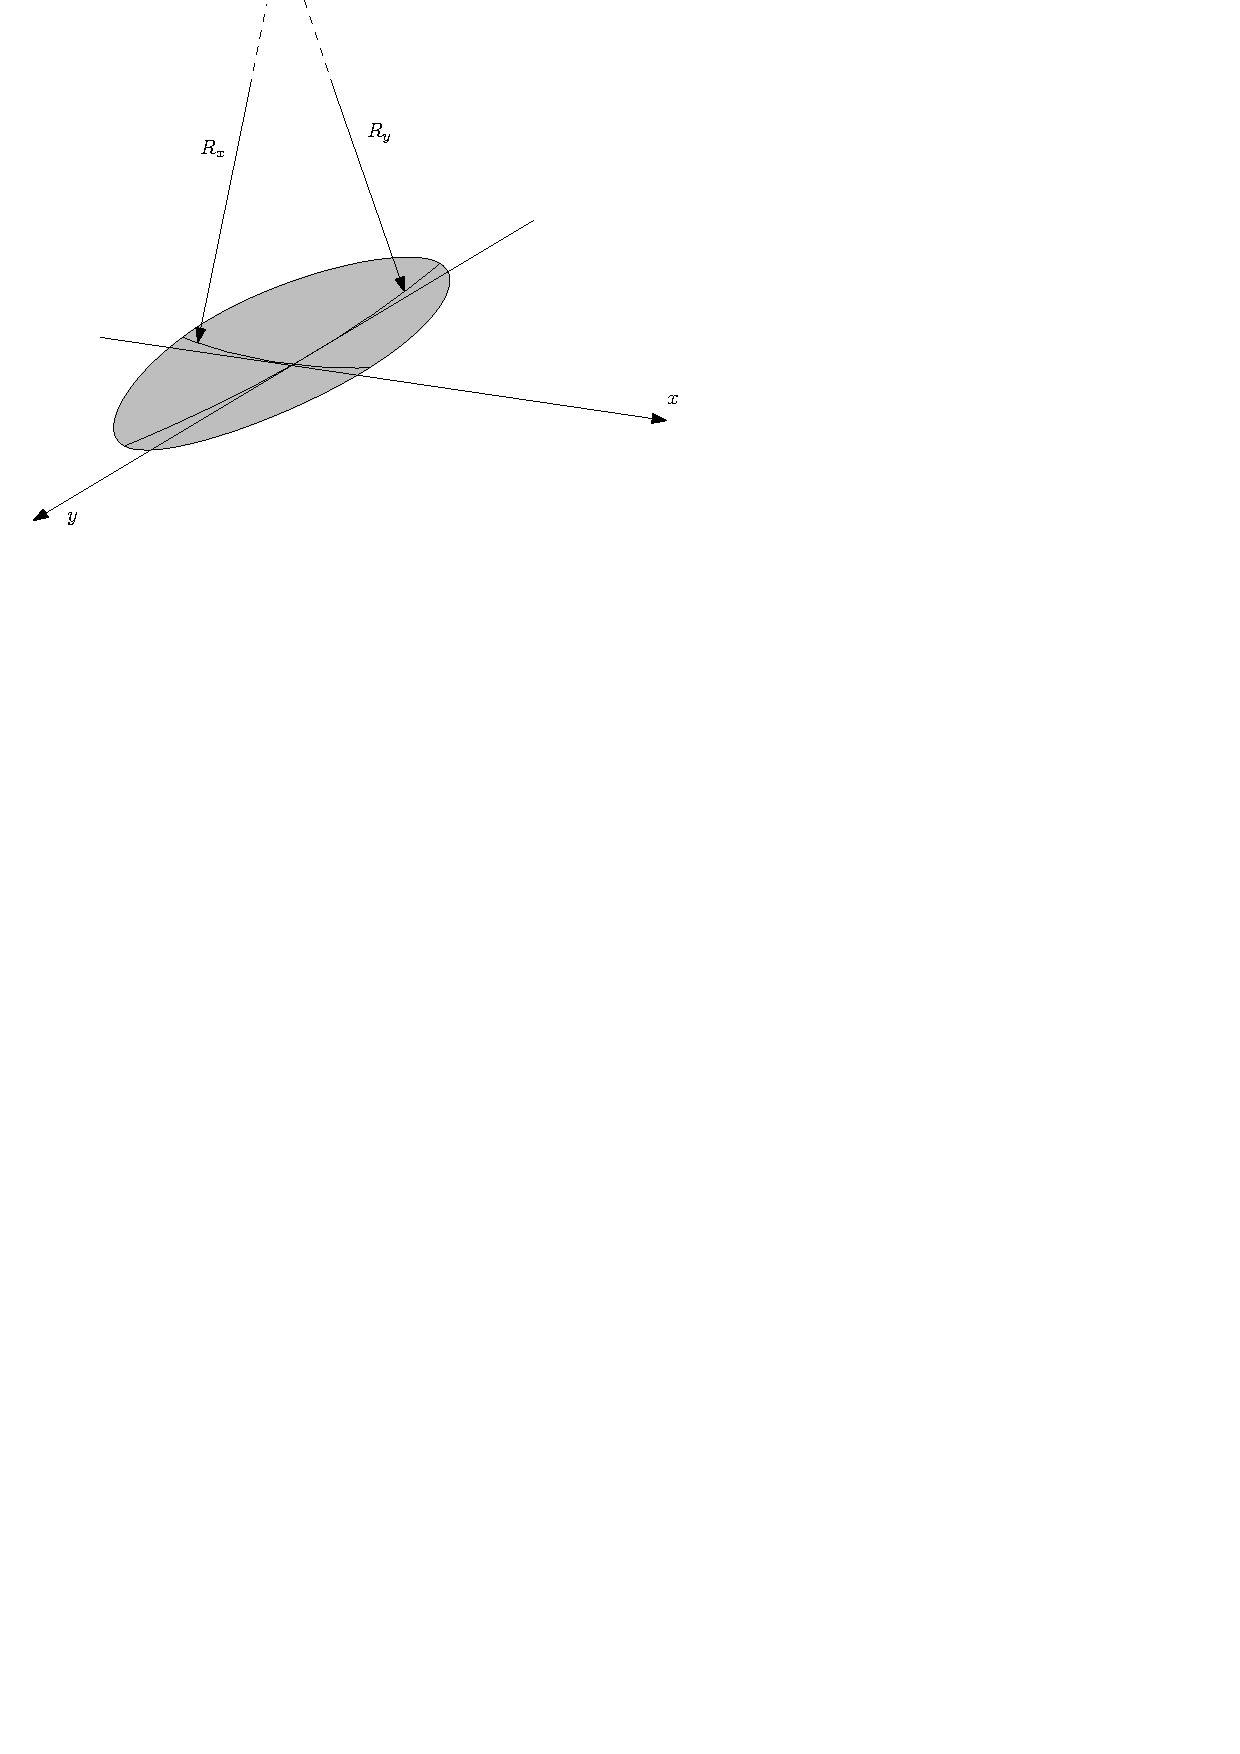
\includegraphics{TeX_files/chapter01-Introduccion/YoungLaplace}
\end{center}
Se puede demostrar (ver \cite{Batchelor1997}) que la tensi\'on provocada en la superfice es equivalente a una diferencia
de presi\'on, como indica la \href{https://es.wikipedia.org/wiki/Ley_de_Laplace}{\textbf{ley de Young-Laplace}}
\begin{equation}
	\Delta p = \sigma\left(\frac{1}{R_x}+\frac{1}{R_y}\right)
\end{equation}


Si los dos radios de curvatura son iguales, ($R_x=R_y=R$, casquete esférico), esta expresión se reduce a 
 
\begin{equation}
	\Delta p = \frac{2\sigma}{R}
\end{equation}

Consideramos el caso de tres fluidos (p.e. una gota de aceite en una superficie de agua)
\begin{center}
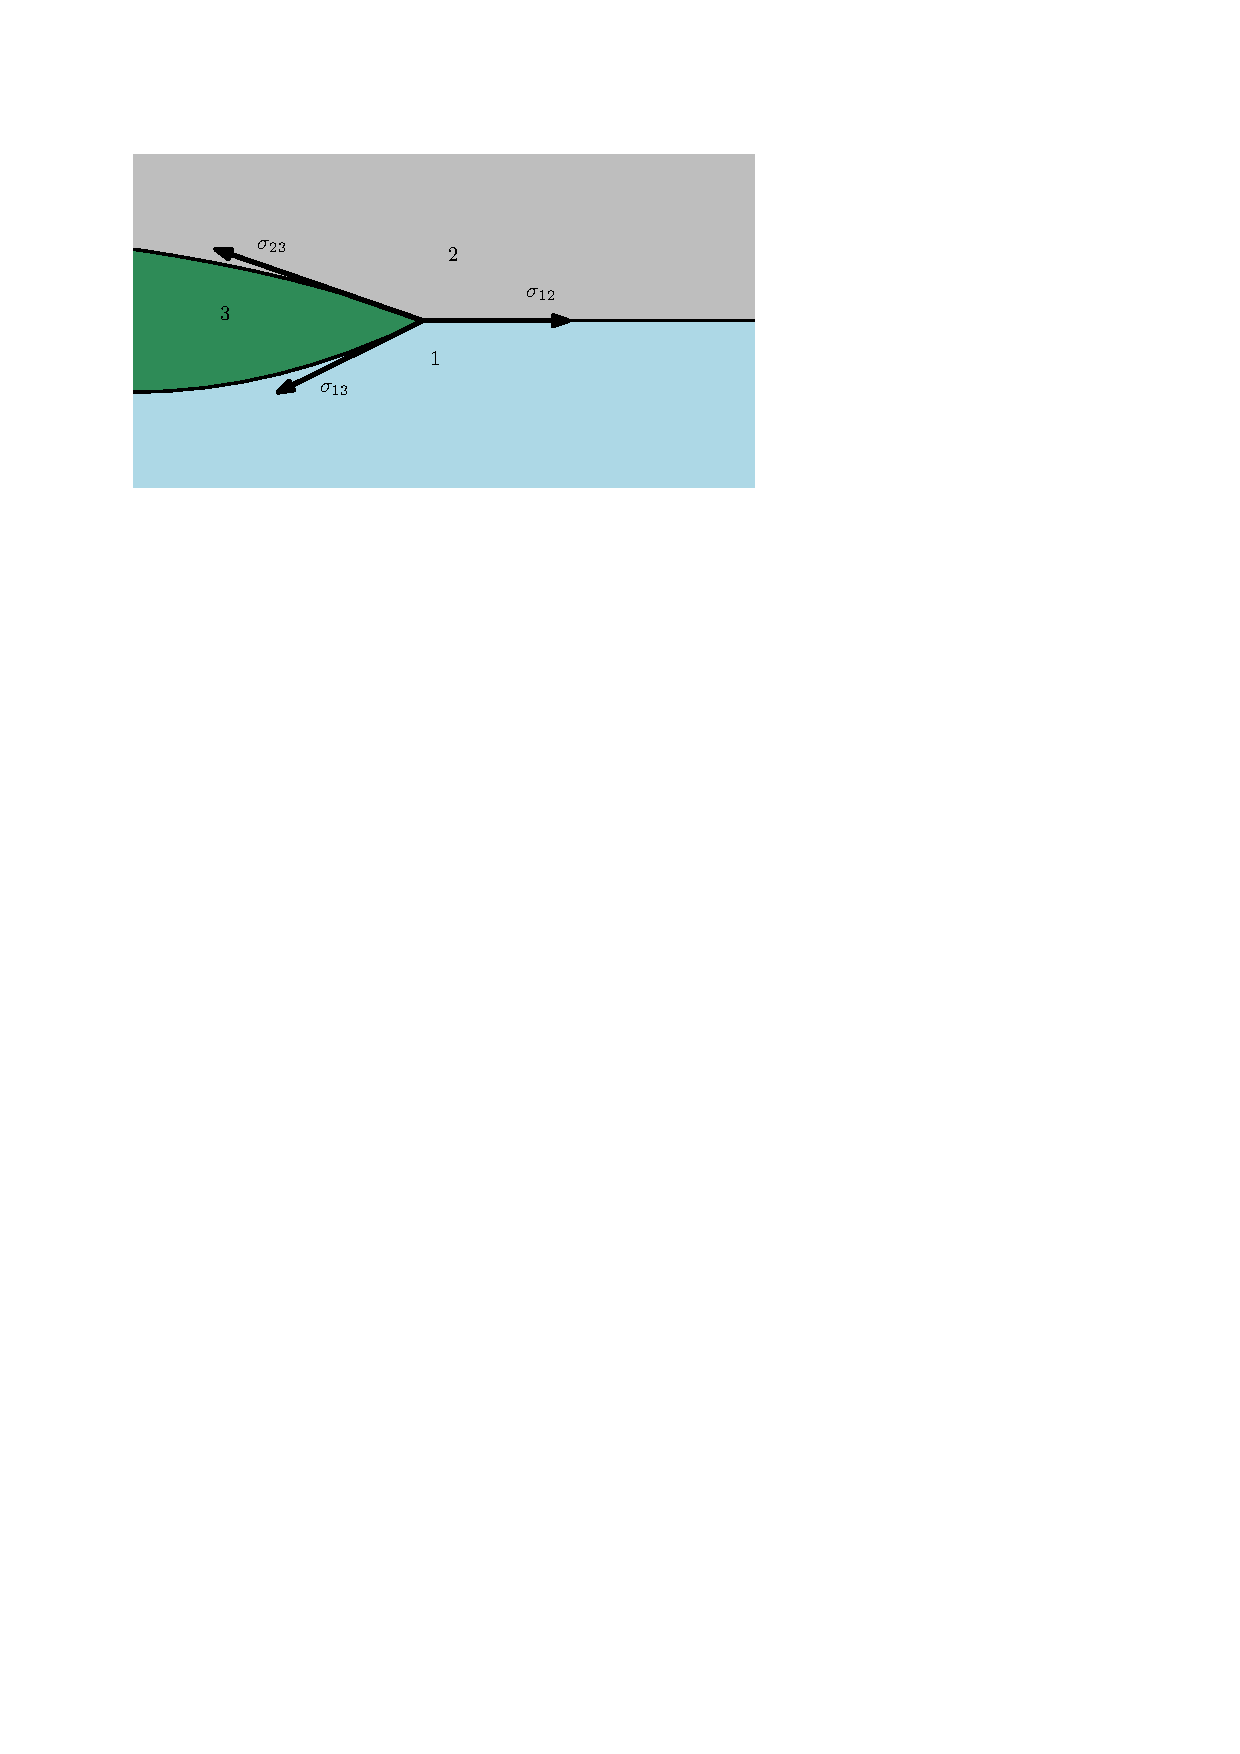
\includegraphics{TeX_files/chapter01-Introduccion/tresFluidos}
\end{center}
Si el m\'odulo de una de las tensiones es mayor que la suma de los m\'odulos de las otras dos, este sistema nunca
puede llegar al equilibrio, y el fluido se expandir\'a de forma indefinida hasta llegar al equilibrio, o tener
un grosor de tama\~no molecular.

Si uno de los materiales es un s\'olido,
\begin{center}
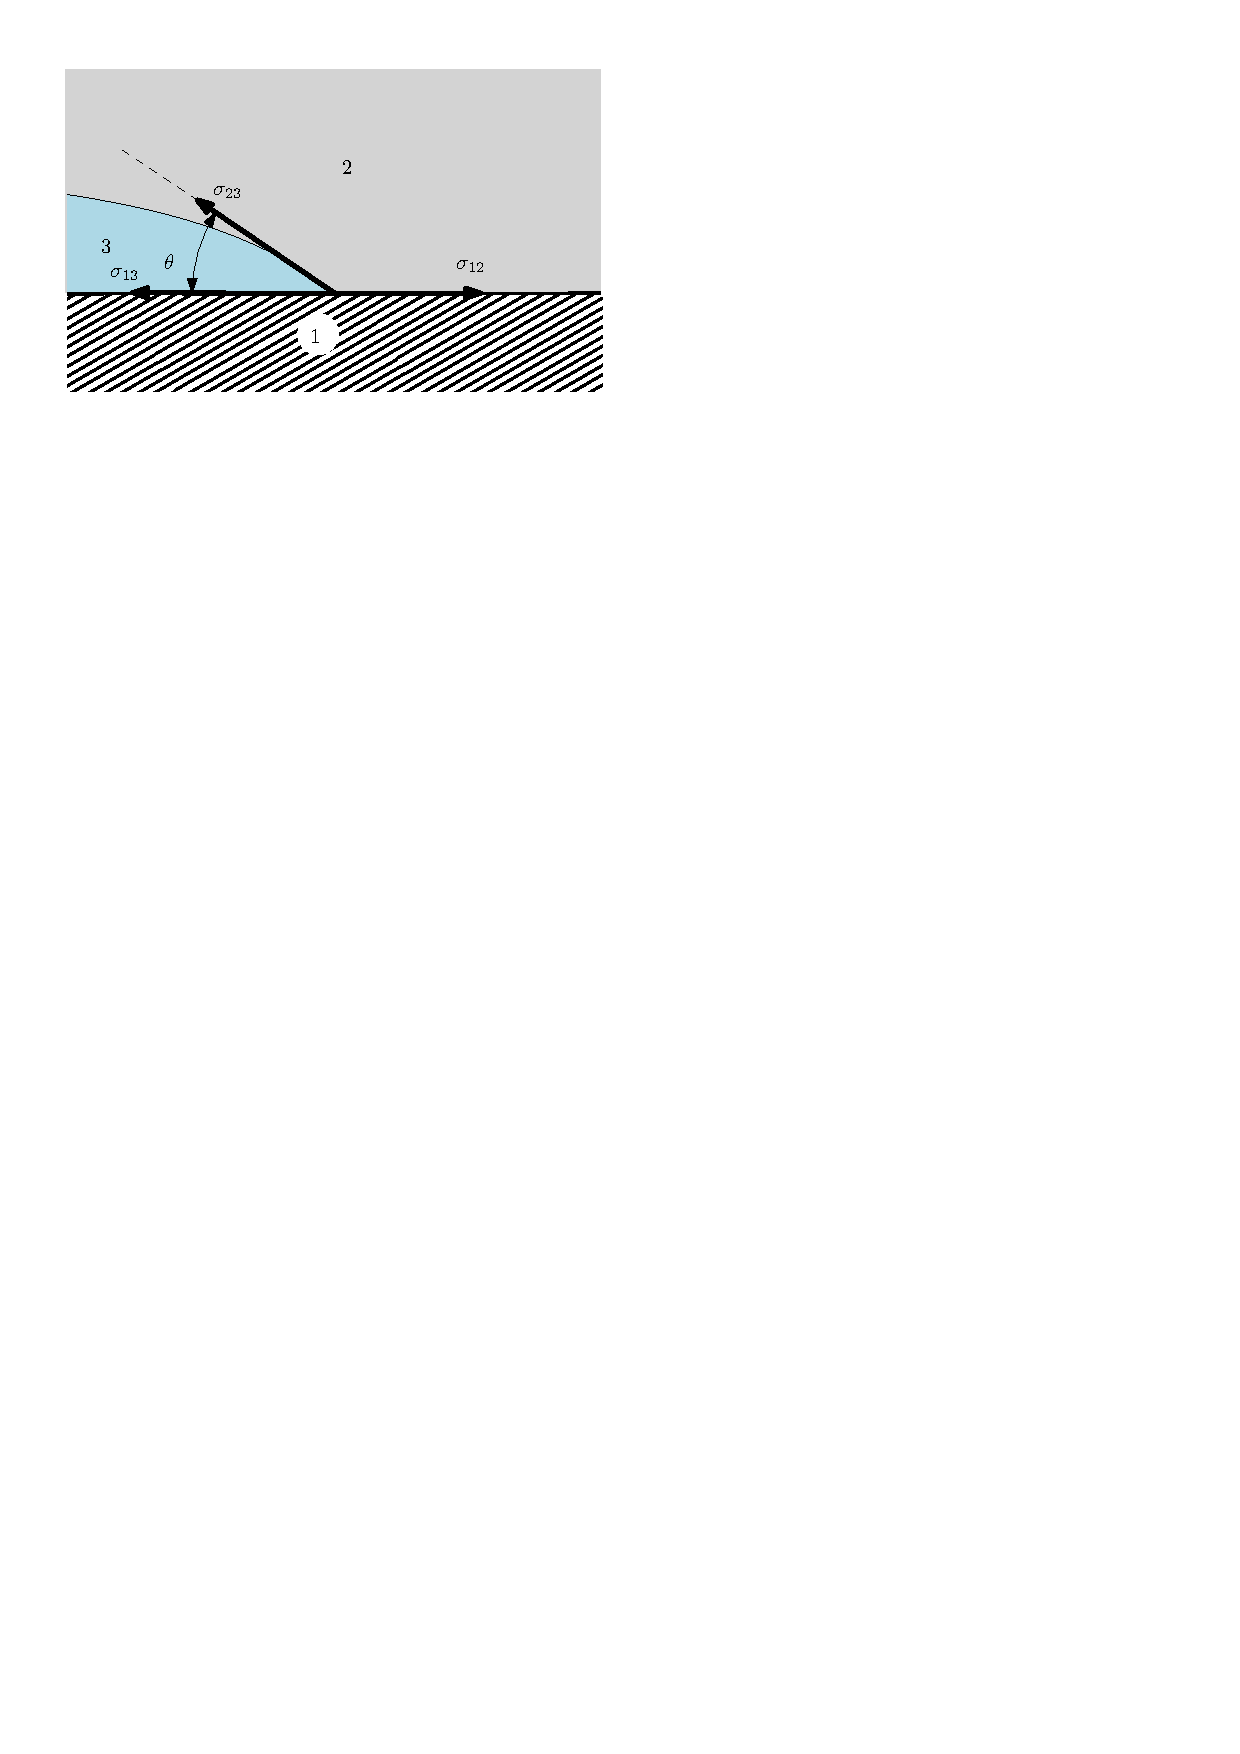
\includegraphics{TeX_files/chapter01-Introduccion/dosysolido}
\end{center}
se llega al equilibrio para
$$ \sigma_{12} = \sigma_{31} + \sigma_{23} \cos{\theta}$$
Se considera que cuanto menor es $\theta$, m\'as "moja" el fluido sobre la superficie del s\'olido.

\subsection*{Ejemplo:}
L\'{\i}quido en contacto con pared plana vertical
\begin{center}
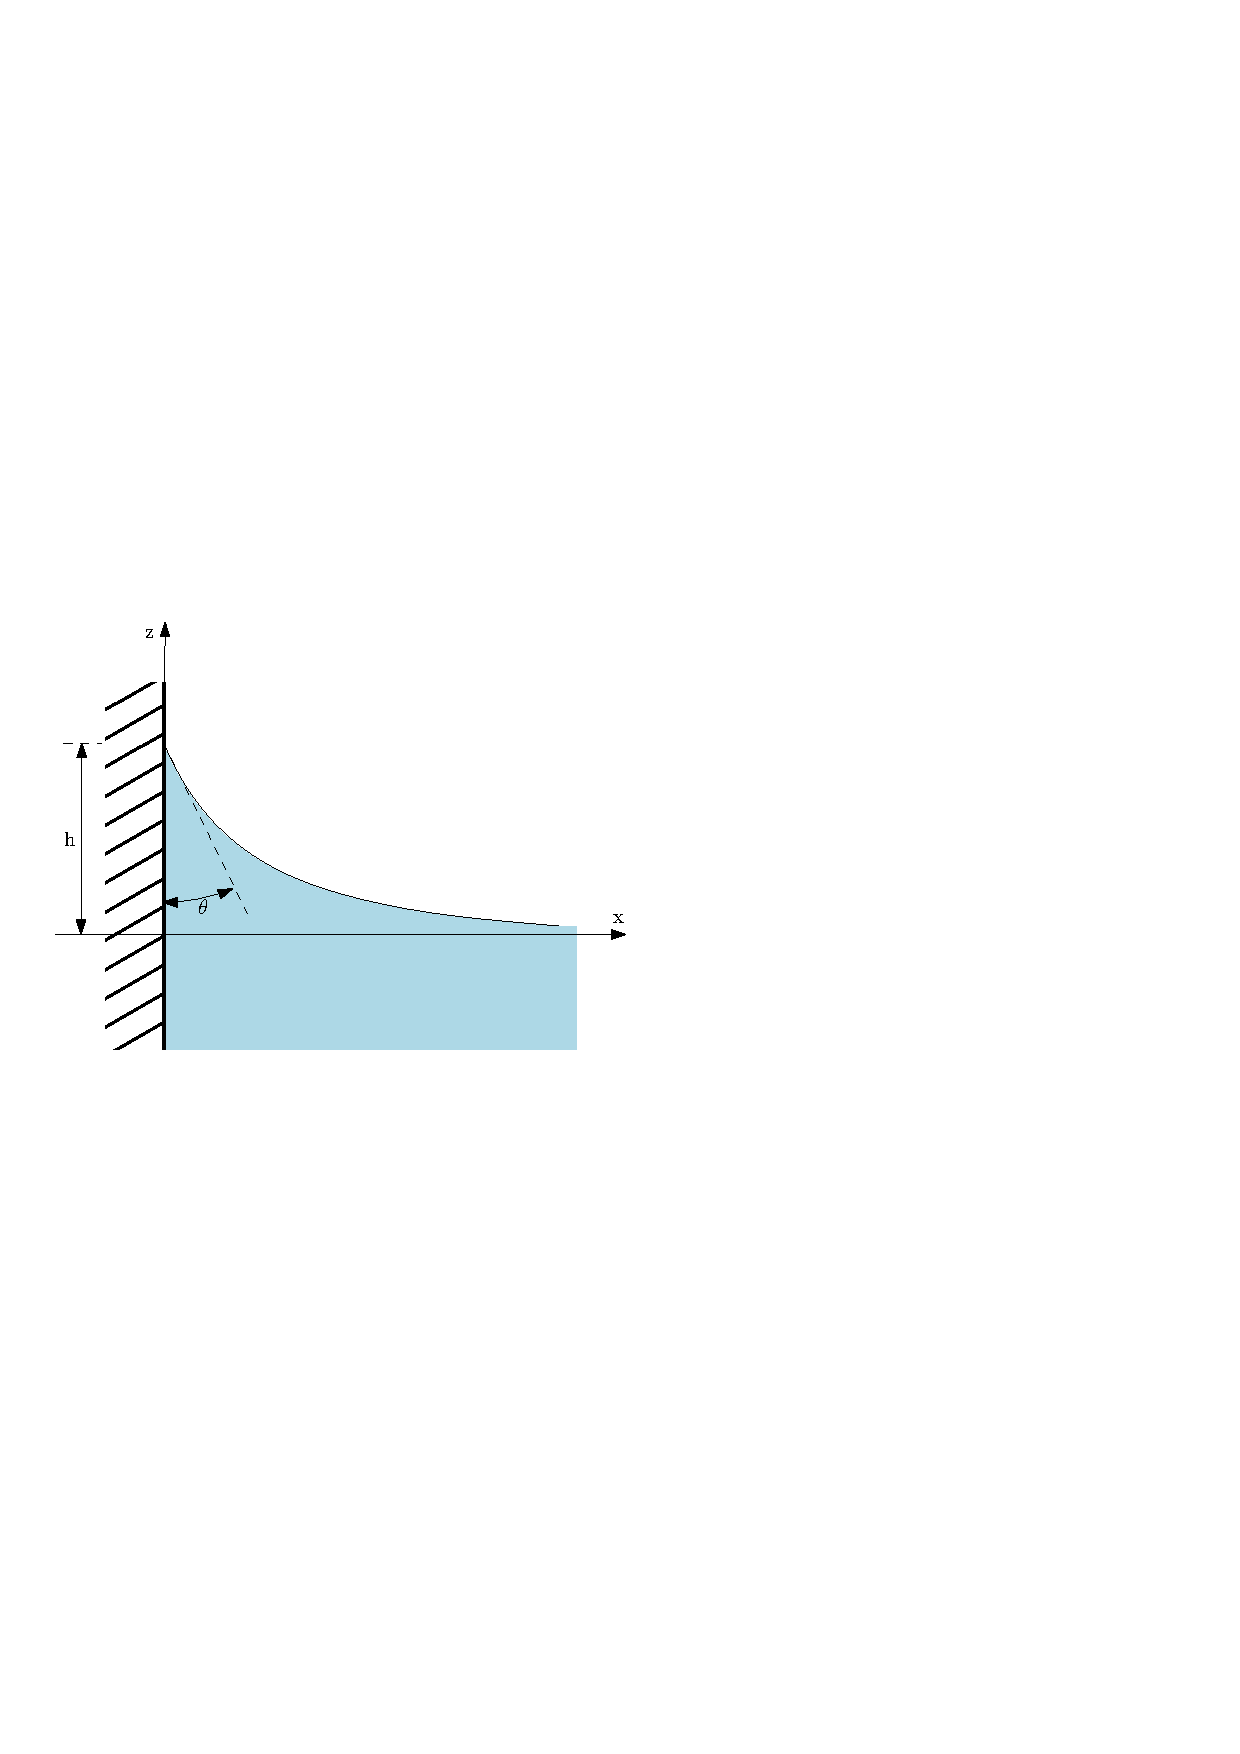
\includegraphics{TeX_files/chapter01-Introduccion/pared.pdf}
\end{center}
Forma de la interficie: $z=\zeta(x)$

En un cierto punto de la interficie, la tensi\'on superficial tiene que ser tal que compense la presi\'on de la columna de fluido. Como veremos m\'as adelante, esta es $\rho g z$, de forma que
$$
\rho g z = \sigma \frac{1}{R_1}
$$
$$
\rho g \zeta = \sigma \frac{\zeta''}{\left( 1 + \zeta'^2\right)^\frac{3}{2}}
$$
Integrando se obtiene
$$
\frac{1}{2}\frac{\rho g}{\sigma}\zeta^2 + \frac{1}{\left(1+\zeta'^2\right)^\frac{1}{2}} = K
$$
Muy lejos de la pared, se cumple que $\zeta=\zeta'=0$, de forma que $K = 1$

Por otro lado, en $x=0$, se tiene (ver figura) $\zeta=h$ y $\zeta'=-\frac{1}{\tan \theta}$, de forma que
$$
h = d \sqrt{2\left(1-\sin \theta \right)}
$$
donde $d^2=\frac{\sigma}{\rho g}$.
\chapter{Hidrostática}

\section{Ecuación fundamental de la fluidostática}

\textbf{Fluido en reposo}: No hay esfuerzos tangenciales, y la única
fuerza superficial es la presión.

Equilibrio estático: 

\begin{equation}
\vec{f}_{m}-\vec{\nabla}p=0
\end{equation}


Según el calculo diferencial, 
\[
\vec{\nabla}\times\left(\vec{\nabla}\phi\right)=0\quad\forall\phi\text{ escalar}
\]

\[
\Rightarrow\vec{\nabla}\times\vec{f_{m}}=0.
\]
 $\Rightarrow\vec{f}_{m}$ ha de ser un \emph{campo conservativo}.

\[
\dif p=\vec{f}_{m}\cdot\dif\vec{r}
\]
 Integrando sobre un determinado camino, 
\[
p\left(\vec{r}\right)=p\left(\vec{r}_{0}\right)+\int_{\vec{r}_{0}}^{\vec{r}}\vec{f}_{m}\cdot\dif\vec{r}
\]
 Nos permite calcular la presión en cualquier punto $\vec{r}$ conociendo
el valor en un punto de referencia $\vec{r}_{0}$ y el campo de fuerzas
$\vec{f}_{m}$.

Si $\vec{f}_{m}$ es conservativo 
\[
\vec{f}_{m}=-\rho\vec{\nabla}U
\]
 y, entonces, 
\[
\vec{\nabla}p=-\rho\vec{\nabla}U
\]

Si $\rho$ varia de forma arbitraria, no existen soluciones para la
ecuación , y no es posible llegar al equilibrio, $\rightarrow$ \textcolor{blue}{corrientes
convectivas}

La ecuación sólo admite soluciones cuando $\rho$ es únicamente función
de la presión, o bien es constante (fluido incompresible). 
\[
p+\rho U=cte
\]

$\rightarrow$ \textcolor{blue}{Principio de Pascal}

Hidrostática en el campo de la gravedad

\[
\vec{f}_{m}=\rho\vec{g},
\]
 con 
\[
\vec{g}=-g\vec{k}\qquad\text{donde }g=9.81\,\frac{\textrm{m}}{\textrm{s}^{2}}
\]
 y 
\[
U=gz
\]



Superficies isobáricas (superficies de igual presión), incluida la
superficie libre de los líquidos, horizontales. %

\[
\vec{\nabla}p=-\rho g\vec{k}\Rightarrow\left\{ \begin{aligned}\dparc{p}{x} & =0\\
\dparc{p}{y} & =0\\
\dparc{p}{z} & =-\rho g
\end{aligned}
\right.
\]
%

La presión es únicamente función de la coordenada $z$.

\[
\deriv{p}{z}=-\rho\,g\Rightarrow\,p_{2}-p_{1}
\]

\[
=-\int_{z_{1}}^{z_{2}}\rho\,g\,\dif z
\]
%

\subsection*{Actividad 1:}
\noindent\begin{minipage}[t]{1\columnwidth}%
\begin{itemize}
\item ¿A cuántos metros de columna de agua corresponden la presión atmosférica?
\item Si el aire fuese incompresible, con la densidad que tiene a nivel
del mar, ¿cuál debería ser la altura de la atmósfera para tener la
misma presión?
\end{itemize}
%
\end{minipage}

\section{Presión atmosférica}

La presión atmosférica disminuye con la altura. Dado que el aire es
un gas, su densidad disminuye, en general, cuando disminuye la presión,
por lo que también es menor cuando aumentamos la altura.

Necesitamos información sobre la variación de $\rho$ con $z$, o
bien con $p$.

Opción: aire gas ideal 
\[
\rho=\frac{pM}{RT}\quad\textnormal{con}\,M=28.9\,\textnormal{g/mol}.
\]
 
\begin{equation}
\Rightarrow\,\frac{\dif p}{p}=-\frac{Mg}{RT}\dif z\label{eq:general}
\end{equation}



Sin considerar la variación de $g$ con la altura: 
\begin{itemize}
\item \textcolor{blue}{Atmósfera isoterma:} 
\[
\int_{p_{0}}^{p}\frac{\dif p}{p}=-\int_{0}^{z}\frac{Mg}{RT}\dif z
\]
 
\[
\ln\frac{p}{p_{0}}=-\frac{Mg}{RT}z=-\frac{\rho_{0}g}{p_{0}}z
\]
 
\begin{equation}
\Rightarrow\boxed{p=p_{0}\exp\left(-\frac{\rho_{0}g}{p_{0}}z\right)=p_{0}\exp\left(-\frac{z}{\alpha}\right)}\label{eq:isotermica}
\end{equation}
 donde 
\[
\alpha=\frac{p_{0}}{\rho_{0}g}
\]
\end{itemize}
Valores normales: 
\[
\left.\begin{aligned}\rho_{0} & =1.292\,\text{Kg}/\text{m}^{3}\\
g & =9.80665\,\text{m}/\text{s}^{2}\\
p_{0} & =760\,\text{mmHg}=101328\,\text{Pa}
\end{aligned}
\right\} \rightarrow\alpha=7997.35\,\text{m}\approx8000\,\text{m}
\]



\begin{itemize}
\item \textcolor{blue}{Atmósfera adiabática:} 
\[
\frac{p}{\rho^{\gamma}}=\frac{p_{0}}{\rho_{0}^{\gamma}}\qquad\text{con}\qquad\gamma=\frac{c_{p}}{c_{v}}=1.4\qquad\text{para aire}
\]
\end{itemize}
\[
\dif p=-g\rho\dif z=-\rho_{0}\left(\frac{p}{p_{0}}\right)^{\frac{1}{\gamma}}g\dif z
\]
 
\[
\Rightarrow\frac{\dif p}{p^{\frac{1}{\gamma}}}=-\frac{\rho_{0}}{p_{0}^{\frac{1}{\gamma}}}g\dif z
\]

\[
\int_{p_{0}}^{p}\frac{\dif p}{p^{\frac{1}{\gamma}}}=\int_{0}^{z}-\frac{\rho_{0}}{p_{0}^{\frac{1}{\gamma}}}g\dif z=-\frac{\rho_{0}}{p_{0}^{\frac{1}{\gamma}}}gz
\]


\[
\Rightarrow\frac{1}{-\frac{1}{\gamma}+1}\left.p^{-\frac{1}{\gamma}+1}\right]_{p_{0}}^{p}=-\frac{\rho_{0}}{p_{0}^{\frac{1}{\gamma}}}gz
\]

\[
\Rightarrow\frac{\gamma}{\gamma-1}\left[p^{\frac{\gamma-1}{\gamma}}-p_{0}^{\frac{\gamma-1}{\gamma}}\right]=-\frac{\rho_{0}}{p_{0}^{\frac{1}{\gamma}}}gz
\]

\[
\Rightarrow p^{\frac{\gamma-1}{\gamma}}-p_{0}^{\frac{\gamma-1}{\gamma}}=\frac{1-\gamma}{\gamma}\frac{\rho_{0}}{p_{0}^{\frac{1}{\gamma}}}gz
\]

\begin{equation}
\Rightarrow\boxed{\left(\frac{p}{p_{0}}\right)^{\frac{\gamma-1}{\gamma}}=1+\frac{1-\gamma}{\gamma}\frac{z}{\alpha}}\label{eq:adiabatica}
\end{equation}


\begin{itemize}
\item \textcolor{blue}{Atmósfera estándar:}
\end{itemize}
En realidad, la temperatura media de la atmósfera disminuye de forma
casi lineal con la altura 
\[
T=T_{0}-Bz
\]
 hasta una altura aproximada de 11000 metros (región conocida como
\textit{troposfera}). Los valores de $T_{0}$ (la temperatura a nivel
del mar) y $B$ (\textit{gradiente térmico}) varían no sólo según
el día sino también a lo largo del mismo día. Los valores estándar
usados por convenio son 
\begin{eqnarray*}
T_{0} & = & 15^{\circ}C=288.16\textnormal{K}\\
B & = & 0.0065\textnormal{K/m}
\end{eqnarray*}



\subsection*{Actividad 2:}
Integrar la ecuación (\ref{eq:general}) con esta distribución de
temperatura para obtener 
\begin{equation}
p=p_{0}\left(1-\frac{Bz}{T_{0}}\right)^{\frac{Mg}{RB}}
\end{equation}

El valor del exponente para aire es 
\[
\frac{Mg}{RB}=5.26
\]

Después de la troposfera, la temperatura se mantiene constante hasta
unos 20000 metros para empezar a aumentar de forma gradual.

Hay que tener siempre en cuenta que esta atmósfera estándar es un
valor promediado. 

\section{Fuerza de un fluido estático sobre una superficie}

\subsection{Cálculo de la fuerza}


\begin{center}
\resizebox{0.8\textwidth}{!}{\input{TeX_files/chapter02-Hidrostatica/superficie.pdftex_t}}
\par\end{center}


\[
F=\int_{S}\dif F=\int_{S}(p_{0}+\rho\,g\,h)\dif S==\int_{S}(p_{0}+\rho\,g\,y\,\sin\theta)\dif S
\]

\[
\Rightarrow\;F=p_{0}\,S+\rho\,g\,\sin\theta\int_{S}y\dif S
\]

\begin{description}
\item [{$\int_{S}y\dif S$}] : momento de primer orden de la superficie
$S$ respecto el eje $x$ $\rightarrow$ coordenada $y_{C}$ del centroide
$C$ de la forma
\end{description}
\[
y_{C}\,S=\int_{S}y\dif S\,\Rightarrow\;F=(p_{0}+\rho\,g\,y_{C}\,\sin\theta)S=(p_{0}+\rho\,g\,h_{C})S
\]

\fbox{%
\noindent\parbox[c]{1\textwidth}{%
 La fuerza ejercida sobre una superficie totalmente sumergida se puede
calcular \textbf{imaginando} que la presión que actúa es constante
en toda la superficie e igual al valor en el centroide. %
}}


\subsection{Coordenadas del punto de aplicación}


Momento de la fuerza $\vec{F}$ respecto el eje $x$: 
\[
y_{cp}F=\int_{S}y\dif F=\int_{S}y(p_{0}+\rho\,g\,y\,\sin\theta)\dif S=p_{0}\int_{S}y\dif S+\rho\,g\,\sin\theta\int_{S}y^{2}\dif S
\]
 
\[
\Rightarrow y_{cp}F=\int_{S}y\dif F=p_{0}\,y_{C}\,S+\rho\,g\,\sin\theta I_{xx}
\]
 donde $I_{xx}$ es el momento de segundo orden de la superficie $S$
respecto el eje $x$.

Nuevo sistema de coordenadas $(\xi,\eta,\zeta)$, paralelo a $(x,y,z)$
pero con origen en el centroide $C$. 
\[
I_{xx}=I_{\xi\xi}+y_{C}^{2}\,S\qquad\text{(T. de Steiner)}
\]

\[
\Rightarrow y_{cp}=y_{C}+\frac{I_{\xi\xi}}{\left(y_{C}+\frac{p_{0}}{\rho\,g\,\sin\theta}\right)S}
\]


Para $x_{cp}$: 
\[
\int_{S}x\dif F=\int_{S}x(p_{0}+\rho\,g\,y\,\sin\theta)\dif S=p_{0}\int_{S}x\dif S+\rho\,g\,\sin\theta\int_{S}xy\dif S
\]
 
\[
\Rightarrow\int_{S}x\dif F=p_{0}\,x_{C}\,S+\rho\,g\,\sin\theta I_{xy}
\]
 
\[
I_{xy}=I_{\xi\eta}+x_{C}\,y_{C}\,S\qquad\text{(T. de Steiner)}
\]
 
\[
\Rightarrow x_{cp}=x_{C}+\frac{I_{\xi\eta}}{\left(y_{C}+\frac{p_{0}}{\rho\,g\,\sin\theta}\right)S}
\]



Normalmente, $p_{0}$ (en general, la presión atmosférica) actúa por
igual en las dos caras de la superficie, 
\begin{align*}
F & =\rho\,g\,h_{C}\,S\\
x_{cp} & =x_{C}+\frac{I_{\xi\eta}}{y_{C}\,S}\\
y_{cp} & =y_{C}+\frac{I_{\xi\xi}}{y_{C}\,S}
\end{align*}

Dado que $I_{\xi\xi}$ es, por definición, una cantidad siempre positiva,
el centro de presiones se encuentra siempre por debajo del centroide.


\subsection{Fuerza sobre una superficie curva totalmente sumergida}


\begin{center}
\resizebox{!}{5cm}{\input{TeX_files/chapter02-Hidrostatica/superficie_curva.pdftex_t}}
\par\end{center}

 
\[
\begin{aligned}F_{x} & =-\int_{S}(p_{0}+\rho\,g\,h)\dif S_{x}\\
F_{y} & =-\int_{S}(p_{0}+\rho\,g\,h)\dif S_{y}
\end{aligned}
\]
 

Si proyectamos la superficie $S$ sobre los planos $x=0$ y $y=0$,
obtenemos $S_{x}$ y $S_{y}$, y podemos calcular $F_{x}$ y $F_{y}$,
así como sus puntos de aplicación.

$F_{z}$ resulta ser igual al peso total de fluido que se encuentra
\emph{por encima} de la superficie curva. La linea de acción de $F_{z}$
pasa por el centro de gravedad de la columna de fluido que hay sobre
la superficie.

Las expresiones anteriores son válidas únicamente para fluidos con
densidad constante. Si el fluido está estratificado, de forma que
hay un \textit{gradiente de densidad}, positivo hacia la dirección
vertical negativa, los cálculos se complican.


\subsection*{Actividad 3:}
Calcula la fuerza, y su punto de aplicación, que hace un embalse de agua de 50
metros de profundidad y 200 metros de ancho sobre la pared, vertical,
de la presa.


\section{Principio de Arquímedes}

\fbox{%
	\parbox{1\textwidth}{%
%\begin{quotation}
	\emph{Todo cuerpo sumergido, completa o parcialmente,
		en un fluido experimenta
		un empuje dirigido verticalmente hacia arriba, con magnitud igual al peso del
		fluido desalojado y cuya  linea de acci\'on pasa por el centro de gravedad
		del fluido desalojado}
%\end{quotation} %
}}


\begin{minipage}{0.4\textwidth}
	\begin{center}
		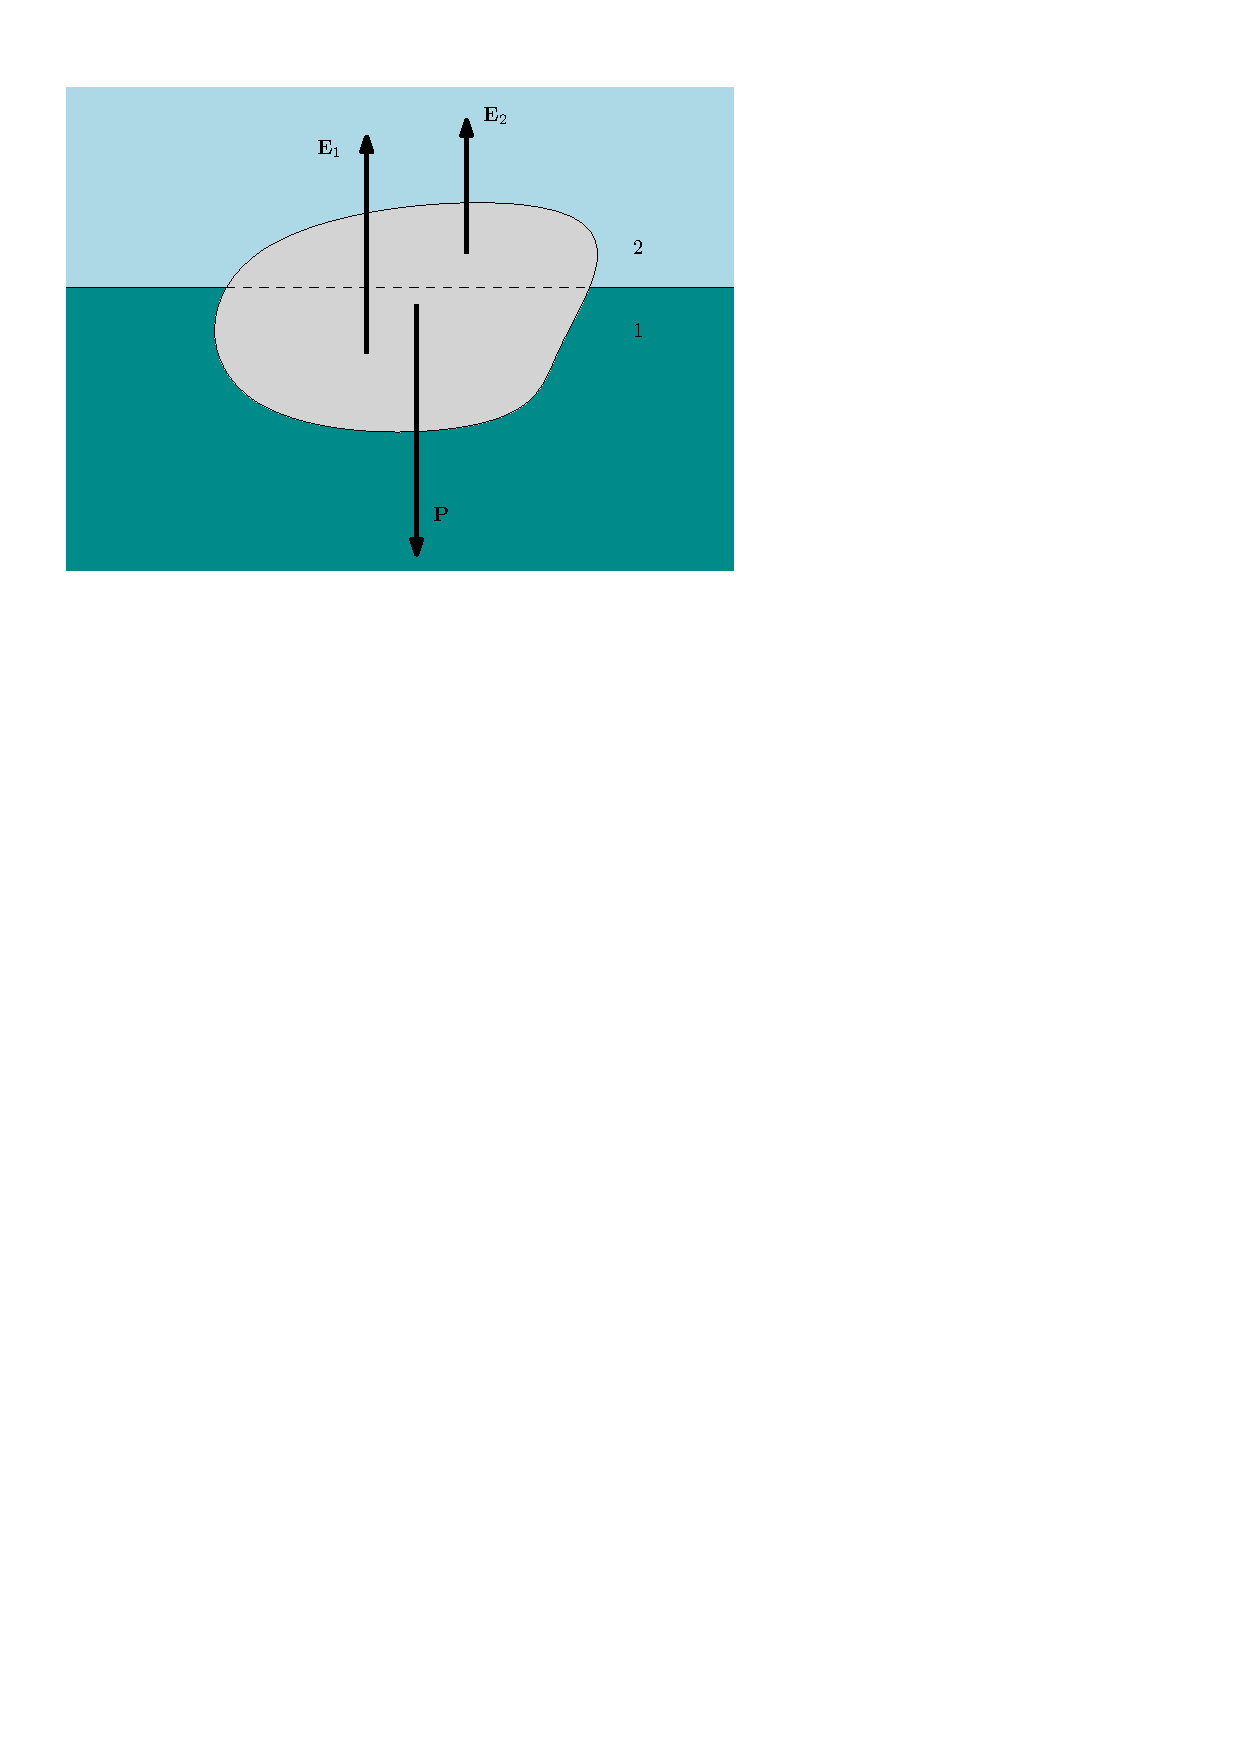
\includegraphics[width=\textwidth]{TeX_files/chapter02-Hidrostatica/arquimedes}
	\end{center}
\end{minipage}
\begin{minipage}{0.5\textwidth}
	Las lineas de acci\'on de las fuerzas de empuje y el peso no
	tienen porqu\'e coincidir, y, en este caso, se producen pares de fuerzas.
	\begin{description}
		\item[\textcolor{blue}{carena}] volumen del fluido desalojado
		\item[\textcolor{blue}{centro
			de carena} o \textcolor{blue}{centro de empuje}] centro de gravedad del fluido desalojado
	\end{description}
\end{minipage}


	El principio de Arquímedes no es, en realidad, un principio. Se puede deducir en cualquier caso simplemente calculando la integral de la presión sobre la superficie que limita el cuerpo.
	
	También se puede obervar que es la resta del peso de la columna de fluido sobre la superficie superior y sobre la superficie inferior.
	
\begin{center}
	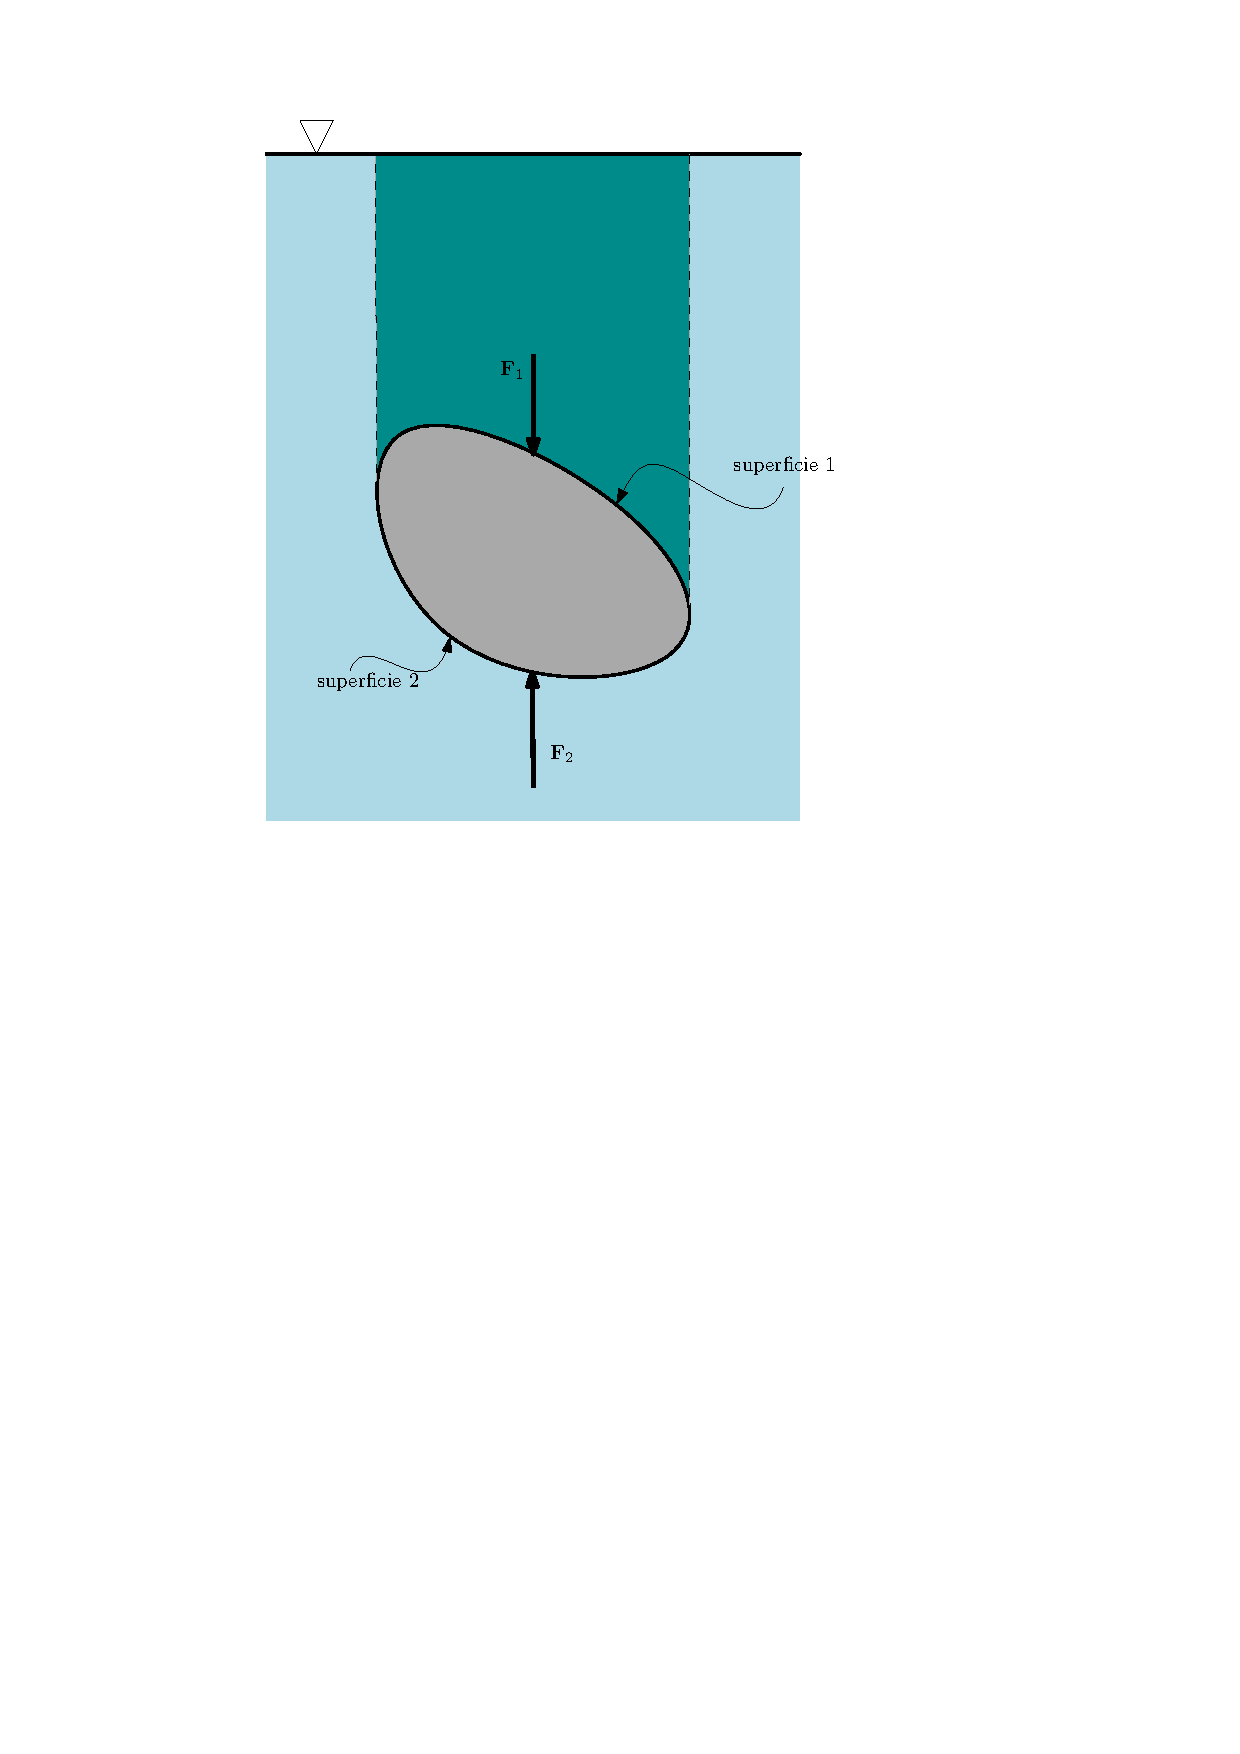
\includegraphics[width=0.5\columnwidth]{TeX_files/chapter02-Hidrostatica/arquimedes2}
\end{center}
\section{Segunda ley de Arquímedes}


	La segunda ley de Arqu\'imedes dice que \emph{un cuerpo que flota desaloja su propio peso de fluido}. 
	
	Se puede comprender observando que en la figura, el recipiente con solo fluido y el que tiene fluido y cuerpo flotando, \textbf{deben pesar lo mismo}. Pregunta: ?`C\'omo sabemos que pesan lo mismo?


	\begin{center}
		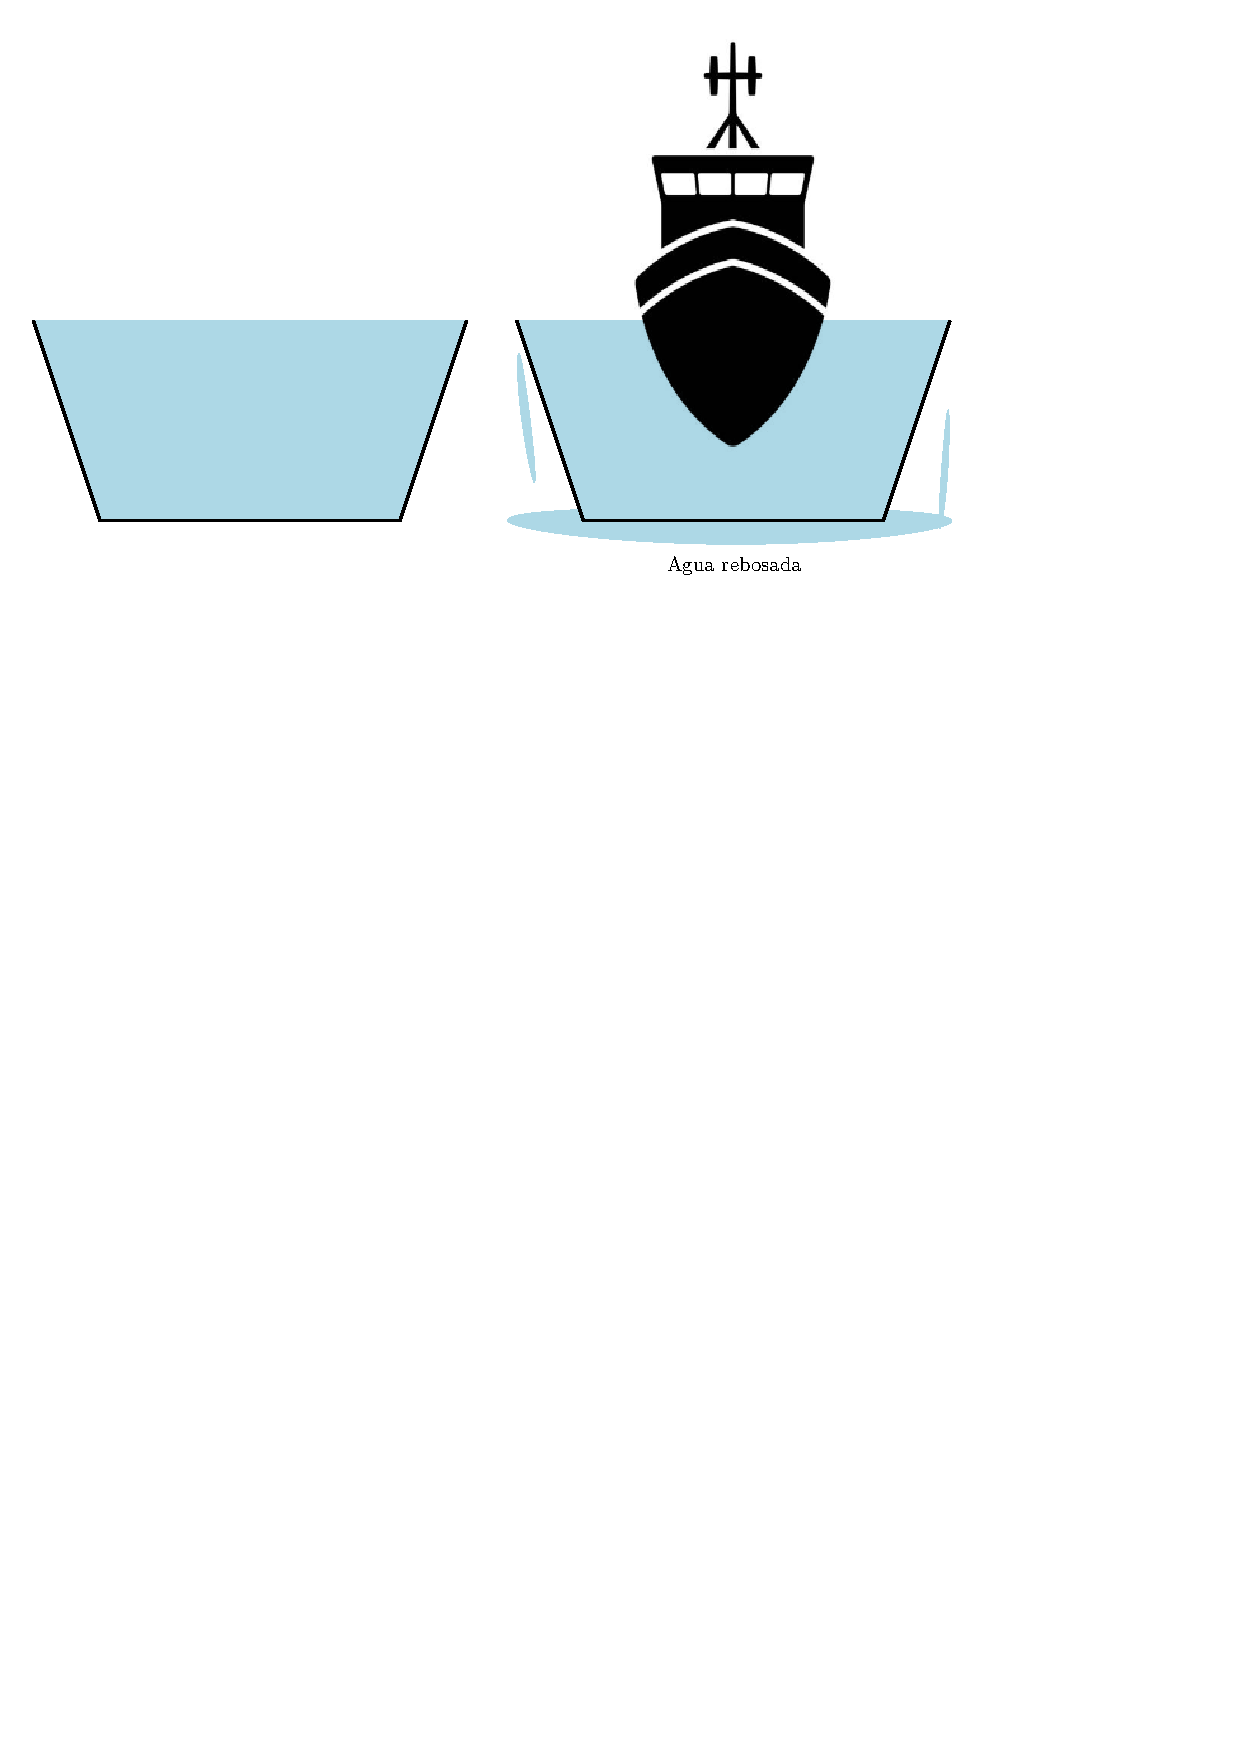
\includegraphics[width=0.75\columnwidth]{TeX_files/chapter02-Hidrostatica/arquimedes1}
	\end{center}


\section{Estabilidad}

Para un cuerpo sumergido, el centro de gravedad puede ser diferente del centro de empuje, y esto produce un momento que puede ser restaurador (equilibrio estable) o de vuelco (equilibrio inestable)

\begin{center}
	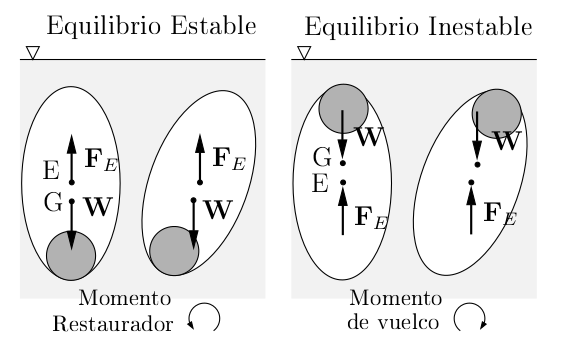
\includegraphics[width=0.7\linewidth]{TeX_files/chapter02-Hidrostatica/estabilidad1}
\end{center}

%\begin{center}
%	\includegraphics[width=0.7\columnwidth]{estab1.png}
%	% estab1.png: 996x491 pixel, 72dpi, 35.14x17.32 cm, bb=
%\end{center}


Para un cuerpo flotante, es m\'as complicado, ya que la posici\'on del centro de empuje var\'ia


Equilibrio estable 
\begin{center}
	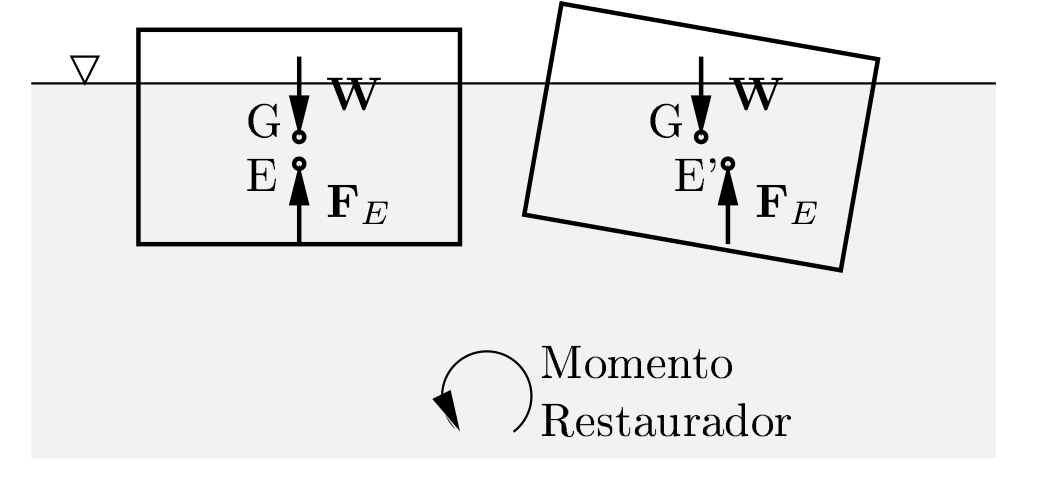
\includegraphics[width=0.7\linewidth]{TeX_files/chapter02-Hidrostatica/estabilidad2}
\end{center}



Equilibrio inestable
\begin{center}
	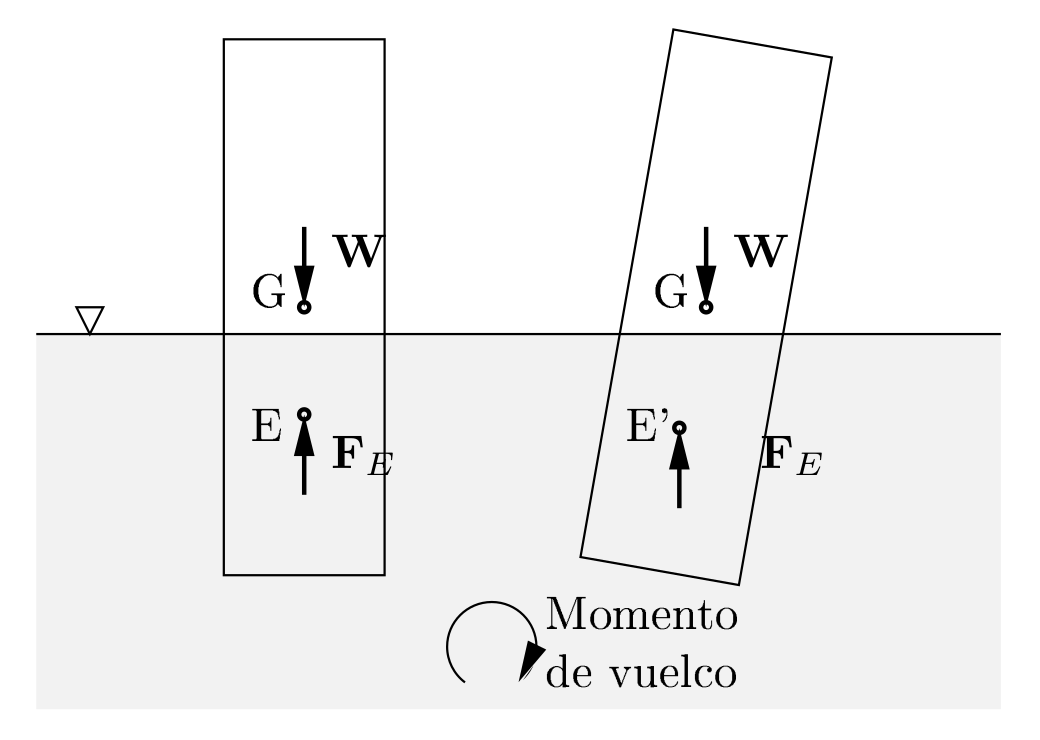
\includegraphics[width=0.7\linewidth]{TeX_files/chapter02-Hidrostatica/estabilidad3}
\end{center}


Pasos para calcular la estabilidad de un cuerpo flotante, consideremos un cuerpo sim\'etrico:

1.- Se calcula posici\'on de equilibrio inicial, mediante las fuerzas $\vec F_E$ y $\vec W$, y sus puntos de aplicaci\'on, $E$ y $G$. Como el cuerpo estan en equilibrio, estas fuerza se alinean con el eje de simetria.

2.- Se realiza una peque\~na perturbaci\'on $\Delta \theta$. El centro de empuje se desplaza a una nueva posici\'on $E'$. La vertical sobre $E'$ corta el eje de simetria en un punto $M$, denominado \textbf{metacentro}. Si el \'angulo $\Delta \theta$ es peque\~no, el metacentro no depender\'a de \'el.

3.- Se calcula la \textbf{altura metac\'entrica}, que es la distancia de $M$ a $G$. Si $M$ est\'a por encima de $G$, la altura metac\'entrica  es positiva, y la posici\'on es \emph{estable}. Si est\'a por debajo, la altura metac\'entrica es negativa, y la posici\'on es \emph{inestable}.

La altua metac\'entrica es una caracter\'istica de la secci\'on transversal del cuerpo y su distribuci\'on de masa.

\begin{center}
	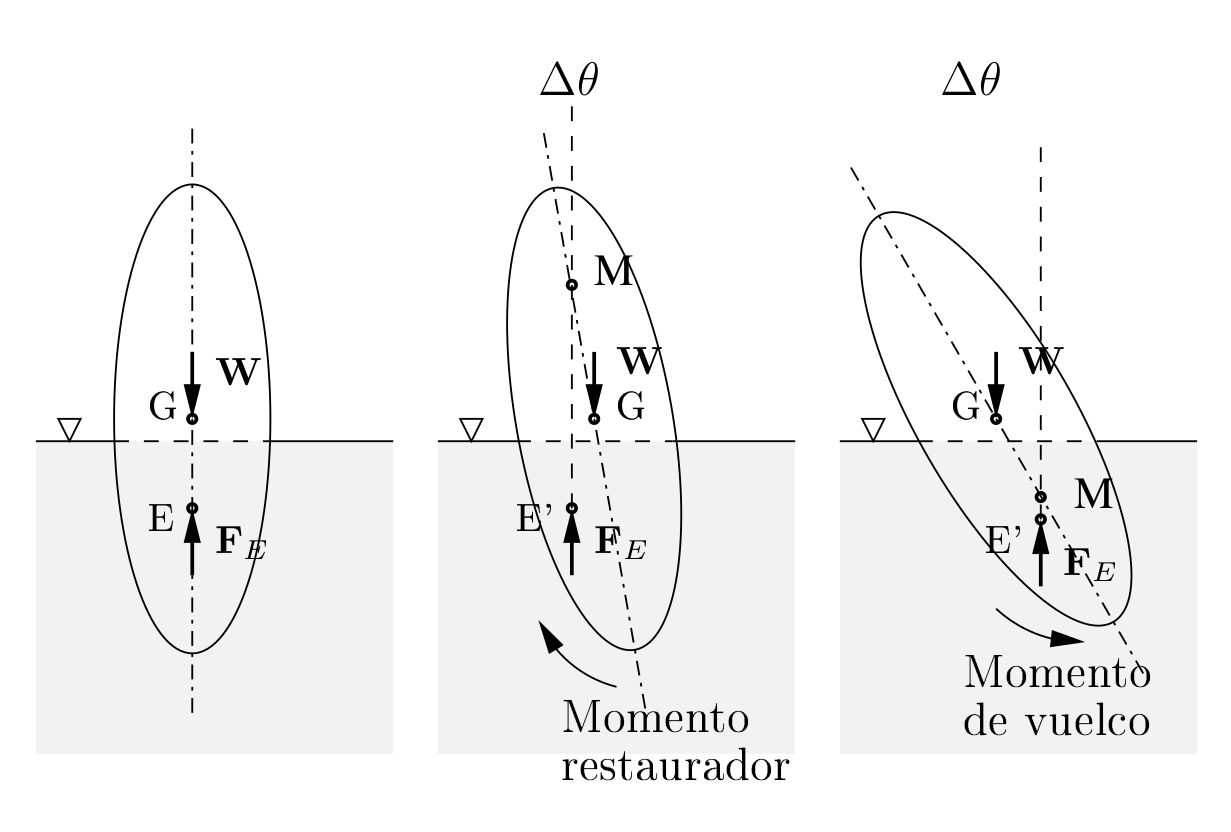
\includegraphics[width=0.7\linewidth]{TeX_files/chapter02-Hidrostatica/estabilidad4}
\end{center}

\begin{center}
	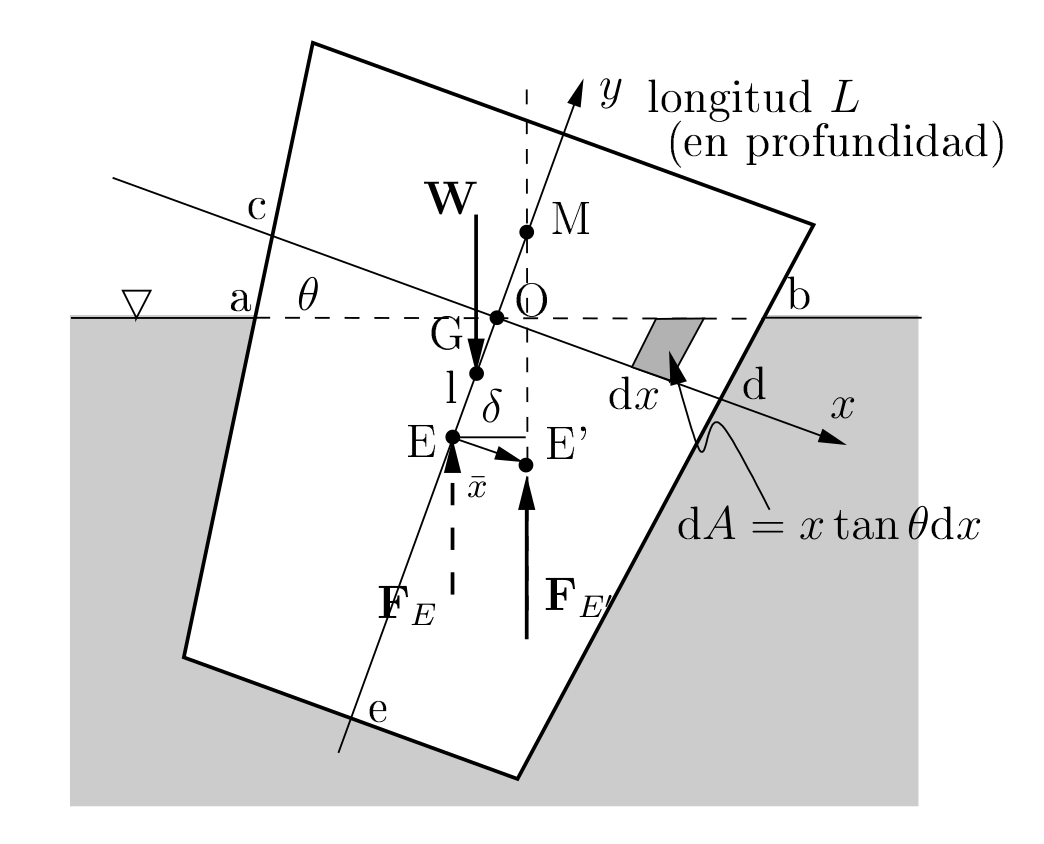
\includegraphics[width=0.7\linewidth]{TeX_files/chapter02-Hidrostatica/estabilidad5}
\end{center}




	La posici\'on del nuevo centro de empuje se calcula con la estimación del centro de masas:

\begin{align*}
	\overline{x}V_{aObdea} &= \int_{Obd}x \dif V - \int_{cOa} x \dif V
\\
	&= \int_{Obd} x L \dif A - \int_{cOa} x L \dif A 
\\
	&= \int_{Obd} x L (x\tan \theta \dif x) - \int_{cOa} x L  (-x\tan \theta \dif x)
\\
	&= \tan \theta \int x^2 2 L \dif x = \tan \theta \int x^2 \dif A 
	\\
	&= \tan \theta I_0
\end{align*}


La altura metac\'entrica es

\begin{equation}
	\overline{MG} = \overline{ME}-\overline{GE}= \frac{\overline{x}}{\tan \theta} - \overline{GE} 
= \frac{I_0}{V_{\textrm{sumergido}}} - \overline{GE} = \frac{\rho g I_0}{W} - \overline{GE}
\end{equation}

Si $\overline{MG}$ es positiva, el equilibrio es estable (para peque\~nas perturbaciones). Si 
$\overline{GE}$ es negativa, el equilibrio es estable siempre
\chapter{Cinemática de fluidos}
\section{Descripción Euleriana y Lagrangiana}
	
	Dos formas de identificación de las magnitudes (p. e., la velocidad) 
	\begin{enumerate}
		\item {\textbf{\textcolor{red}{Euleriana}}: \\
			Segun la \textcolor{blue}{posición} y el instante. 
		\begin{equation}
			\vec{u}(\vec{x},t)
		\end{equation}
		} 
		\item {\textbf{\textcolor{red}{Lagrangiana}}:\\
			Según la \textcolor{blue}{partí cula} y el instante. La partí cula
			queda identificada (marcada) mediante un vector $\vec{a}$ que puede
			ser, por ejemplo, la posición que tiene la partí cula en un instante
			de referencia $t_{0}$ 
			
\begin{equation}
				\vec{u}(\vec{a},t;t_{0})
\end{equation}
			
		} 
	\end{enumerate}


\section{Lineas de corriente, trayectorias y lineas de traza}

	
	\begin{itemize}
		\item \textcolor{red}{Lineas de corriente}:\\
		Para un instante dado $t_0$, és la tangente a los vectores de velocidad. 
	\end{itemize}

\begin{center}
	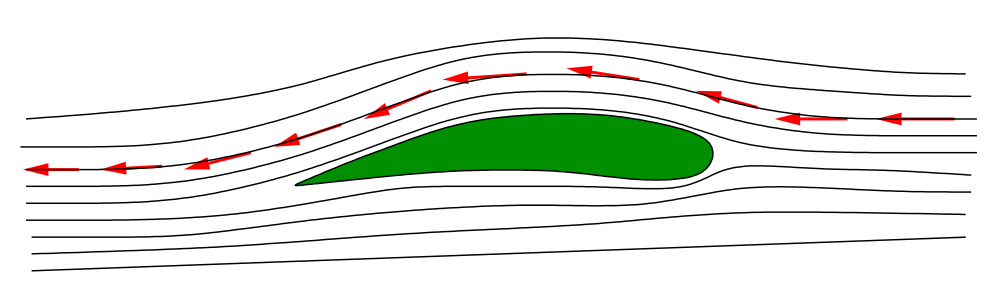
\includegraphics[width=0.7\linewidth]{TeX_files/chapter03-Cinematica/lineasCorriente}
\end{center}

		
		Són solución de la ecuación (en 2D) 
		
		\begin{equation}
			\frac{\text{d}x}{u(\vec{x},t=t_0)}=\frac{\text{d}y}{v(\vec{x},t=t_0)}
		\end{equation}
		


	
	\begin{itemize}
		\item \textcolor{red}{Trayectoria}:\\
		Para una cierta partícula de fluido, puntos que ocupa en un cierto
		intervalo de tiempo. 
		\item \textcolor{red}{Lineas de traza}:\\
		Partículas de fluido que, en un cierto instante anterior, pasaron
		por un determinado punto.
	\end{itemize}
\begin{center}
	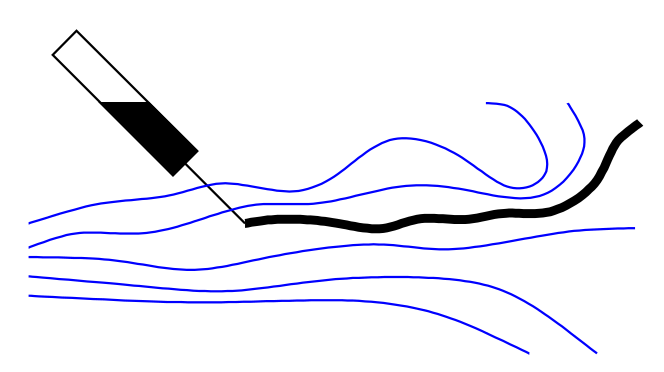
\includegraphics[width=0.5\linewidth]{TeX_files/chapter03-Cinematica/traza}
\end{center}


		
		Si el flujo es estacionario (no depende del tiempo), linea de corriente,
		trayectoria y linea de traza coinciden para un determinado punto. 
		



	
\subsection*{Actividad 1:}
		Dado el campo de velocidades bidimensional $\vec{u}=(x+t)\vec{\imath}+y\vec{\jmath}$,
		encontrad las expresiones para:
		
		a) la linea de corriente que pasa por $(1,1)$ para $t=0$
		
		b) la trayectoria de la partícula que está en $(1,1)$ para $t=0$
		
		c) la línea de traza, para $t=0$, de todas las partículas que pasaron
		por $(1,1)$


\section{Derivada sustancial}

	
	La partícula $P$, en el instante $t$ se encuentra en $\vec{x}$
	con una velocidad $\vec{u}$. La aceleración de $P$ \textbf{no} és
	$\dparc{\vec{u}}{t}$, ya que aunque $\vec{u}$ sea estacionario,
	$P$ puede estar moviéndose a un punto en que $\vec{u}$ és diferente.
	
	En un instante $t+\delta t$, $P$ estará en $\vec{x}+\delta\vec{x}=\vec{x}+\vec{u}\delta t$,
	de forma que la variación de velocidad será 
	\[
	\delta\vec{u}=\vec{u}(\vec{x}+\vec{u}\delta t,t+\delta t)-\vec{u}(\vec{x},t)
	\]
	
	Desarrollando en serie de Taylor hasta primer orden, obtenemos 
	\[
	\delta\vec{u}=\dparc{\vec{u}}{t}\delta t+(\vec{u}\cdot\vec{\nabla})\vec{u}\delta t+O(\delta t^{2}),
	\]
	de forma que la aceleración és 
	\[
	\vec{a}(\vec{x},t)=\dparc{\vec{u}}{t}+(\vec{u}\cdot\vec{\nabla})\vec{u}
	\]
	

De forma general, consideremos cualquier magnitud $f$, asociada a
una propiedad del fluido (puede ser un escalar como la temperatura,
o densidad, o la velocidad angular). 
\begin{itemize}
	\item Derivada \textcolor{red}{local}: 
	\[
	\dparc{f}{t}
	\]
	
	\item Derivada \textcolor{red}{convectiva}: 
	\[
	(\vec{u}\cdot\vec{\nabla})\vec{f}=\left(u\dparc{\phantom{f}}{x}+v\dparc{\phantom{f}}{y}+w\dparc{\phantom{f}}{z}\right)f=u_{i}\dparc{f}{x_{i}}
	\]
	
	\item Derivada \textcolor{red}{sustancial} o \textcolor{red}{total}: 
	\[
	\frac{\text{D}f}{\text{D}t}=\dparc{f}{t}+(\vec{u}\cdot\vec{\nabla})\vec{f}=\dparc{f}{t}+u_{i}\dparc{f}{x_{i}}
	\]
	
\end{itemize}

\section{Circulación, Flujo y Vorticidad}

	
	\begin{itemize}
		\item \textbf{\textcolor{red}{Circulación}}\\
		
		\[
		\Gamma=\oint_{L}\vec{u}\cdot\text{d}\vec{l}
		\]
		$L$ es cualquier contorno cerrado.
	\end{itemize}
	Si este contorno está constituido siempre por las mismas partí culas
	(es decir, es una línea material), se puede demostrar (\cite{Vir1})
	que 
	\[
	\Deriv{\Gamma}{t}=\Deriv{\phantom{t}}{t}\oint_{L}\vec{u}\cdot\text{d}\vec{l}=0
	\]
	

	
	\begin{itemize}
		\item \textbf{\textcolor{red}{Flujo}}\\
		Sea $F$ una magnitud extensiva propiedad del fluido y $f$ esta
		misma magnitud por unidad de volumen. El flujo de $f$ a través de
		la superficie $S$ es
	\end{itemize}
	\[
	\Phi=\int_{S}f\vec{u}\cdot\text{d}\vec{S}
	\]
	Si $f$ es un escalar, $f\vec{u}$ es el \textcolor{blue}{vector
		flujo} de $f$.
	
	Si $f$ es un vector $\left(\vec{f}\right)$ , $\vec{f}\vec{u}$ es
	el \textcolor{blue}{tensor flujo} de $f$.

	
{Ejemplo:}
		
		\[
		f=1\rightarrow\begin{cases}
			\vec{u} & \textrm{vector flujo volumétrico}\\
			Q=\int_{S}\vec{u}\cdot\text{d}\vec{S} & \textrm{flujo volumétrico, o caudal}
		\end{cases}
		\]
		
		\[
		f=\rho\rightarrow\begin{cases}
			\rho\vec{u} & \textrm{vector flujo másico}\\
			\dot{m}=\int_{S}\rho\vec{u}\cdot\text{d}\vec{S} & \textrm{flujo másico, o gasto}
		\end{cases}
		\]
		

\begin{itemize}
	\item \textbf{\textcolor{red}{Vorticidad}}\\
	
	\[
	\vec{\omega}=\vec{\nabla}\times\vec{u}\quad\text{En componentes:}\quad\omega_{k}=-\varepsilon_{ijk}\dparc{u_{i}}{x_{j}}
	\]
	Es el doble de la velocidad local de rotación del elemento de fluido.
	Por definición de vorticidad, se cumple que 
	\[
	\vec{\nabla}\cdot\vec{\omega}=0
	\]
	y el flujo a través de una superficie $S$ cerrada es siempre nulo
	\[
	\oint_{S}\vec{\omega}\cdot\text{d}\vec{S}=0
	\]
	\item Si la superficie es abierta, este flujo está relacionado con la circulación
	sobre la línea que limita la superficie a través del Teorema de Stokes
	\[
	\int_{S}\vec{\omega}\cdot\text{d}\vec{S}=\int_{S}\left(\vec{\nabla}\times\vec{u}\right)\cdot\text{d}\vec{S}=\oint_{L}\vec{u}\cdot\text{d}\vec{l}
	\]
	
\end{itemize}

\section{Movimiento relativo en el entorno de un punto}

	
	Sea $\vec{u}$ la velocidad del fluido en un punto $\vec{r}$. En
	un punto $\vec{r}+\delta\vec{r}$, la velocidad será $\vec{u}+\delta\vec{u}$,
	con 
	\[
	\delta\vec{u}=\vec{\nabla}\vec{u}\cdot\delta\vec{r};\ \delta u_{i}=\dparc{u_{i}}{x_{j}}\delta r_{j}
	\]
	
	El tensor \textcolor{blue}{divergencia de velocidad}, $\vec{\nabla}\vec{u}$,
	puede descomponerse como la suma de un tensor simétrico,$\left(\vec{\nabla}\vec{u}\right)^{S}$
	y un tensor antisimétrico $\left(\vec{\nabla}\vec{u}\right)^{A}$,
	con 
	\begin{eqnarray*}
		\left(\vec{\nabla}\vec{u}\right)^{S}=\frac{1}{2}\left(\vec{\nabla}\vec{u}+\left(\vec{\nabla}\vec{u}\right)^{T}\right)\\
		\left(\vec{\nabla}\vec{u}\right)^{A}=\frac{1}{2}\left(\vec{\nabla}\vec{u}-\left(\vec{\nabla}\vec{u}\right)^{T}\right)
	\end{eqnarray*}
	
	Cada uno de estos tensores contribuye a $\delta\vec{u}$ de una forma
	diferente 
	\[
	\delta\vec{u}=\delta\vec{u}^{S}+\delta\vec{u}^{A}=\left(\vec{\nabla}\vec{u}\right)^{S}\cdot\delta\vec{r}+\left(\vec{\nabla}\vec{u}\right)^{A}\cdot\delta\vec{r}
	\]
	

	
	$\delta\vec{u}^{S}=\left(\vec{\nabla}\vec{u}\right)^{S}\cdot\delta\vec{r}$
	representa un movimiento de \textcolor{blue}{deformación pura}. Siempre
	es posible escoger los ejes del sistema de referencia de forma que
	$\left(\vec{\nabla}\vec{u}\right)^{S}$ sea diagonal. Entonces los
	tres valores de la diagonal son las velocidades de estiramiento en
	la dirección de los ejes principales. Si el fluido es incompresible
	el volumen del elemento de fluido se mantiene constante y la suma
	de la diagonal, que es un invariante respecto del cambio de sistema
	de coordenadas, es nula 
	\[
	\dparc{u_{i}}{x_{i}}=0
	\]
	

	
	$\delta\vec{v}^{A}=\left(\vec{\nabla}\vec{u}\right)^{A}\cdot\delta\vec{r}$
	representa un movimiento de \textcolor{blue}{rotación pura}. 
	\[
	\delta u_{i}^{A}=\frac{1}{2}\left(\dparc{u_{i}}{x_{j}}-\dparc{u_{j}}{x_{i}}\right)\delta r_{j}=\frac{1}{2}\varepsilon_{ijk}\omega_{k}\delta r_{j}
	\]
	La velocidad angular de rotación es $\frac{1}{2}\vec{\omega}=\frac{1}{2}(\vec{\nabla}\times\vec{u})$. 


\chapter[Ecuaciones de la Dinámica]{Ecuaciones fundamentales de la Dinámica de los Fluidos}
\section{Introducción}
	
	La Mecánica de los fluidos viene determinada por \textcolor{red}{3
		leyes básicas}\footnote{Algunos autores, como \cite{Shames2003} toman en consideración también
		la Segunda Ley de la Termodinámica}
	
	\begin{itemize}
		\item \textcolor{black}{El principio de }\textcolor{red}{conservación de
			la masa}\textcolor{black}{. La masa de un sistema fluido se mantiene
			constante independientemente de su posición o forma. }
		\item \textcolor{black}{La ley de }\textcolor{red}{conservación de la cantidad
			de movimiento}\textcolor{black}{. La variación de la cantidad de movimiento
			de un sistema fluido es igual a la suma total de la fuerzas externas
			que actúan sobre él. }
		\item \textcolor{black}{La ley de }\textcolor{red}{conservación de la energía}\textcolor{black}{.
			Es, básicamente, la Primera Ley de la Termodinámica. La variación
			de la energía de un sistema fluido (energía interna + energía cinética)
			es igual al trabajo realizado por todos las fuerzas externas más el
			calor recibido por conducción y/o radiación. }
	\end{itemize}
	A estos principios hay que añadir las \textcolor{blue}{leyes constitutivas},
	como la ley de viscosidad de Newton, o la ley de los gases perfectos. 


\section{Formulación integral y diferencial}

	
	Existen dos enfoques para los problemas de Mecánica de Fluidos: 
	\begin{itemize}
		\item \textcolor{red}{Formulación diferencial}. Se consideran volumenes
		elementales de fluido y las ecuaciones que gobiernan su comportamiento.
		Para resolver los problemas con este planteamiento es necesario conocer
		las condiciones iniciales en todo el dominio y las condiciones de
		contorno en todos los límites del mismo. 
		\item \textcolor{red}{Formulación integral}. Se trabaja directamente sobre
		volumenes de fluido macroscópicos, denominados \textcolor{blue}{volúmenes
			de control}. Las ecuaciones son promediadas en el volumen de control
		y sobre su frontera, denominada \textcolor{blue}{superficie de control}. 
	\end{itemize}
	Para la mayoría de los problemas de Ingeniería ( o, por lo menos,
	para una primera aproximación) es suficiente con la formulación integral\footnote{La formulación diferencial es
		más general, y permite determinar detalles del flujo. Es posible extraer
		los resultados de la formulación integral a partir de los de la diferencial,
		pero no al contrario.}.


\subsection{Sistema y volumen de control}

	
	Un \textcolor{blue}{sistema de control} posee una cantidad definida
	de materia. Su volumen, y, por lo tanto, su densidad, así como otras
	magnitudes físicas pueden cambiar, pero no la cantidad de masa. En
	mecánica de sólidos se suele emplear el sistema de control como enfoque
	de trabajo.
	
	En Mecánica de Fluidos, es conveniente usar el enfoque de \textcolor{blue}{volúmen
		de control}, que se establece en el espacio, sin relación con una
	cierta cantidad de materia. Este volumen puede ser estático o no,
	y puede cambiar tanto de posición como de tamaño.
	
	La diferencia entre sistema y volumen de control se puede relacionar
	con la diferencia entre los puntos de vista Lagrangiano y Euleriano,
	ya que un sistema de control siempre sigue el movimiento de las partículas
	que lo componen.


\subsection{El teorema de arrastre de Reynolds}

	
	Dado que las ecuaciones de mecánica y termodinámica se refieren a
	sistemas de control, es necesario deducirlas para el caso en que las
	aplicamos sobre volúmenes de control.
	
	Consideremos un volumen de control y un sistema de control que, en
	un instante determinado $t$, coinciden en el espacio. El volumen
	de control $VC$ está estacionario, mientras que el sistema de control
	$V$ se mueve con el flujo.
	
		En el instante $t+\delta t$
				el sistema de control se encuentra en una posición ligeramente desplazada
				respecto al volumen. Incluso puede que haya cambiado su volumen, si
				el flujo es compresible
	
\begin{center}
	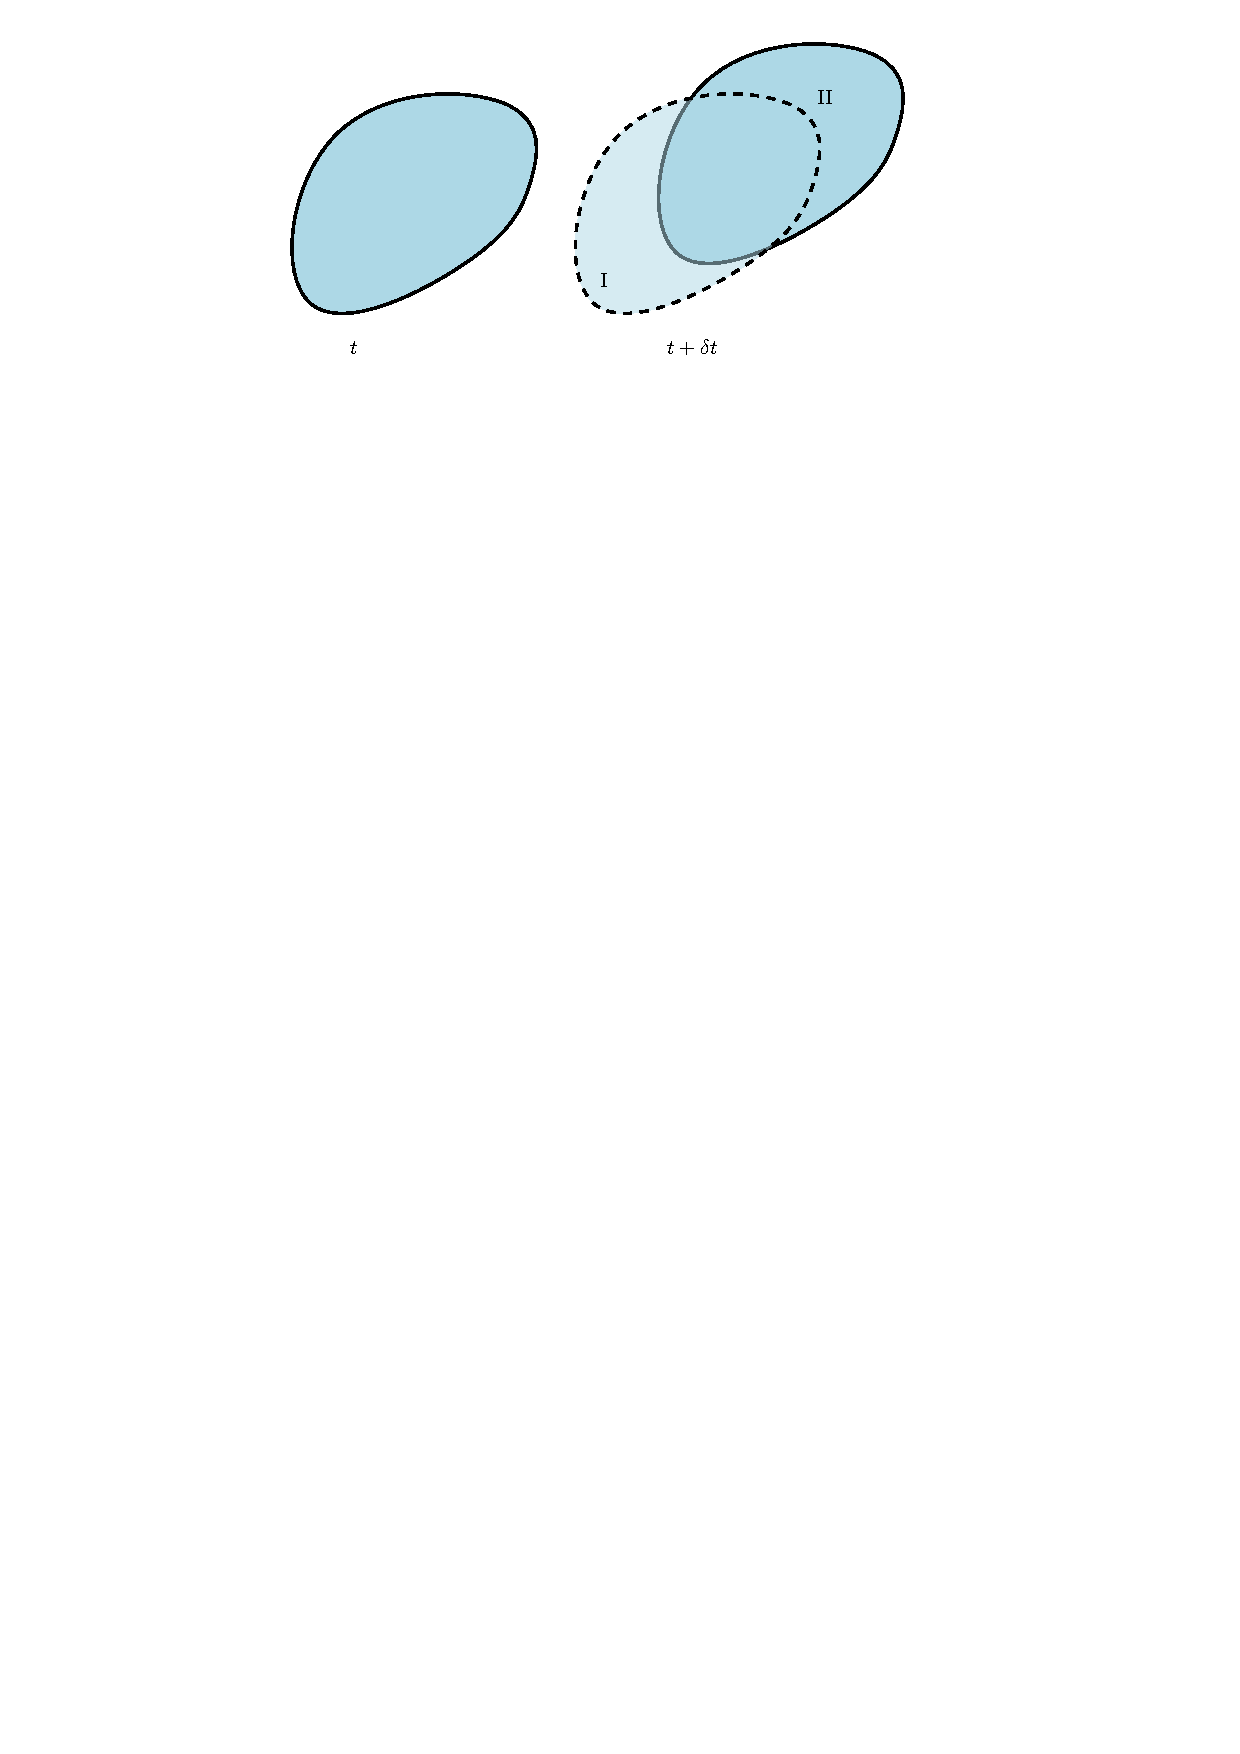
\includegraphics[width=0.7\linewidth]{TeX_files/chapter04-Dinamica/VC}
\end{center}


Consideremos una cierta magnitud extensiva $F$, y $f$ la misma por
unidad de masa, de forma que


\begin{equation}
	F=\int_{V}\rho f\,\text{d}V
\end{equation}


Consideremos la notación: \textcolor{black}{\scriptsize{}
	\begin{eqnarray*}
		F_{t} & : & \text{el valor de \ensuremath{F} para el sistema de control en el instante \ensuremath{t}}\\
		F_{t^{+}} & : & \text{el valor de \ensuremath{F} para el sistema de control en el instante \ensuremath{t+\delta t}}\\
		F'_{t} & : & \text{el valor de \ensuremath{F} para el volumen de control en el instante \ensuremath{t}}\\
		F'_{t^{+}} & : & \text{el valor de \ensuremath{F} para el volumen de control en el instante \ensuremath{t+\delta t}}\\
		F_{s} & : & \text{Cantidad de \ensuremath{F} que abandona el volumen de control en el intervalo \ensuremath{\Delta t} (a través de I)}\\
		F_{e} & : & \text{Cantidad de \ensuremath{F} que entra en el volumen de control en el intervalo \ensuremath{\Delta t} (a través de II)}
	\end{eqnarray*}
}{\scriptsize\par}

Evidentemente, 
\[
F_{t}=F'_{t}
\]


	
	Las variaciones de $F$ en el sistema de control y en el volumen de
	control son, respectivamente, 
	\begin{eqnarray*}
		\delta F & = & F_{t^{+}}-F_{t}\\
		\delta F' & = & F'_{t^{+}}-F'_{t}
	\end{eqnarray*}
	y, por otro lado, 
	\[
	F_{t^{+}}=F'_{t^{+}}+F_{s}-F_{e},
	\]
	de forma que 
	\[
	\delta F=\delta F'+F_{s}-F_{e}
	\]
	
	Dividiendo por $\delta t$ y haciendo el límite $\delta t\rightarrow0$,
	obtenemos 
	\[
	\deriv{F}{t}=\deriv{F'}{t}+\lim_{\delta t\rightarrow0}\frac{F_{s}-F_{e}}{\delta t}
	\]
	

	
	Por definición, el último término es el flujo de $F$ a través de
	la frontera de $VC$, que, como hemos definido en temas anteriores,
	
	\[
	\lim_{\delta t\rightarrow0}\frac{F_{s}-F_{e}}{\delta t}=\Phi_{F}=\oint_{SC}\rho f\vec{u}_{r}\cdot\text{d}\vec{S}
	\]
	
	\[
	\deriv{F}{t}=\deriv{F'}{t}+\oint_{SC}\rho f\vec{u}_{r}\cdot\text{d}\vec{S}
	\]
	

\begin{equation}
		\Rightarrow\boxed{\deriv{F}{t}=\deriv{\phantom{F}}{t}\int_{VC}\rho f\,\text{d}V+\oint_{SC}\rho f\vec{u}_{r}\cdot\text{d}\vec{S}}
\end{equation}
	,donde $\vec{u}_{r}$ es la velocidad del flujo relativa a la Superficie
	de Control.\\
	

	
	Otra forma de expresarlo es, usando el Teorema de Leibniz \cite[Sección 3.6]{Kundu2012}
	
\begin{equation}
		\boxed{\deriv{F}{t}=\int_{VC}\dparc{\rho f}{t}\,\text{d}V+\oint_{SC}\rho f\vec{u}\cdot\text{d}\vec{S}}
\end{equation}
	,donde $\vec{u}$ es ahora la velocidad absoluta. Si el VC no se mueve
	ni se deforma, $\vec{u}=\vec{u}_{r}$. 
	
	Se puede usar el Teorema de la Divergencia para transformar la integral
	de superficie en una integral de volumen, de forma que
	
	\[
	\deriv{F}{t}=\int_{VC}\dparc{\rho f}{t}\,\text{d}V+\int_{VC}\vec{\nabla}\cdot\left(\rho f\vec{u}\right)\text{d}V
	\]
	
	\[
	\Rightarrow\deriv{F}{t}=\int_{VC}\left[\dparc{\rho f}{t}+\vec{\nabla}\cdot\left(\rho f\vec{u}\right)\right]\text{d}V
	\]
	
\section{Ecuación integral de conservación de la masa}

	
	En este caso, $F=m$ y $f=1$. Por definición de sistema físico, $\deriv{m}{t}=0$,
	de forma que 
	\[
	\int_{VC}\dparc{\rho}{t}\,\text{d}V+\oint_{SC}\rho\vec{u}\cdot\text{d}\vec{S}=0
	\]
	
	\[
	\Rightarrow\,\boxed{\int_{VC}\dparc\rho t\,\dif V=-\oint_{SC}\rho\vec{u}\cdot\dif\vec{S}}
	\]
	
	Interpretación física: \textbf{\textcolor{red}{En un Volumen de Control,
			la variación local de la masa únicamente puede ser debida a un flujo
			de masa a través del contorno.}} 

	
	Simplicaciones de la ecuación integral de conservación de la masa
	\begin{itemize}
		\item Si el flujo es \textcolor{blue}{estacionario} en el interior del VC,
		entonces $\dparc{\rho}{t}=0$ y
		\[
		\oint_{SC}\rho\vec{u}\cdot\text{d}\vec{S}=0
		\]
		
		\item Si el flujo es \textcolor{blue}{incompresible}, entonces la densidad
		es constante en todo el VC, de forma que
		\[
		\int_{VC}\dparc\rho t\,\text{d}V=-\rho\oint_{SC}\vec{u}\cdot\text{d}\vec{S}
		\]
		
		\item Si se cumplen las dos condiciones y el flujo es \textcolor{blue}{incompresible
			y estacionario},
		\[
		\oint_{SC}\vec{u}\cdot\text{d}\vec{S}=0
		\]
	\end{itemize}


\subsection{Definición de velocidad media}

	
	Consideremos como caso simple un fluido incompresible circulando por
	una tubería. La sección de la tubería es $S$, y el flujo se puede
	considerar en todos los puntos axial, de forma que el caudal se calcula
	con 
	\[
	Q=\int_{S}u\text{d}S
	\]
	
	La \textcolor{red}{velocidad media} se define como la velocidad uniforme
	que debería tener el flujo para que el caudal fuese el mismo, $Q=\mean{u}S$.
	De aqui, 
	\[
	\mean{u}=\frac{1}{S}\int_{S}u\text{d}S
	\]
	\\
	Un documento muy interesante para estudiar la forma integral de la
	conservación de la masa, es el publicado en 2001 por el prof. Sonin,
	del MIT, disponible \href{http://web.mit.edu/2.25/www/pdf/cv.pdf}{aqui}.


\section{Ecuación diferencial de conservación de la masa}

	
	Aplicando el Teorema de la Divergencia a la forma integral, para un
	Volumen de Control estacionario, se obtiene 
	\[
	\int_{VC}\left[\dparc\rho t+\vec{\nabla}\cdot\left(\rho\vec{u}\right)\right]\text{d}V=0
	\]
	
	Como esto debe cumplirse para cualquier VC, obtenemos la forma diferencial
	de la conservación de la masa: 
	\[
	\dparc\rho t+\vec{\nabla}\cdot\left(\rho\vec{u}\right)=0
	\]
	
	En forma de componentes: 
	\[
	\dparc{\rho}{t}+\dparc{}{x_{i}}\left(\rho u_{i}\right)=0
	\]
	

\subsection{Líneas de corriente}

	
	Para un \textcolor{blue}{fluido incompresible}: 
	\[
	\vec{\nabla}\cdot\vec{u}=0
	\]
	
	\[
	\text{Flujo 2D}\quad\rightarrow\quad\dparc{u}{x}+\dparc{v}{y}=0
	\]
	
	Consideremos una función $\psi(x,y)$ que cumple 
	\[
	u=\dparc{\psi}{y}\quad;\quad v=-\dparc{\psi}{x}
	\]
	
	Entonces la ecuación de continuidad se cumple de forma exacta, ya
	que 
	\[
	\dparc{\phantom{x}}{x}\left(\dparc{\psi}{y}\right)+\dparc{\phantom{y}}{y}\left(-\dparc{\psi}{x}\right)\equiv0
	\]
	

	
	$\psi(x,y)$ es la \textcolor{red}{función de corriente}.
	
	Las líneas $\psi(x,y)=\psi_{i}=\text{cte}$ son las \textcolor{red}{líneas
		de corriente} y cumplen que 
	\[
	\text{d}\psi=0\Rightarrow\dparc{\psi}{x}\text{d}x+\dparc{\psi}{y}\text{d}y=0
	\]
	\[
	\Rightarrow-v\text{d}x+u\text{d}y=0\,\Rightarrow\,\frac{\text{d}x}{u}=\frac{\text{d}y}{v}
	\]
	
	es decir, son \emph{tangentes a $\vec{u}$} en todos los puntos

	
Interpretación física:
		
		Flujo bidimensional. Para una profundidad unidad:
		
\begin{center}
	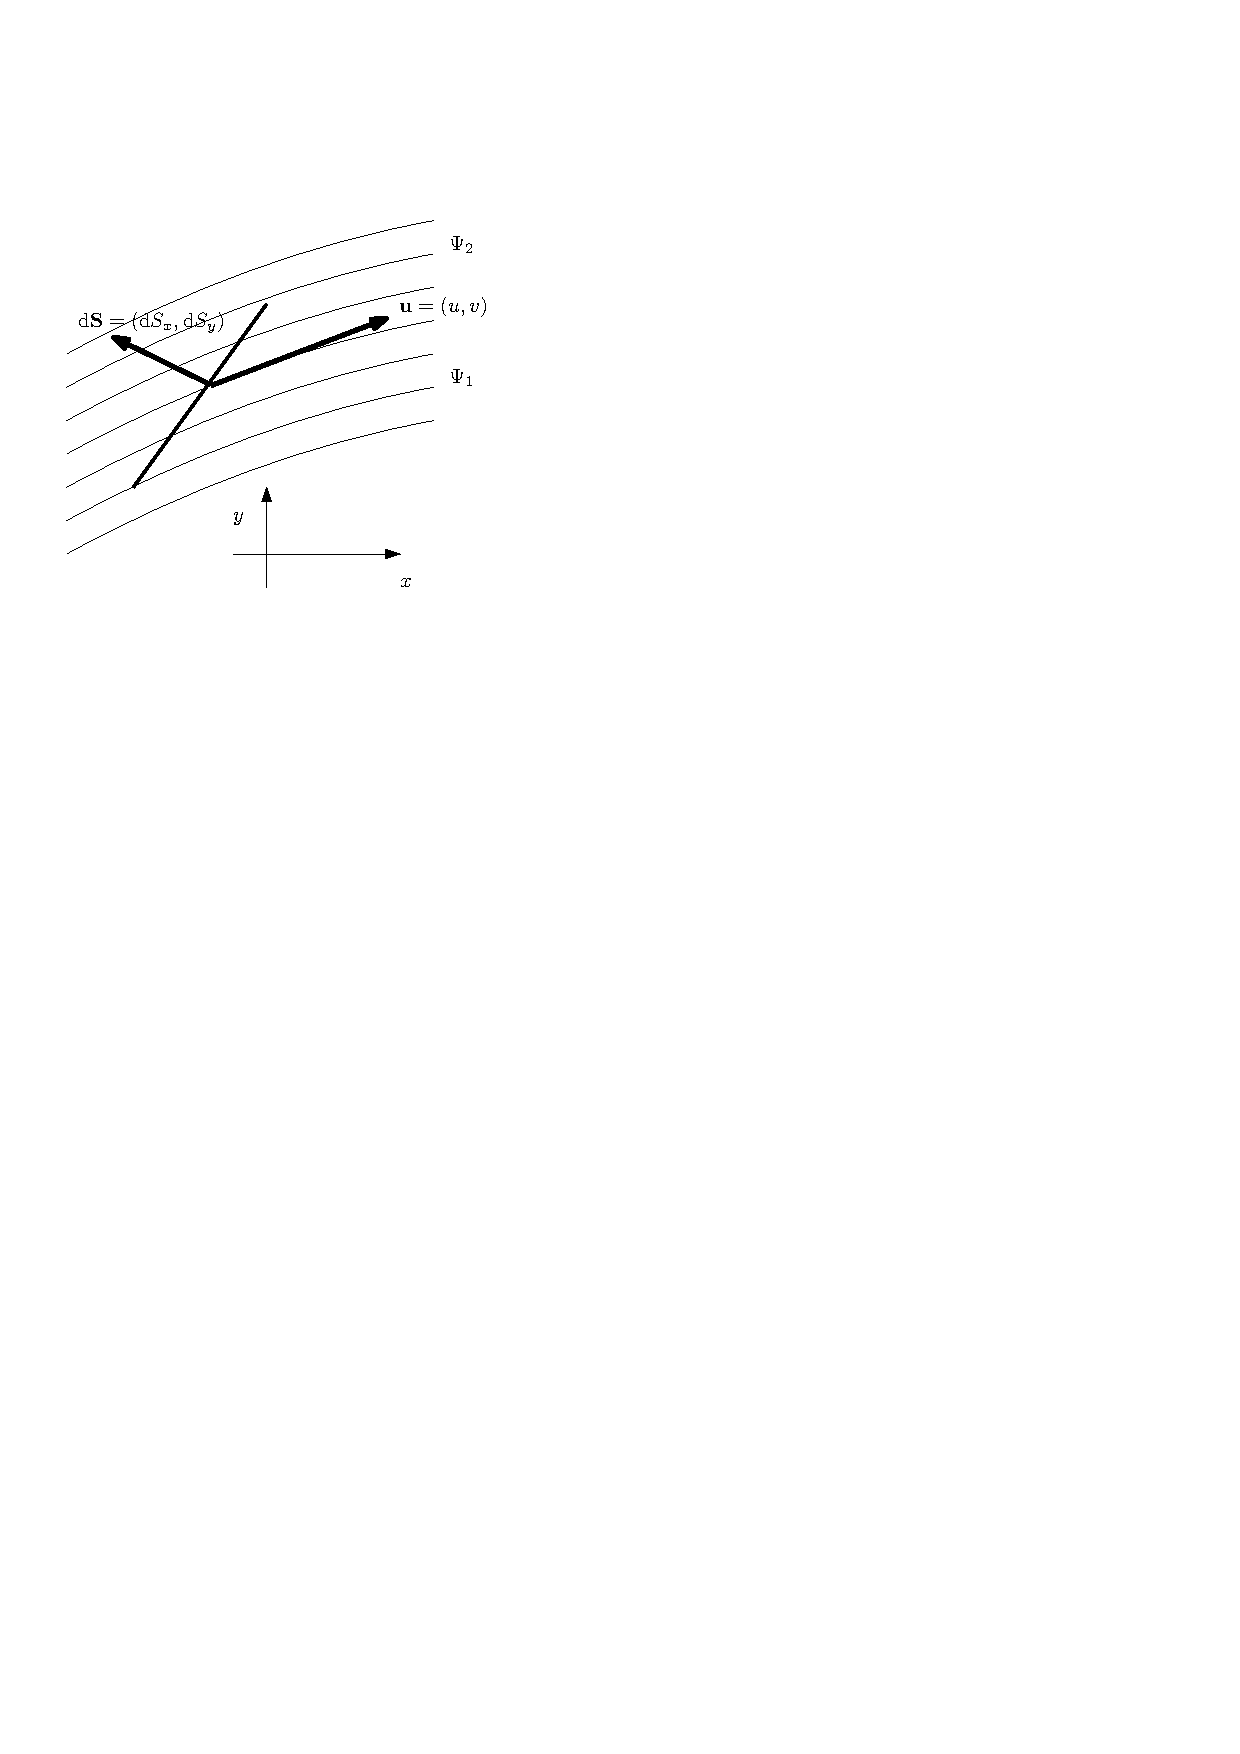
\includegraphics[width=0.4\linewidth]{TeX_files/chapter04-Dinamica/Phi1}
\end{center}

%			\input{interp_fisica_f_corr_2.pdftex_t}%
%		\end{minipage}\hfill{}%

			\begin{align*}
				dQ & =\vec{u}\cdot\text{d}\vec{S}\\
				 & =  \left(\begin{array}{cc}
					u & v\end{array}\right)\left(\begin{array}{c}
					\text{d}S_{x}\\
					\text{d}S_{y}
				\end{array}\right)\\
				& = \left(\begin{array}{cc}
					\dparc{\psi}{y} & -\dparc{\psi}{x}\end{array}\right)\left(\begin{array}{c}
					\text{d}y\\
					-\text{d}x
				\end{array}\right)(\times1)\\
				& =  \dparc{\psi}{y}\text{d}y+\dparc{\psi}{x}\text{d}x=\dif\psi\\
				\Rightarrow & \; Q=\psi_{2}-\psi_{1}
			\end{align*}


	
\subsection*{Actividad 1:}
		\[
		\vec{u}(x,y)=u(x,y)\,\vec{\imath}+v(x,y)\,\vec{\jmath}
		\]
		con $u(x,y)=a(x^{2}-y^{2})$. ?`Como tiene que ser de forma general
		$v(x,y)$ para que el flujo sea incompresible?
		
		Calcular la función de corriente y dibujar las lineas de corriente
		para el caso más simple.

\section{Ecuación integral de la conservación de la cantidad de movimiento}

	
	En este caso, $F=m\vec{u}$ y $f=\vec{u}$
	\textbf{Importante:}
		Carácter vectorial de $F$ y $f$
	
	T. de Transporte de Reynolds: 
	
	\begin{equation}
		\deriv{m\vec{u}}{t}=\deriv{\phantom{}}{t}\int_{VC}\rho\vec{u}\,\text{d}V+\oint_{SC}\rho\vec{u}\,\vec{u}_{r}\cdot\text{d}\vec{S}
	\end{equation}
	
	donde $\vec{u}_{r}$ es la velocidad relativa del fluido respecto
	de la $SC$, que no tiene por qué ser igual a $\vec{u}$, la velocidad
	relativa al Sistema de Referencia.

	
	Según la Segunda Ley de la Dinámica de Newton, 
	
\begin{equation}
		\deriv{m\vec{u}}{t}=\vec{F}_{T}
\end{equation}
	
	donde $\vec{F}$ es la suma total de \underline{todas} las fuerzas
	que actúan sobre el $VC$, tanto \textcolor{blue}{superficiales} como
	\textcolor{blue}{másicas}. Las fuerzas superficiales són producidas
	por todos los \textcolor{blue}{fluidos} y \textcolor{blue}{sólidos}
	incluidos en el $VC$.
	
	Debido al caracter vectorial de la cantidad de movimiento: 
	\begin{eqnarray}
		{F_{T}}_{x} & = & \deriv{\phantom{}}{t}\int_{VC}\rho u\,\text{d}V+\oint_{SC}\rho u\,\vec{u}_{r}\cdot\text{d}\vec{S}\\
		{F_{T}}_{y} & = & \deriv{\phantom{}}{t}\int_{VC}\rho v\,\text{d}V+\oint_{SC}\rho v\,\vec{u}_{r}\cdot\text{d}\vec{S}\\
		{F_{T}}_{z} & = & \deriv{\phantom{}}{t}\int_{VC}\rho w\,\text{d}V+\oint_{SC}\rho w\,\vec{u}_{r}\cdot\text{d}\vec{S}
	\end{eqnarray}
	


\section{Cálculo de fuerzas en un $VC$}

	
	Supongamos, por simplicidad, que el $VC$ está en reposo respecto
	del SR inercial.
	
	Las fuerzas superficiales que actúan sobre el material del VC són 
	\begin{itemize}
		\item tensiones de los sólidos que atraviesan el $VC$. 
		\item esfuerzos normales (presión) y tangenciales del fluido.\\
		Cálculo de presiones: 
		\[
		\vec{F}_{p}=-\oint_{SC}p\,\text{d}\vec{S}
		\]
		Si la presión és uniforme en toda la $SC$, $\vec{F}_{p}=0$. 
	\end{itemize}

	
	En muchas ocasiones los problemas prácticos de Ingeniería relacionados
	con la ecuación integral del conservación de la cantidad de movimiento
	són, básicamente, encontrar la fuerza que se ejerce sobre un cierto
	sólido en contacto con un fluido en movimiento.
	
	Ejemplos: 
	\begin{itemize}
		\item Fuerza sobre uniones en tuberías. 
		\item Fuerza sobre toberas, inyectores, \ldots{} 
		\item Fuerza sobre un vehículo aéreo o espacial. 
		\item Fuerza de un chorro sobre un obstáculo. 
		\item Fuerza sobre un vertedero. 
		\item \ldots{} 
	\end{itemize}
	La fuerza que se quiere calcular es siempre uno de los términos de
	$\vec{F}_{T}$. La raiz del problema estriba en aislar éste término
	en la relación de conservación de la cantidad de movimiento.

	
	\subsection*{Ejemplo (extraido de \cite{White2008}):}
		
\begin{center}
	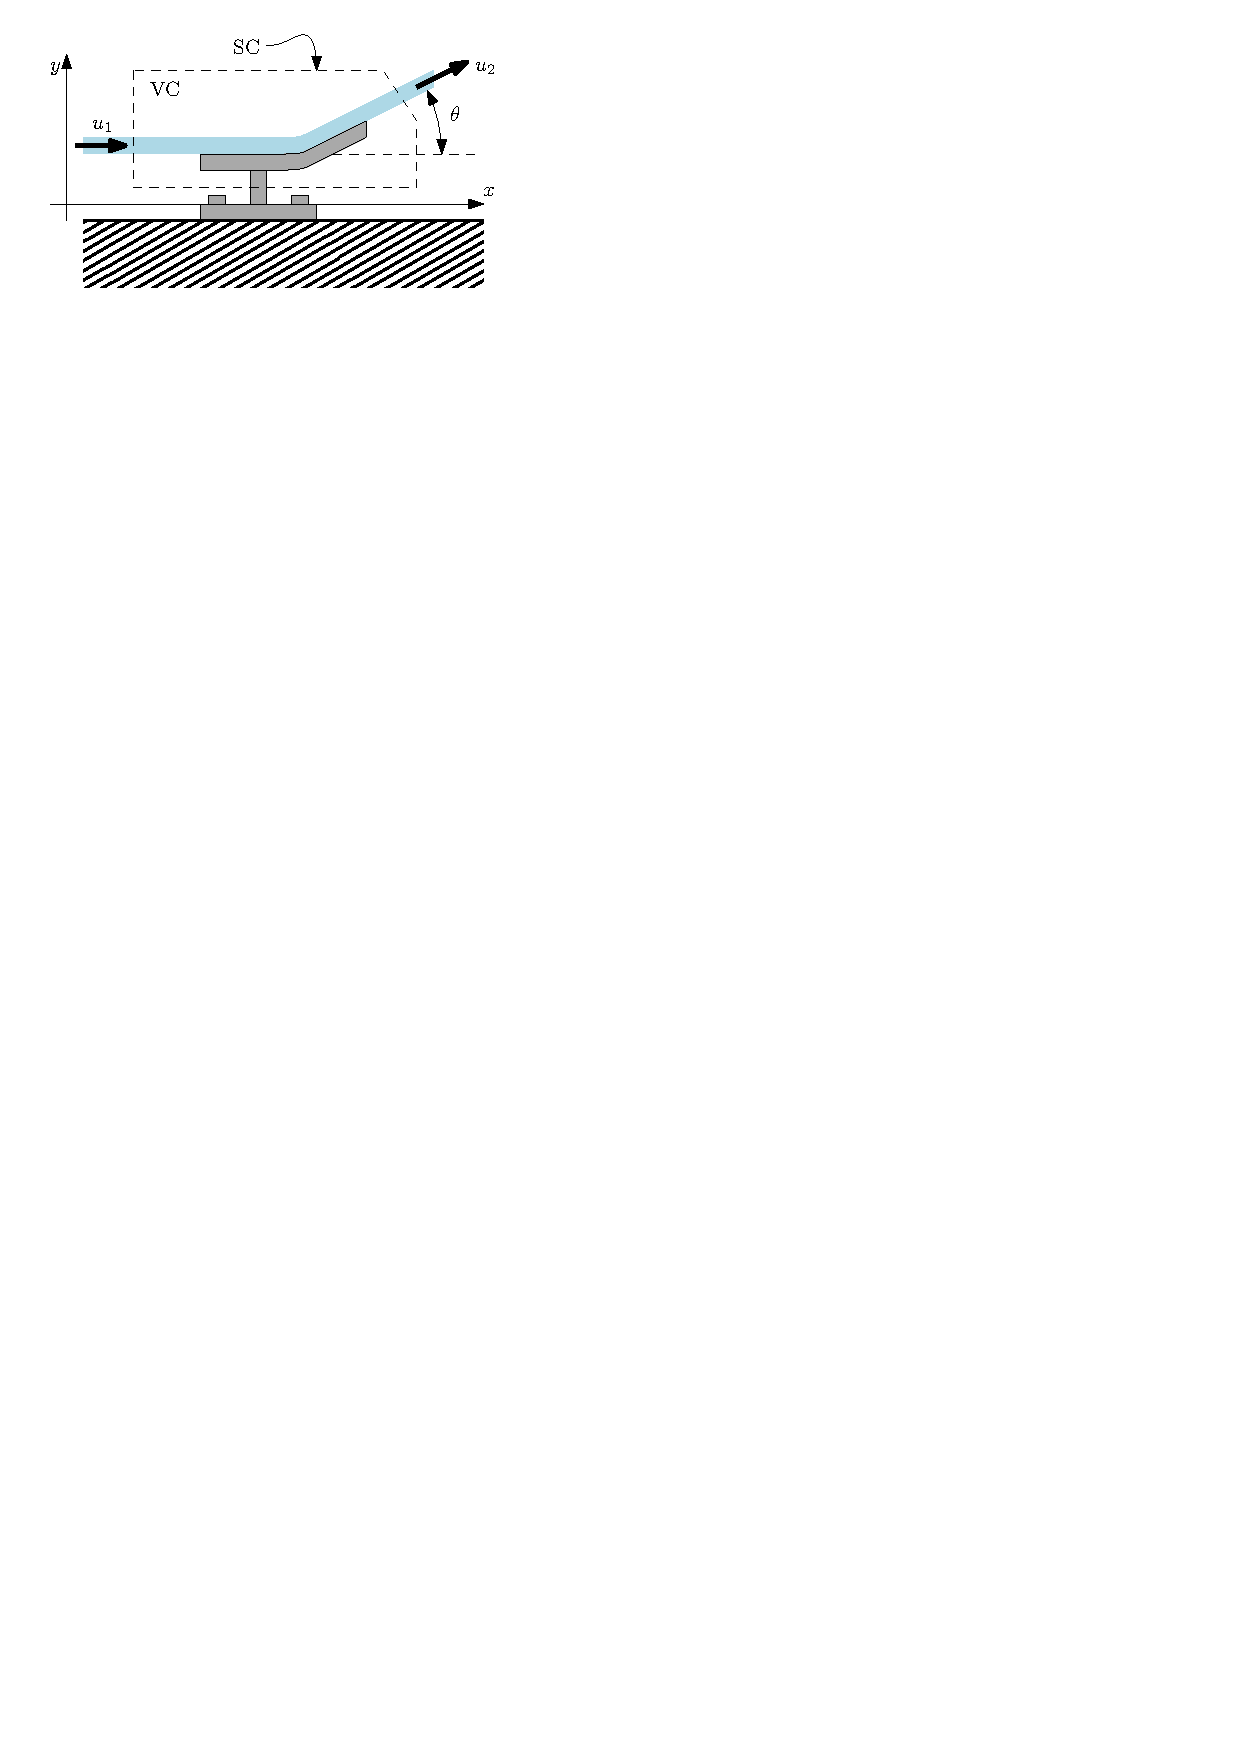
\includegraphics[width=0.5\linewidth]{TeX_files/chapter04-Dinamica/ejemploCM}
\end{center}

		
		Como hipótesis, suponemos que la sección del chorro es idéntica a
		la entrada y a la salida, de forma que, por la conservación de la
		masa, $\|\vec{u}_{1}\|=\|\vec{u}_{2}\|$.
		
		Queremos calcular la fuerza $\vec{F}$ que ejerce el chorro sobre
		el soporte.
		
		En realidad, lo que calcularemos será la fuerza $\vec{F}'$ que ejerce
		el soporte sobre el chorro. 
		
		Según la 3a. Ley de la Dinámica de Newton, $\vec{F}=-\vec{F}'$.

	

		\[
		\vec{F}'+\vec{F}_{m}+\vec{F}_{s}=\deriv{\phantom{}}{t}\int_{VC}\rho\vec{u}\,\text{d}V+\oint_{SC}\rho\vec{u}\,\vec{u}_{r}\cdot\text{d}\vec{S}
		\]
		$\vec{F}_{m}$: \emph{Fuerza de la gravedad.} Dado que no tenemos
		información sobre el volumen del chorro en el interior del VC, adoptamos
		la hipótesis de que $\|\vec{F}_{m}\|$ será muy pequeño en comparación
		con el resto de términos y, por lo tanto, lo despreciamos. A posteriori,
		debería comprobarse la validez de esta hipótesis.
		
		$\vec{F}_{s}$: \emph{Fuerza superficiales}, que engloban la presión
		y los esfuerzos tangenciales (fricción). Dado que la presión es uniforme,
		se anula. En cuanto a las fuerzas debidas a la fricción no hay ningun
		argumento para calcularlas, de forma que adoptamos la hipótesis de
		que són menospreciables.


		En cuanto al segundo miembro, el chorro es estacionario en el interior
		del VC, de forma que $\deriv{\phantom{}}{t}\int_{VC}\rho\vec{u}\,\text{d}V=0$
		
		La conservación de la cantidad de movimiento queda como 
		\[
		\vec{F}'=\oint_{SC}\rho\vec{u}\,\vec{u}\cdot\text{d}\vec{S}
		\]
		
		La velocidad sólo está definida en las secciones $S_{1}$ y $S_{2}$
		de $SC$, de forma que 
		\[
		\vec{F}'=\int_{S_{1}}\rho\vec{u}\,\vec{u}\cdot\text{d}\vec{S}+\int_{S_{2}}\rho\vec{u}\,\vec{u}\cdot\text{d}\vec{S}
		\]
		En componentes, según el SR de la figura, 
		\begin{eqnarray*}
			F'_{x} & = & \int_{S_{1}}\rho u\,\vec{u}\cdot\text{d}\vec{S}+\int_{S_{2}}\rho u\,\vec{u}\cdot\text{d}\vec{S}\\
			F'_{y} & = & \int_{S_{1}}\rho v\,\vec{u}\cdot\text{d}\vec{S}+\int_{S_{2}}\rho v\,\vec{u}\cdot\text{d}\vec{S}
		\end{eqnarray*}

	
		Es fácil ver que 
		\[
		\begin{array}{cc}
			\begin{cases}
				u=u & \text{en}\;S\\
				v=0 & \text{en}\;S_{1}
			\end{cases} & \begin{cases}
				u=u\cos\theta & \text{en}\;S_{2}\\
				v=u\sin\theta & \text{en}\;S_{2}
		\end{cases}\end{array}
		\]
		De forma que 
		\[
		\left\{ \begin{array}{ll}
			F'_{x} & =\int_{S_{1}}\rho u\vec{u}\cdot\text{d}\vec{S}+\int_{S_{2}}\rho u\cos\theta\vec{u}\cdot\text{d}\vec{S}\\
			& =\rho v\int_{S_{1}}\vec{u}\cdot\text{d}\vec{S}+\rho u\cos\theta\int_{S_{2}}\vec{u}\cdot\text{d}\vec{S}\\
			F'_{y} & =\int_{S_{2}}\rho u\sin\theta\vec{u}\cdot\text{d}\vec{S}=\rho u\sin\theta\int_{S_{2}}\vec{u}\cdot\text{d}\vec{S}
		\end{array}\right.
		\]
		
		\[
		\Rightarrow\left\{ \begin{array}{l}
			F'_{x}=\rho u(-Q)+\rho u\cos\theta Q=\rho uQ(cos\theta-1)\\
			F'_{y}=\rho u\sin\theta Q
		\end{array}\right.
		\]
		
		\[
		\Rightarrow\fbox{\ensuremath{\left\{  \begin{array}{l}
					F_{x}=\rho Su^{2}(1-\cos\theta)\\
					F_{y}=-\rho Su^{2}\sin\theta
				\end{array}\right.}}
		\]

	
	\subsection*{Actividad 1:}
		Una manguera antiincendios, de 10 cm de diámetro, da 100 l/s de
		agua con una presión de 1600 kPa. Al final de la manguera hay un inyector
		que reduce el diámetro a 2,5 cm. Estima suponiendo que ésta és la
		presión al llegar el agua al inyector, la fuerza que ejerce el agua
		sobre el mismo.


\subsection{Sistema de Referencia No Inercial}
	
	El SR está ahora acelerado. La conservación de la cantidad de movimiento
	es 
	\[
	\vec{F}_{T}-\int_{VC}\rho\vec{a}'\text{d}V=\int_{VC}\dparc{\rho\vec{u}}{t}\,\text{d}V+\oint_{SC}\rho\vec{u}\,\vec{u}\cdot\text{d}\vec{S}
	\]
	donde 
	\[
	\vec{a}'=\underbrace{\frac{\text{d}^{2}\vec{R}}{\text{d}t^{2}}}_{\text{ac. lineal del SR}}+\underbrace{\deriv{\vec{\Omega}}{t}\times\vec{r}}_{\text{ac. angular del SR}}+\underbrace{2\left(\vec{\Omega}\times\vec{u}\right)}_{\text{ac. de Coriolis}}+\underbrace{\vec{\Omega}\times\left(\vec{\Omega}\times\vec{r}\right)}_{\text{ac. centr\'\i fuga}}
	\]
	


\subsection{Factor de corrección de flujo de cantidad de movimiento}

	
	Flujo de cantidad de movimiento: 
	\[
	\Phi=\int_{S}\rho\vec{u}\left(\vec{u}\cdot\text{d}\vec{S}\right)
	\]
	
	Supongamos que $\vec{u}\parallel\text{d}\vec{S}$ y $\vec{u}=u\vec{\imath}$
	en todo $S$ (p. e., en una tubería), de forma que $\Phi=\int_{S}\rho u^{2}\text{d}S$
	
	A veces es conveniente relacionarlo con la velocidad media, $\Phi=\beta\rho\overline{u}^{2}S$,
	donde $\beta>1$ es un factor de conversión, que se calcula mediante
	\[
	\beta=\frac{1}{S}\int\left(\frac{u}{\overline{u}}\right)^{2}\text{d}S
	\]
	si el fluido es incompresible.
	\subsection*{Actividad 2:}
		
		Calcular el valor de $\beta$ para un perfil parabólico de velocidad. 

\section{Ecuación diferencial de la conservación de la cantidad de movimiento}

	
	La ecuación integral es, aplicando el TRR: 
	
	\begin{equation}
		\int_{VC}\dparc{\phantom{t}}{t}\left(\rho\vec{u}\right)\text{d}V+\oint_{SC}\rho\vec{u}\left(\vec{u}\cdot\text{d}\vec{S}\right)=\vec{F}_{T}
	\end{equation}
	
	
	Aplicando el Teorema de la Divergencia a la integral sobre la Superficie
	de Control (ver, p.e., \cite{Liggett1994}, pag. 6), 
	
	\begin{equation}
		\oint_{SC}\rho\vec{u}\left(\vec{u}\cdot\text{d}\vec{S}\right)=\int_{VC}\vec{\nabla}\cdot\left(\vec{u}\rho\vec{u}\right)\text{d}V
	\end{equation}
	
	obtenemos 
	
	\begin{equation}
		\int_{VC}\left[\dparc{\phantom{t}}{t}\left(\rho\vec{u}\right)+\vec{\nabla}\cdot\left(\vec{u}\rho\vec{u}\right)\right]\text{d}V=\vec{F}_{T}
	\end{equation}
	
	
	
	Por tanto, la fuerza sobre un volumen elemental de fluido es 
	\begin{eqnarray}
		\vec{f}_{T} & = & \dparc{\phantom{t}}{t}\left(\rho\vec{u}\right)+\vec{\nabla}\cdot\left(\vec{u}\rho\vec{u}\right)\\
		& = & \dparc{\phantom{t}}{t}\left(\rho\vec{u}\right)+\dparc{\phantom{x}}{x}\left(\rho u\vec{u}\right)+\dparc{\phantom{y}}{y}\left(\rho v\vec{u}\right)+\dparc{\phantom{z}}{z}\left(\rho w\vec{u}\right)
	\end{eqnarray}
	
	En forma de componentes: 
	\begin{eqnarray}
		{f_{T}}_{x} & = & \dparc{\phantom{t}}{t}\left(\rho u\right)+\dparc{\phantom{x}}{x}\left(\rho u^{2}\right)+\dparc{\phantom{y}}{y}\left(\rho vu\right)+\dparc{\phantom{z}}{z}\left(\rho wu\right)\\
		{f_{T}}_{y} & = & \dparc{\phantom{t}}{t}\left(\rho v\right)+\dparc{\phantom{x}}{x}\left(\rho uv\right)+\dparc{\phantom{y}}{y}\left(\rho v^{2}\right)+\dparc{\phantom{z}}{z}\left(\rho wv\right)\\
		{f_{T}}_{z} & = & \dparc{\phantom{t}}{t}\left(\rho w\right)+\dparc{\phantom{x}}{x}\left(\rho uw\right)+\dparc{\phantom{y}}{y}\left(\rho vw\right)+\dparc{\phantom{z}}{z}\left(\rho w^{2}\right)
	\end{eqnarray}
	

	
	Podemos simplificar un poco usando 
	\begin{eqnarray}
		\dparc{\phantom{t}}{t}\left(\rho\vec{u}\right) & = & \vec{u}\,\dparc{\rho}{t}+\rho\,\dparc{\vec{u}}{t}\\
		\dparc{\phantom{x}}{x}\left(\rho u\vec{u}\right) & = & \vec{u}\,\dparc{\rho u}{x}+\rho u\,\dparc{\vec{u}}{x}\\
		\dparc{\phantom{y}}{y}\left(\rho v\vec{u}\right) & = & \vec{u}\,\dparc{\rho v}{y}+\rho v\,\dparc{\vec{u}}{y}\\
		\dparc{\phantom{z}}{z}\left(\rho w\vec{u}\right) & = & \vec{u}\,\dparc{\rho w}{x}+\rho w\,\dparc{\vec{u}}{z}
	\end{eqnarray}
	
	\begin{eqnarray}
		\Rightarrow\vec{f}_{T} & = & \vec{u}\,\dparc{\rho}{t}+\rho\,\dparc{\vec{u}}{t}+\vec{u}\left(\vec{\nabla}\cdot\rho\vec{u}\right)+\rho\left(\vec{u}\cdot\nabla\right)\vec{u}\\
		& = & \vec{u}\cdot\underbrace{\left[\dparc{\rho}{t}+\vec{\nabla}\cdot\rho\vec{u}\right]}_{=0\;\text{por continuidad}}+\rho\,\dparc{\vec{u}}{t}+\rho\left(\vec{u}\cdot\vec{\nabla}\right)\vec{u}
	\end{eqnarray}
	

	
	La \textcolor{red}{ecuación diferencial de conservación de la cantidad
		de movimiento} queda como 
	
	\begin{equation}
		\boxed{\vec{f}_{T}=\rho\,\dparc{\vec{u}}{t}+\rho\left(\vec{u}\cdot\vec{\nabla}\right)\vec{u}}
	\end{equation}
	
	
	Para simplificar, supongamos que 
	\[
	\vec{f}_{T}=\text{gravedad}+\text{fricción fluido-fluido}
	\]
	
	\[
	\vec{f}_{T}=\rho\vec{g}+\vec{\nabla}\cdot\vec{\vec{\tau}}
	\]
	de forma que 
	
	\begin{equation}
		\rho\,\dparc{\vec{u}}{t}+\rho\left(\vec{u}\cdot\vec{\nabla}\right)\vec{u}=\rho\vec{g}+\vec{\nabla}\cdot\vec{\vec{\tau}}
	\end{equation}
	
	
	En forma de componentes: 
	
	\begin{equation}
		\rho\left(\dparc{u_{i}}{t}+u_{j}\dparc{u_{i}}{x_{j}}\right)=\rho g_{i}+\dparc{\tau_{ij}}{x_{j}}
	\end{equation}
	
	

\section{El tensor de tensiones para fluidos newtonianos. La ecuación de Navier-Stokes}

	
	El mayor problema de la ecuación anterior es el cálculo de $\vec{\vec{\tau}}$.
	Éste tensor agrupa tanto los esfuerzos normales como los tangenciales.
	
	Los esfuerzos normales no són la presión, ya que ésta no está definida
	de forma estricta para fluidos en movimiento(ver \cite{Batchelor1997},
	capítulo 3), pero se puede definir una presión análoga a la usada
	en fluidostática de la forma $p=-\frac{1}{3}\tau_{ii}$
	
	De esta forma, el tensor de tensiones es 
	\[
	\tens=\underbrace{-p\mathbb{I}}_{\text{parte isótropa}}+\underbrace{\tens'}_{\begin{footnotesize}\begin{array}{c}
				\text{parte anisótropa (con traza nula)}\end{array}\end{footnotesize}}
	\]
	
	\[
	=\left(\begin{array}{ccc}
		-p & 0 & 0\\
		0 & -p & 0\\
		0 & 0 & -p
	\end{array}\right)+\left(\begin{array}{ccc}
		\tau_{xx}+p & \tau_{xy} & \tau_{xz}\\
		\tau_{yx} & \tau_{yy}+p & \tau_{yz}\\
		\tau_{zx} & \tau_{zy} & \tau_{zz}+p
	\end{array}\right)
	\]
	
	
	Se puede demostrar(ver, p.e., \cite{Batchelor1997} o \cite{CrespoMartinez2006})
	que, para \textcolor{blue}{fluidos newtonianos}, $\tens'$ está relacionado
	con la parte simétrica de la divergencia de la velocidad (ver el segundo
	tema de cinemática) mediante 
	
\begin{equation}
		\tens'=2\mu\left[\left(\vec{\nabla}\vec{u}\right)^{S}-\frac{1}{3}\left(\vec{\nabla}\cdot\vec{u}\right)\mathbb{I}\right]
\end{equation}
	
	donde $\mu$ es la viscosidad dinámica.
	
	Substituyendo en la ecuación diferencial de la conservación de la
	cantidad de movimiento, 
	
	\begin{equation}
		\rho\,\dparc{\vec{u}}{t}+\rho\left(\vec{u}\cdot\vec{\nabla}\right)\vec{u}=\rho\vec{g}-\vec{\nabla}p+\vec{\nabla}\cdot\left\{ 2\mu\left[\left(\vec{\nabla}\vec{u}\right)^{S}-\frac{1}{3}\left(\vec{\nabla}\cdot\vec{u}\right)\mathbb{I}\right]\right\}
	\end{equation}
	
	,que es la \textcolor{red}{ecuación de Navier-Stokes}.

	
	En la mayoría de los casos, se puede considerar que \textcolor{blue}{$\mu$
		es uniforme}, de forma que, tras algunas operaciones tensoriales,
	
	\begin{equation}
		\rho\,\dparc{\vec{u}}{t}+\rho\left(\vec{u}\cdot\vec{\nabla}\right)\vec{u}=\rho\vec{g}-\vec{\nabla}p+\mu\left[\triangle\vec{u}+\frac{1}{3}\vec{\nabla}\left(\vec{\nabla}\cdot\vec{u}\right)\right]
	\end{equation}
	
	con 
	
	\begin{equation}
		\laplace\equiv{\vec{\nabla}}^{2}=\dparcsec{\phantom{x}}{x}+\dparcsec{\phantom{y}}{y}+\dparcsec{\phantom{z}}{z}
	\end{equation}
	
	
	Si el \textcolor{blue}{flujo es incompresible}, $\vec{\nabla}\cdot\vec{u}=0$,
	y la ecuación de Navier-Stokes queda como 
	
\begin{equation}
		\boxed{\rho\,\dparc{\vec{u}}{t}+\rho\left(\vec{u}\cdot\vec{\nabla}\right)\vec{u}=\rho\vec{g}-\vec{\nabla}p+\mu\triangle\vec{u}}
\end{equation}
	
	
	En forma de componentes, 
	
	\begin{equation}
		\rho\left(\dparc{u_{i}}{t}+u_{j}\dparc{u_{i}}{x_{j}}\right)=\rho g_{i}-\dparc{p}{x_{i}}+\mu\frac{\partial^{2}u_{i}}{\partial x_{j}\partial x_{j}}
	\end{equation}
	

	

		Si menospreciamos los efectos de la viscosidad (flujo inviscido),
		tenemos la \textcolor{red}{Ecuación de Euler} 
		\[
		\rho\,\dparc{\vec{u}}{t}+\rho\left(\vec{u}\cdot\vec{\nabla}\right)\vec{u}=\rho\vec{g}-\vec{\nabla}p
		\]

	\subsection*{Actividad 1:}
		Escribid las ecuaciones de la dinámica de un flujo laminar entre
		dos placas paralelas, sin presión pero con viscosidad. La velocidad
		tan sólo tiene componente $x$, y las placas son normales a la dirección
		$y$. El flujo es estacionario. 
		
		¿Como cambian las ecuaciones si no hay viscosidad (Ecuación de Euler)?
		
\section{Ecuación integral de la conservación del momento cinético}

	
	Es posible aplicar la forma general de conservación de una magnitud
	física al momento cinético.
	
	Recordemos que para una partícula, su momento cinético respecto de
	un punto $O$ se define como 
	\[
	\vec{L}_{0}=\vec{r}_{0}\times m\vec{u}
	\]
	y la física de partículas dice que la derivada de esta magnitud es
	igual a la suma de los momentos de las fuerzas que actúan sobre la
	partícula 
	\[
	\deriv{\vec{L}_{0}}{t}=\sum\left(\vec{r}_{0}\times\vec{F}\right)={\vec{M}_{T}}
	\]
	

	
	Apliquemos esto a un Volumen de Control relacionado con un fluido.
	Para un Sistema de Control, el momento cinético es 
	
	\begin{equation}
		\vec{L}_{0}=\int_{\text{Sist C}}\left(\vec{r}_{0}\times\vec{u}\right)\rho\dif V
	\end{equation}
	
	y, aplicando el teorema de transporte de Reynolds, con 
	\[
	F=\vec{r}_{0}\times m\vec{u}
	\]
	y 
	\[
	f=\vec{r}_{0}\times\vec{u},
	\]
	la variación de esta magnitud para un Volumen de Control, es 
	
	\begin{equation}
		{\vec{M}_{T}}=\deriv{\vec{L}_{0}}{t}=\int_{VC}\dparc{\left(\vec{r}_{0}\times\rho\vec{u}\right)}{t}\dif V+\oint_{SC}\left(\vec{r}_{0}\times\vec{u}\right)\rho\vec{u}\cdot\dif\vec{S}
	\end{equation}
	
	
	
	Es importante no olvidar, igual que en la conservación de la cantidad
	de movimiento, el caracter vectorial de esta relación.
	
	Omitiendo el subíndice $0$, en componentes esta relación es 
	\begin{eqnarray}
		{M_{T}}_{x} & = & \int_{VC}\dparc{\rho\left(yw-zv\right)}{t}\dif V+\oint_{SC}\rho\left(yw-zv\right)\,\vec{u}\cdot\dif\vec{S}\\
		{M_{T}}_{y} & = & \int_{VC}\dparc{\rho\left(zu-xw\right)}{t}\dif V+\oint_{SC}\rho\left(zu-xw\right)\,\vec{u}\cdot\dif\vec{S}\\
		{M_{T}}_{x} & = & \int_{VC}\dparc{\rho\left(xv-yu\right)}{t}\dif V+\oint_{SC}\rho\left(xv-yu\right)\,\vec{u}\cdot\dif\vec{S}
	\end{eqnarray}
	
	El momento total $\vec{M}_{T}$ es el producido por todas las fuerzas
	externas, másicas y superficiales.


\section{Cálculo de momentos en un VC}

	
	\begin{itemize}
		\item \textbf{Sistema de referencia inercial}
	\end{itemize}
	Supongamos como caso más simple un Volumen de Control no deformable
	y inercial, tal que todas las propiedades del fluido (densidad, velocidad,
	posición,\ldots ) pueden ser consideradas uniformes en las secciones
	de entrada y salida (es decir, el flujo puede ser considerado unidimensional). 
	
	En este caso, la conservación del momento cinético se expresa como
	
\begin{equation}
		\vec{M}_{T}=\int_{VC}\dparc{\left(\vec{r}_{0}\times\rho\vec{u}\right)}{t}\dif V+\sum_{salidas}\left(\vec{r}\times\vec{u}\right)\dot{m}_{sal}-\sum_{entradas}\left(\vec{r}\times\vec{u}\right)\dot{m}_{ent}
\end{equation}
	
	

	
	\subsection{Ejemplo 1:}
		
		\begin{center}
			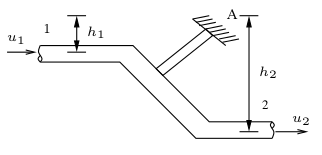
\includegraphics[width=0.5\linewidth]{TeX_files/chapter04-Dinamica/ejemplo1CMC}
		\end{center}
		
		
		Queremos calcular el momento sobre el punto A, usando el Volumen de
		Control mostrado en la siguiente figura.
		
		\begin{center}
			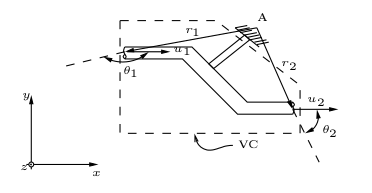
\includegraphics[width=0.5\linewidth]{TeX_files/chapter04-Dinamica/ejemplo1CMC1}
		\end{center}
		

		Suponemos que las propiedades del fluido (velocidad, densidad, presión)
		son uniformes en la entrada y en la salida, que el flujo es estacionario
		y que el peso del fluido y la tubería son menospreciables, asi como
		los efectos del rozamiento. Con estas hipótesis, la conservación del
		momento cinético es 
		\[
		\vec{M}_{T}=\vec{M}_{A}+\left[\vec{r}_{1}\times\left(-p_{1}\vec{S}_{1}\right)\right]+\left[\vec{r}_{2}\times\left(-p_{2}\vec{S}_{2}\right)\right]
		\]
		
		\[
		=\left(\vec{r}_{2}\times\vec{u}_{2}\right)\dot{m}_{2}-\left(\vec{r}_{1}\times\vec{u}_{1}\right)\dot{m}_{1}
		\]
		$\vec{M}_{A}$ es el momento realizado por la tubería \textbf{sobre}
		el fluido y transmitido a través del brazo al empotramiento en A.
		
		Dado que el flujo es unidimensional y los vectores de posición solo
		tienen componentes en $x$ y en $y$, los momentos son en la dirección
		$z$.

		Los módulos de los momentos que hacen las presiones son 
		\[
		\begin{cases}
			\left|\vec{r}_{1}\times\left(-p_{1}\vec{S}_{1}\right)\right| & =r_{1}p_{1}S_{1}\sin\theta_{1}=p_{1}S_{1}h_{1}\\
			\left|\vec{r}_{2}\times\left(-p_{2}\vec{S}_{2}\right)\right| & =-r_{2}p_{2}S_{2}\sin\theta_{2}=-p_{2}S_{2}h_{2}
		\end{cases}
		\]
		
		La variación de momento cinético del fluido es 
		\begin{align*}
			\left(\vec{r}_{2}\times\vec{u}_{2}\right)\dot{m}_{2}-\left(\vec{r}_{1}\times\vec{u}_{1}\right)\dot{m}_{1}=\left(r_{2}u_{2}\sin\theta_{2}-r_{1}u_{1}\sin\theta_{1}\right)\dot{m}\\
			\dot{m}=\left(h_{2}u_{2}-h_{1}u_{1}\right)
		\end{align*}
		
		Combinando todo, obtenemos $M_{A}$, 
		\[
		M_{A}=\left(h_{2}u_{2}-h_{1}u_{1}\right)\dot{m}-p_{1}S_{1}h_{1}+p_{2}S_{2}h_{2}
		\]
		\[
		=h_{2}\left(u_{2}\dot{m}+p_{2}S_{2}\right)-h_{1}\left(u_{1}\dot{m}+p_{1}S_{1}\right)
		\]
	
	\subsection*{Ejemplo 2:}
		Un irrigador por aspersion de radio $R$ da vueltas con una velocidad
		angular $\vec{\omega}=\omega\vec{k}$ y expulsa un caudal $Q$ por
		una tubería de sección $S$. El rozamiento sobre el eje es $\vec{M}_{r}=-M_{r}\vec{k}$.
		Queremos encontrar en el equilibrio una expresión para $\omega$.
		
		\begin{center}
			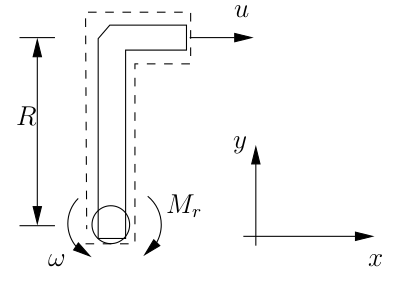
\includegraphics[width=0.5\linewidth]{TeX_files/chapter04-Dinamica/ejemplo2CMC}
		\end{center}
		
	

		Suponemos que el flujo es estacionario e incompresible, y que el peso
		del fluido y del irrigador son menospreciables. Despreciamos tambien
		los efectos de la fricción en el fluido. El brazo del irrigador no
		es estacionario, pero \textbf{sí} lo es el VC, de forma que la velocidad
		$u_{2}$ que pasa a través de la SC en la salida no es $u=\frac{Q}{S}$,
		sino 
		\[
		u_{2}=u-\omega R
		\]
		
		En el equilibrio, se cumple que 
		\[
		\vec{M}_{T}=-M_{r}\vec{k}=\left(\vec{r}_{2}\times\vec{u}_{2}\right)\dot{m}_{2}-\left(\vec{r}_{1}\times\vec{u}_{1}\right)\dot{m}_{1}
		\]
		Dado que $r_{1}=0$, tenemos $-M_{r}\vec{k}=\left(R\vec{\jmath}\times u_{2}\vec{\imath}\right)\dot{m}=-Ru_{2}\dot{m}\vec{k}$
		\begin{align*}
			M_{r}=\rho QR\left(u-\omega R\right)\\
			\omega=\frac{u}{R}-\frac{M_{r}}{\rho QR^{2}}=\frac{Q}{RS}-\frac{M_{r}}{\rho QR^{2}}
		\end{align*}

	
	\begin{itemize}
		\item \textbf{Sistema de referencia no inercial}
	\end{itemize}
	La única diferencia es que hay que añadir a los momentos realizados
	por las fuerzas externas, los momentos de las aceleraciones ficticias,
	
	\[
	\vec{M}_{T}-\int_{VC}\rho\left(\vec{r}_{0}\times\vec{a}'\right)\dif V=\int_{VC}\dparc{\left(\vec{r}_{0}\times\rho\vec{u}\right)}{t}\dif V+\oint_{SC}\left(\vec{r}_{0}\times\vec{u}\right)\rho\vec{u}\cdot\dif\vec{S}
	\]
	donde, tal y como vimos en el tema de conservación de la cantidad
	de movimiento, 
	\[
	\vec{a}'=\underbrace{\frac{\text{d}^{2}\vec{R}}{\text{d}t^{2}}}_{\text{ac. lineal del SR}}+\underbrace{\deriv{\vec{\Omega}}{t}\times\vec{r}}_{\text{ac. angular del SR}}+\underbrace{2\left(\vec{\Omega}\times\vec{u}\right)}_{\text{ac. de Coriolis}}+\underbrace{\vec{\Omega}\times\left(\vec{\Omega}\times\vec{r}\right)}_{\text{ac. centr\'ifuga}}
	\]
	
	
	\subsection*{Actividad 1:}
		
		Resolver el ejemplo 2, pero con un VC no inercial. 
		
		Ahora el VC rota solidario con el irrigador, con una velocidad angular
		$\omega$. Se debe obtener el mismo resultado.

\section{Las turbomáquinas hidráulicas}

Esta sección puede ser complementada con el capitulo 11 del libro de
White \cite{White2008}, o el 14 del de Çengel \cite{Cengel2014}. 


\subsection{La conservación del momento cinético y las turbomáquinas hidráulicas}

Las turbomáquinas hidráulicas se basan en la conservación del momento
cinético para transferir energia entre la máquina y el fluido. Estas
máquinas son: 
\begin{itemize}
	\item \textcolor{blue}{Bombas} (agua u otros líquidos) 
	\item \textcolor{blue}{Ventiladores} (aire) 
	\item \textcolor{blue}{Turbinas} (agua) 
\end{itemize}
En los dos primeros casos, la máquina transfiere momento cinético
y, por lo tanto, potencia al fluido. En el tercer caso, es el fluido
el que transfiere potencia a la máquina.

En todas estas máquinas el fluido es considerado incompresible.

Si el fluido es compresible, hablamos de \textbf{Turbomáquinas térmicas}
(compresores y turbinas de vapor). No serán tratadas en este curso.

Supongamos para simplificar la turbomáquina especificada en la figura.
La parte móvil donde realmente se tranfiere la energía recibe el nombre
de \textcolor{red}{rodete}. Está formado por una serie de \textcolor{red}{álabes}
que dirigen el fluido desde el interior hacia el exterior (bombas
y ventiladores centrífugos) o a la inversa (turbinas). En este caso,
los álabes son rectos. 

\begin{center}
	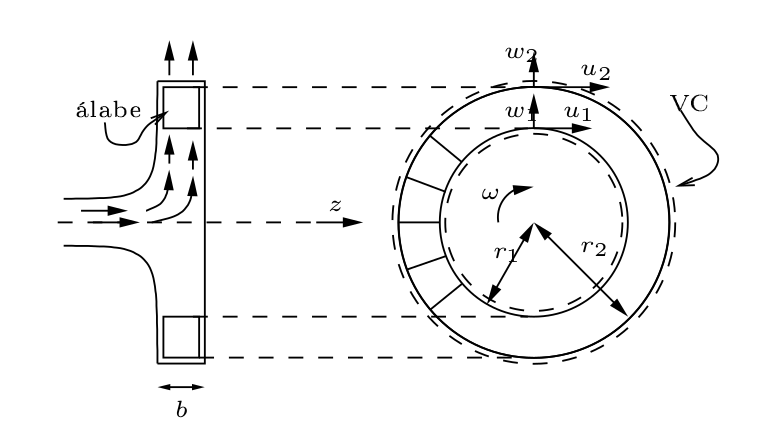
\includegraphics[width=0.5\linewidth]{TeX_files/chapter04-Dinamica/rodete1}
\end{center}

El fluido entra en el VC con una velocidad $\vec{c}_{1}=\vec{w}_{1}+\vec{u}_{1}$
y sale con una velocidad $\vec{c}_{2}=\vec{w}_{2}+\vec{u}_{2}$

Para mantener este flujo, debemos ejercer un momento mecánico sobre
el eje. Por la conservación del momento cinético, este momento será

\[
\vec{M}_{0}=\oint_{SC}\rho\left(\vec{r}\times\vec{c}\right)\vec{c}\cdot\dif\vec{S}=\rho Q\left[\left(\vec{r}_{2}\times\vec{c}_{2}\right)-\left(\vec{r}_{1}\times\vec{c}_{1}\right)\right]
\]

\[
M_{0}=\rho Q\left(r_{2}u_{2}-r_{1}u_{1}\right)
\]

Dado que $u_{1}=\omega r_{1}$ y $u_{2}=\omega r_{2}$, tenemos 
\[
M_{0}=\rho Q\omega\left(r_{2}^{2}-r_{1}^{2}\right)
\]
y la potencia requerida para bombear este fluido será 
\[
P=M_{0}\omega=\rho Q\omega^{2}\left(r_{2}^{2}-r_{1}^{2}\right)
\]


\subsection*{Actividad 1:}
	Realizar el cálculo de la potencia transmitida para un caudal de
	120 l/min de agua, una velocidad angular de 1725 rpm, unos diámetros
	del rodete de 15 cm y 25 cm y una anchura de rodete de 5 cm (constante).

\subsection{El triángulo de velocidades y la ecuación de Euler}


Las bombas, los ventiladores y las turbinas reales son algo más complicadas.
En realidad los álabes no son rectos, excepto para algunos ventiladores.

Centrándonos en el caso de las bombas centrífugas, los álabes suelen
estar inclinados hacia atrás según el sentido de giro. 

\begin{center}
	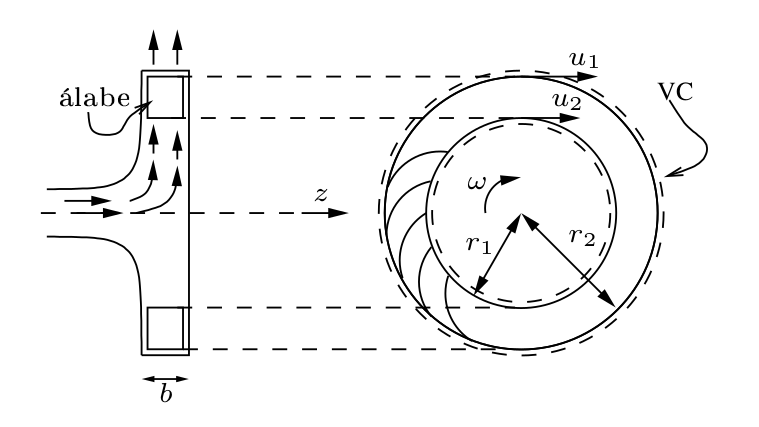
\includegraphics[width=0.5\linewidth]{TeX_files/chapter04-Dinamica/rodete2}
\end{center}


\begin{center}
	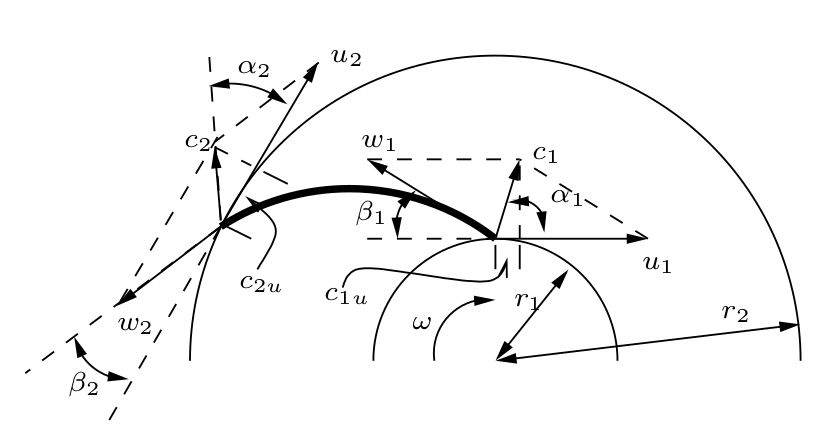
\includegraphics[width=0.5\linewidth]{TeX_files/chapter04-Dinamica/alabe1}
\end{center}

El momento cinético es transportado por la componente de la velocidad
$\vec{c}$ perpendicular al radio, es decir, $c_{1u}$ en la entrada
al VC y $c_{2u}$ en la salida. 

\begin{equation}
	M_{0}=\rho Q\left(r_{2}c_{2u}-r_{1}c_{1u}\right)
\end{equation}



Para calcular $c_{1u}$ y $c_{2u}$, se utilizan los \textcolor{red}{triángulos
de velocidades} 

\begin{center}
	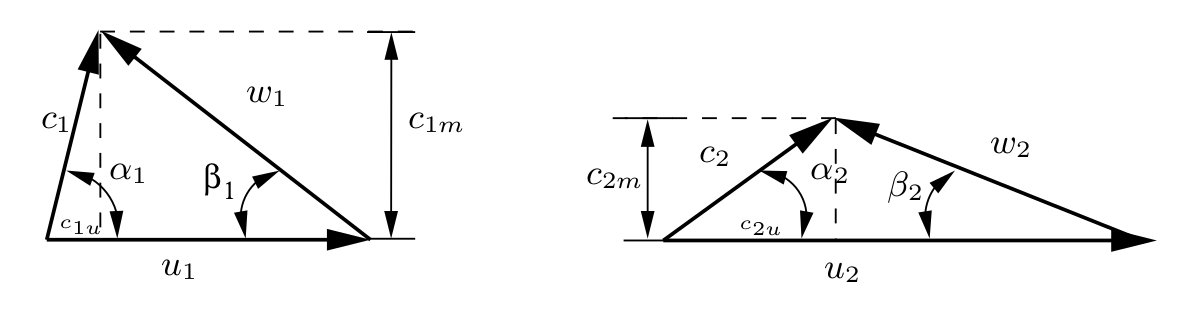
\includegraphics[width=0.7\linewidth]{TeX_files/chapter04-Dinamica/triangulo1}
\end{center}



\begin{equation}
	c_{1u}=u_{1}-\frac{c_{1m}}{\tan\beta_{1}}\qquad c_{2u}=u_{2}-\frac{c_{2m}}{\tan\beta_{2}}
\end{equation}
$c_{1m}$ y $c_{2m}$ se calculan a partir del caudal, 

\begin{equation}
	c_{1m}=\frac{Q}{S_{1}}=\frac{Q}{2\pi r_{1}b_{1}}\qquad c_{2m}=\frac{Q}{S_{2}}=\frac{Q}{2\pi r_{2}b_{2}}
\end{equation}

donde $b_{1}$ y $b_{2}$ son al ancho del rodete en la entrada y
en la salida.



La potencia necesaria para bombear el fluido es 

\begin{equation}
	P=M_{0}\omega=\rho Q\omega\left(r_{2}c_{2u}-r_{1}c_{1u}\right)=\rho Q\left(u_{2}c_{2u}-u_{1}c_{1u}\right)
\end{equation}

y la energia, en forma de altura de fluido, que transmite el rodete
al fluido es 

\begin{equation}
	\boxed{H_{t}=\frac{P}{\rho gQ}=\frac{1}{g}\left(u_{2}c_{2u}-u_{1}c_{1u}\right)}
\end{equation}


Esta es la \textcolor{red}{Ecuación de Euler} para Turbomáquinas,
y el subíndice $t$ indica que la expresión es teórica, ya que hay
muchos aspectos que no se han considerado: 
\begin{itemize}
	\item Número finito de álabes 
	\item Rozamiento en el flujo a través del rodete 
	\item Perfil de velocidad no uniforme en profundidad 
\end{itemize}


\subsection*{Actividad 2:}
	Repetir los cálculos de la Actividad 1, pero ahora los álabes no
	son rectos, sino que son tales que $\beta_{1}=35^{\circ}$ y $\beta_{2}=25^{\circ}$.
	Calcular la energía teórica que da el rodete, en forma de altura de
	fluido. 

\section{Ecuación integral de la conservación de la energía}

	
	Primera ley de la termodinámica para un sistema cerrado: 
	
	\begin{equation}
		\Deriv{E}{t}=\dot{Q}-\dot{W}
	\end{equation}
	
	
	\[
	\begin{array}{cc}
		\dot{Q} & \textrm{: calor transferido al sistema}\\
		\dot{W} & \textrm{: trabajo realizado por el sistema}
	\end{array}
	\]
	
	Aplicando el teorema del transporte de Reynolds al sistema:
	
	\[
	\Deriv{E}{t}=\int_{VC}\dparc{\rho e}{t}\text{d}V+\oint_{SC}\rho e\vec{u}\cdot\text{d}\vec{S}=\dot{Q}-\dot{W}
	\]
	
	donde 
	\[
	e=\underbrace{\frac{1}{2}u^{2}}_{\text{E. cinética}}+\underbrace{\phantom{\frac{1}{2}}gz\phantom{\frac{1}{2}}}_{\text{E. potencial}}+\underbrace{\phantom{\frac{1}{2}}\underline{u}\phantom{\frac{1}{2}}}_{\text{E. interna}}
	\]
	es la energía por unidad de masa.


\subsection{Análisis del trabajo}

	

	\begin{itemize}
		\item trabajo realizado por los esfuerzos normales: 
		\[
		\dot{W}_{n}=-\int_{SC}\tau_{nn}\vec{u}\cdot\text{d}\vec{S}\approx\int_{SC}p\vec{u}\cdot\text{d}\vec{S}
		\]
		
		\item trabajo realizado por los esfuerzos tangenciales: 
		\[
		\dot{W}_{t}=-\int_{SC}\vec{u}\cdot\underbrace{\left(\tens'\cdot\text{d}\vec{S}\right)}_{\vec{\tau}'\text{d}S}=-\int_{SC}\vec{u}\cdot\vec{\tau}'\text{d}S
		\]
		En general, se intenta escoger el $VC$ de forma que $\vec{u}\parallel\text{d}\vec{S}$,
		y, dado que $\vec{\tau}'$ está en $\text{d}S$, $\vec{v}\perp\vec{\tau}'$,
		y $\vec{v}\cdot\vec{\tau}'=0$ (flujos unidimensionales). 
		\item realizado por otros elementos externos, como, p.e., trabajo eléctrico,
		o trabajo mecánico de un eje (agitador, \ldots ). Lo expresamos como
		$\dot{W}_{e}$.
	\end{itemize}

	
	Para un Volumen de Control tal que $\vec{v}\Vert\text{d}\vec{S}$
	en las entradas y salidas, tendremos
	
	\[
	\dot{Q}-\dot{W}_{e}-\oint_{SC}p\vec{u}\cdot\text{d}\vec{S}=\int_{VC}\dparc{\rho e}{t}\text{d}V+\oint_{SC}\rho e\vec{u}\cdot\text{d}\vec{S}
	\]
	
	\[
	\Rightarrow\dot{Q}-\dot{W}_{e}=\int_{VC}\dparc{\rho e}{t}\text{d}V+\oint_{SC}\rho(e+\dfrac{p}{\rho})\vec{u}\cdot\text{d}\vec{S},
	\]
	
	Dado que $\underline{u}+\dfrac{p}{\rho}=h$, la conservación de la
	energía queda 
	

	\begin{equation}
		\boxed{\dot{Q}-\dot{W}_{e}=\int_{VC}\dparc{\rho e}{t}\text{d}V+\oint_{SC}\rho\left(h+gz+\frac{1}{2}u^{2}\right)\vec{u}\cdot\text{d}\vec{S}}
	\end{equation}
	
	
	\subsection*{Actividad 1:}
		¿Porqué no hemos incluido el trabajo realizado por la gravedad en
		$\dot{W}$?

\subsection*{Simplificaciones}
	
	\begin{itemize}
		\item \textcolor{blue}{Flujo permanente :} 
		\[
		\dparc{\rho e}{t}=0
		\]
		en todo el Volumen de Control 
		\item \textcolor{blue}{Propiedades constantes en las superficies de entrada
			(1) y de salida (2) (con flujo unidimensional)}: 
		\[
		\oint_{SC}\rho\left(h+gz+\frac{1}{2}u^{2}\right)\vec{u}\cdot\text{d}\vec{S}=
		\]
		\[
		\rho_{2}\left[h_{2}+gz_{2}+\frac{1}{2}u_{2}^{2}\right]u_{2}S_{2}-\rho_{1}\left[h_{1}+gz_{1}+\frac{1}{2}u_{1}^{2}\right]u_{1}S_{1}
		\]
		\[
		\boxed{\dot{Q}-\dot{W}_{e}=\rho_{2}\left[h_{2}+gz_{2}+\frac{1}{2}u_{2}^{2}\right]u_{2}S_{2}-\rho_{1}\left[h_{1}+gz_{1}+\frac{1}{2}u_{1}^{2}\right]u_{1}S_{1}}
		\]
	\end{itemize}

\subsection{Ecuación de Bernoulli}

	
	Flujo \textcolor{blue}{permanente},\textcolor{blue}{incompresible}
	y \textcolor{blue}{no viscoso}. $\dot{Q}=\dot{W}=0$
	
	\[
	\Rightarrow\rho_{2}\left[h_{2}+gz_{2}+\frac{1}{2}u_{2}^{2}\right]u_{2}S_{2}=\rho_{1}\left[h_{1}+gz_{1}+\frac{1}{2}u_{1}^{2}\right]u_{1}S_{1}
	\]
	
	Dado que $\rho_{2}u_{2}S_{2}=\rho_{1}u_{1}S_{1}=\dot{m}$, tenemos
	\[
	h_{2}+gz_{2}+\frac{1}{2}u_{2}^{2}=h_{1}+gz_{1}+\frac{1}{2}u_{1}^{2}
	\]
	
	Si suponemos también que no hay cambios en la energía interna, 
	\[
	\frac{p_{2}}{\rho}+gz_{2}+\frac{1}{2}u_{2}^{2}=\frac{p_{1}}{\rho}+gz_{1}+\frac{1}{2}u_{1}^{2},
	\]
	es decir, 
	
	\begin{equation}
		\frac{p}{\rho}+gz+\frac{1}{2}u^{2}=cte\quad\text{sobre una línea de corriente}
	\end{equation}
	
	
	Este es la conocida como \textcolor{red}{Ecuación de Bernoulli}.



	
	\subsection*{Actividad 2:}
		Una pareja que vive en una casa en la montaña decide aprovechar el
		arroyo de cerca de su casa para generar la energia necesaria para
		su vivienda. Compran una turbina en eBay y estiman que poniendo una
		presa podrían conseguir una altura en la entrada de la turbina de
		unos 4 metros. El caudal del arroyo es de unos 800 litros por segundo.
		Si en la salida de la turbina la velocidad del agua será de 3,6 m/s,
		estimad la potencia que podrían generar, menospreciando pérdidas por
		rozamiento.


\section{Ecuación diferencial de la conservación de la energía}

	
	$\vec{g}$ : fuerzas másicas
	
	Partiendo de la forma general de la conservación de la energia en
	un VC 
	\[
	\dot{Q}+\int_{VC}\vec{g}\cdot\vec{u}\rho\,\dif V+\oint_{SC}\vec{u}\cdot\left(\tens\cdot\dif\vec{S}\right)=\int_{VC}\dparc{\rho e}{t}\,\dif V+\oint_{SC}\rho e\vec{u}\cdot\dif\vec{S}
	\]
	donde $\tens$ incluye la diagonal y $e$ no incluye el término $gz$ 
	
	
	$\dot{Q}$ puede ser debido o bien a un flujo de calor ($\vec{q}$)
	a través de la $SC$ o bien a una producción de energía en el interior
	del $VC$ ($s$, que tiene unidades de W/kg). 
	\[
	\dot{Q=}-\oint_{SC}\vec{q}\cdot\dif\vec{S}+\int_{VC}s\rho\,\dif V
	\]
	

	
	Usando el Teorema de Gauss sobre las tres $SC$, queda 
	\begin{eqnarray*}
		-\int_{VC}\vec{\nabla}\vec{q}\dif V+\int_{VC}s\rho\,\dif V+\int_{VC}\vec{g}\cdot\vec{u}\rho\,\dif V+\int_{VC}\vec{\nabla}\left(\tens\cdot\vec{u}\right)\dif V=\\
		=\int_{VC}\dparc{\rho e}{t}\,\dif V+\int_{VC}\vec{\nabla}\cdot\left(\rho e\vec{u}\right)\dif V
	\end{eqnarray*}
	
	Si lo reescribimos en forma de componentes, usando el convenio de
	doble índice, y en una sola integral, obtenemos 
	\[
	\int_{VC}\left[-\dparc{q_{i}}{x_{i}}+\rho s+\rho g_{i}u_{i}+\dparc{\tau_{ij}u_{i}}{x_{j}}-\dparc{e\rho u_{i}}{x_{i}}+\dparc{\rho e}{t}\right]\dif V=0
	\]
	Dado que esto ha de ser cierto para todo $VC$, el integrando debe
	ser nulo, 
	\[
	-\dparc{q_{i}}{x_{i}}+\rho s+\rho g_{i}u_{i}+\dparc{\tau_{ij}u_{i}}{x_{j}}-\dparc{e\rho u_{i}}{x_{i}}+\dparc{\rho e}{t}=0
	\]
	

	
	Para simplificar esta expresión expandimos en primer lugar todas las
	derivadas, usando $e=\underline{u}+\frac{1}{2}u^{2}$. 
	\[
	-\dparc{q_{i}}{x_{i}}+\rho s+\rho g_{i}u_{i}+\tau_{ij}\dparc{u_{i}}{x_{j}}+u_{i}\dparc{\tau_{ij}}{x_{j}}=
	\]
	\[
	=\rho u_{i}\dparc{}{x_{i}}\left(\frac{u^{2}}{2}\right)+\frac{u^{2}}{2}\dparc{}{x_{i}}\left(\rho u_{i}\right)+\underline{u}\rho\dparc{u_{i}}{x_{i}}+\underline{u}u_{i}\dparc{\rho}{x_{i}}+\rho u_{i}\dparc{\underline{u}}{x_{i}}+
	\]
	\[
	+\rho\dparc{\phantom{}}{t}\left(\frac{u^{2}}{2}\right)+\left(\frac{u^{2}}{2}\right)\dparc{\rho}{t}+\underline{u}\dparc{\rho}{t}+\rho\dparc{\underline{u}}{t}
	\]
	

	
	Reordenando términos, tenemos 
	\[
	\underbrace{u_{i}\underbrace{\left[\dparc{\tau_{ij}}{x_{j}}+\rho g_{i}\right]}_{\rho\Deriv{u_{i}}{t}}}_{=\frac{\rho}{2}\Deriv{u^{2}}{t}}+\tau_{ij}\dparc{u_{i}}{x_{j}}-\dparc{q_{i}}{x_{i}}+\rho s=
	\]
	
	\[
	=\frac{\rho}{2}\underbrace{\left[\dparc{u^{2}}{t}+u_{i}\dparc{u^{2}}{x_{i}}\right]}_{=\Deriv{u^{2}}{t}}+\frac{u^{2}}{2}\underbrace{\left[\dparc{\rho u_{i}}{x_{i}}+\dparc{\rho}{t}\right]}_{=0}+\rho\underbrace{\left[\dparc{\underline{u}}{t}+v_{i}\dparc{\underline{u}}{x_{i}}\right]}_{\Deriv{\underline{u}}{t}}+
	\]
	
	\[
	+\underline{u}\underbrace{\left[\dparc{\rho}{t}+u_{i}\dparc{\rho}{x_{i}}\right]}_{\Deriv{\rho}{t}}+\underline{u}\rho\dparc{u_{i}}{x_{i}}
	\]
	
	
	\ldots{} y simplificando, 
	\[
	\tau_{ij}\dparc{u_{i}}{x_{j}}-\dparc{q_{i}}{x_{i}}+\rho s=\rho\Deriv{\underline{u}}{t}+\underline{u}\underbrace{\left[\Deriv{\rho}{t}+\rho\dparc{u_{i}}{x_{i}}\right]}_{=0}
	\]
	
	
	
	\begin{equation}
		\boxed{\tau_{ij}\dparc{u_{i}}{x_{j}}-\dparc{q_{i}}{x_{i}}+\rho s=\rho\Deriv{\underline{u}}{t}}
	\end{equation}
	
	
	
	Si ahora usamos la ley de Fourier 
	\[
	q_{i}=-k\dparc{T}{x_{i}}
	\]
	y la descomposición $\tau_{ij}=-p\delta_{ij}+\tau'_{ij}$, como hicimos
	con la conservación de cantidad de movimiento, 
	\[
	-p\dparc{u_{i}}{x_{j}}\delta_{ij}+\underbrace{\tau'_{ij}\dparc{u_{i}}{x_{j}}}_{\text{función disipación }\Phi}+\dparc{\phantom{}}{x_{i}}\left(k\dparc{T}{x_{i}}\right)+\rho s=\rho\Deriv{\underline{u}}{t}
	\]
	
	\begin{equation}
		\rho\Deriv{\underline{u}}{t}=\rho\left(\dparc{\underline{u}}{t}+u_{i}\dparc{\underline{u}}{x_{i}}\right)=-p\dparc{u_{i}}{x_{i}}+\Phi+\rho s+\dparc{\phantom{}}{x_{i}}\left(k\dparc{T}{x_{i}}\right)
	\end{equation}
	
	
	Para un fluido newtoniano, 
	\[
	\Phi=\mu\sum_{ij}\left(\dparc{u_{i}}{x_{j}}+\dparc{u_{j}}{x_{i}}\right)^{2}
	\]

\section{Derivación de la Ecuación de Bernoulli a partir de la Ecuación de Euler}
	
	Integramos la Ecuación de Euler 
	\[
	\rho\,\dparc{\vec{u}}{t}+\rho\left(\vec{u}\cdot\vec{\nabla}\right)\vec{u}=\rho\vec{g}-\vec{\nabla}p
	\]
	sobre una línea de corriente. La coordenada $s$ es la posición sobre
	la línea, y, dado que la velocidad debe ser tangente a la línea de
	corriente, sólo hay una ecuación de Euler para el módulo de $\vec{u}$,
	\[
	\dparc{u}{t}+u\dparc{u}{s}=-\frac{1}{\rho}\dparc{p}{s}-g\dparc{z}{s}
	\]
	
	Consideremos flujo estacionario, 
	\[
	u\dparc{u}{s}=-\frac{1}{\rho}\dparc{p}{s}-g\dparc{z}{s}
	\]
	
	
	Si una partícula de fluido se mueve una distancia $\dif s$ sobre
	la línea de corriente, tendremos 
	\begin{eqnarray*}
		\dparc{u}{s}\dif s & = & \dif u\\
		\dparc{p}{s}\dif s & = & \dif p\\
		\dparc{z}{s}\dif s & = & \dif z
	\end{eqnarray*}
	de forma que 
	\[
	u\dif u=-\frac{1}{\rho}\dif p-g\dif z\;\Rightarrow\;u\dif u+\frac{1}{\rho}\dif p+g\dif z=0
	\]
	\[
	\Rightarrow\;\frac{1}{2}u^{2}+\int\frac{\dif p}{\rho}+gz=\text{cte}
	\]
	y, si el fluido es incompresible, obtenemos la ecuación de Bernoulli
	\[
	\boxed{\frac{1}{2}u^{2}+\frac{p}{\rho}+gz=\text{cte}}
	\]
	


\section{Presión estática, dinámica y de remanso}

	
	Un \textcolor{red}{tubo de Pitot} es una sonda de diámetro muy pequeño,
	que se usa para medir la velocidad de un flujo. En la figura se muestra
	una en ángulo recto, usada para medir la velocidad en un canal. 
	
\begin{center}
	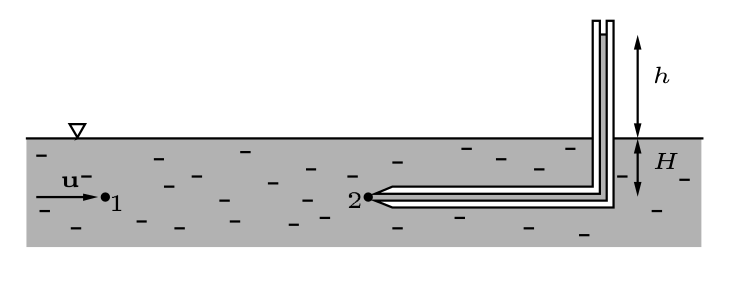
\includegraphics[width=0.5\linewidth]{TeX_files/chapter04-Dinamica/pitot1}
\end{center}

	
	
	El fluido penetra en la sonda y sube por el tubo hasta una altura
	$h$ por encima del nivel del canal. Esta altura es tal que la presión
	que crea en la boca del tubo contrarresta la energia que lleva el
	fluido. El punto 2, justo delante de la boca del tubo, recibe el nombre
	de \textcolor{green}{punto de estancamiento o de remanso}. En este
	punto, la velocidad del fluido es nula. El punto 1 está lo suficientemente
	lejos como para considerar que no está afectado por la sonda.
	
	Un tubo de Pitot mide la presión en el punto 2, es decir, la \textcolor{red}{presión
		de remanso} o \textcolor{red}{presión total}.
	
	Si aplicamos Bernoulli entre los puntos 1 y 2, que están en la misma
	línea de corriente, 
	\[
	\rho\,\frac{v_{1}^{2}}{2}+p_{1}=p_{2}=\rho g(H+h)
	\]
	
	Dado que $p_{1}=\rho gH$, obtenemos, de forma muy sencilla, 
	\[
	\frac{v_{1}^{2}}{2}=gh\;\Rightarrow\;v_{1}=v=\sqrt{2gh}
	\]
	
La presión total se compone de \textcolor{red}{presión estática} $p$
y \textcolor{red}{presión dinámica} $\frac{\rho v^{2}}{2}$. 

Con un tubo de Pitot podemos medir la presión dinámica y, por tanto,
la velocidad, si conocemos la presión estática (como era el caso del
canal abierto). 

Si no es el caso, utilizamos un \textcolor{green}{tubo de Pitot estático}
o \textcolor{green}{tubo de Prandtl}.

\begin{tabular}{cc}
	\begin{minipage}[c]{0.4\textwidth}%
		\begin{center}
			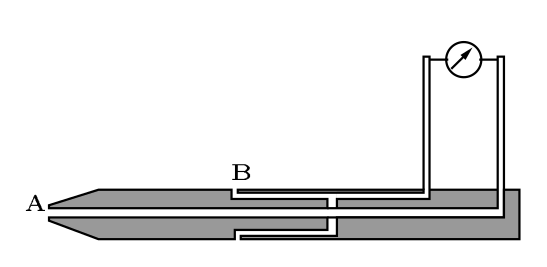
\includegraphics[width=0.7\linewidth]{TeX_files/chapter04-Dinamica/pitot2}
		\end{center}
		
		\[
		v=\sqrt{\frac{2(p_{A}-p_{B})}{\rho}}
		\]
		%
	\end{minipage} & %
	\begin{minipage}[c]{0.4\textwidth}%
		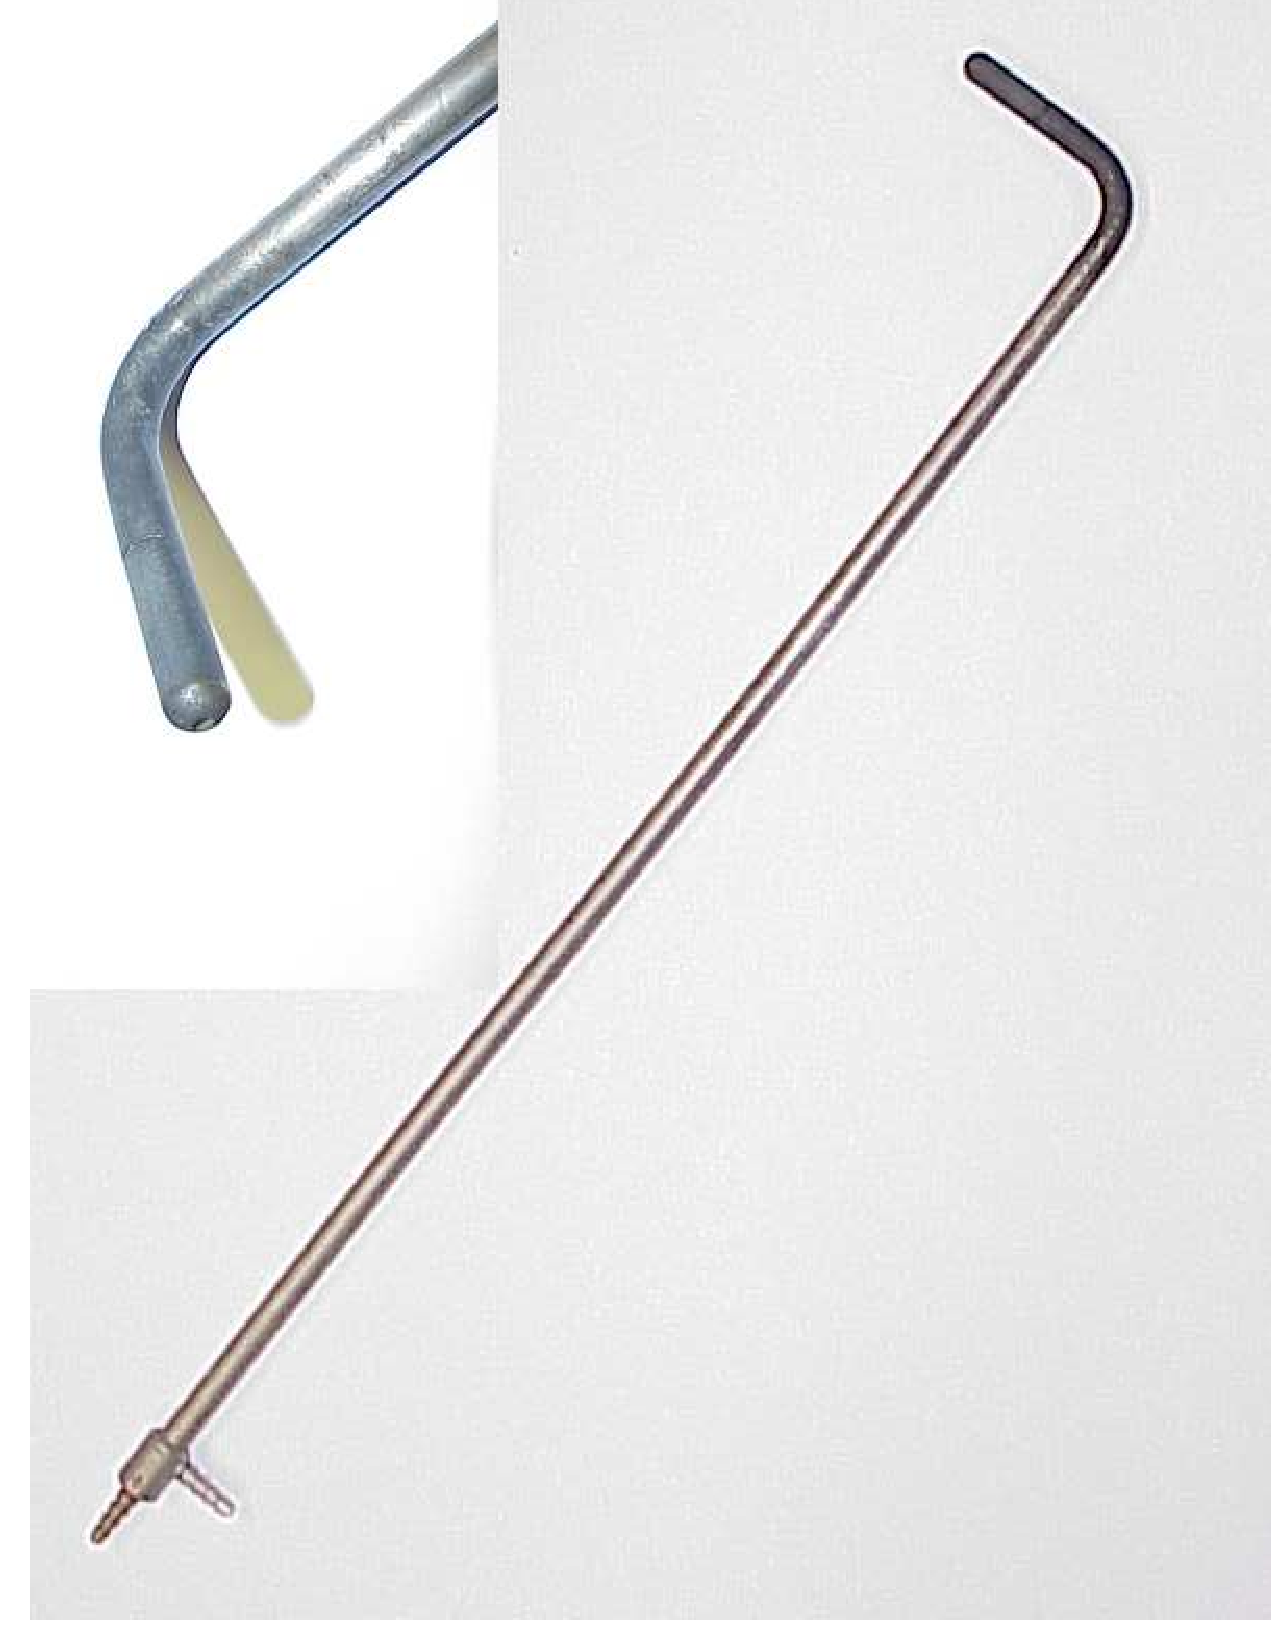
\includegraphics[clip,width=0.8\textwidth,angle=270]{TeX_files/chapter04-Dinamica/prandtl} %
	\end{minipage}\tabularnewline
\end{tabular}
\subsection{Tubo de Venturi}
	
	\begin{tabular}{cc}
		\begin{minipage}[c]{0.4\textwidth}%
			\begin{center}
				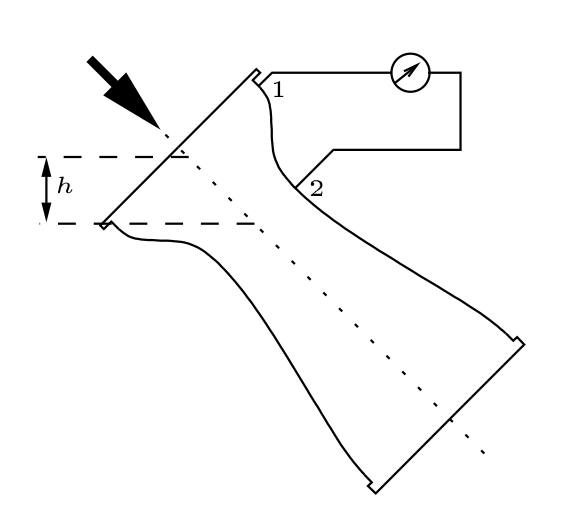
\includegraphics[width=\linewidth]{TeX_files/chapter04-Dinamica/venturi}
			\end{center}
		\end{minipage} & %
		\begin{minipage}[c]{0.4\textwidth}%
			
			\begin{align*}
				\frac{1}{2}\rho u_{1}^{2}+p_{1}+\rho gh=\frac{1}{2}\rho u_{2}^{2}+p_{2}\\
				\Rightarrow\frac{1}{2}\left(u_{2}^{2}-u_{1}^{2}\right)=\Delta p+\rho gh
			\end{align*}
			
			\[
			u_{1}=u_{2}\left(\frac{D_{2}}{D_{1}}\right)^{2}=u_{2}\beta^{2}
			\]
			
			\begin{align*}
				\frac{1}{2}\rho\left[1-\beta^{4}\right]u_{2}^{2}=\Delta p+\rho gh\\
				\Rightarrow\quad u_{2}=\sqrt{\frac{2\left(\Delta p+\rho gh\right)}{\rho\left[1-\beta^{4}\right]}}
			\end{align*}
			%
		\end{minipage}\tabularnewline
	\end{tabular}

	
	El caudal es $Q=u_{2}S_{2}$ . Éste caudal es teórico. El real se
	calcula multiplicando por un \textcolor{red}{coeficiente de descarga}
	$C_{d}$ que se obtiene por calibración. Normalmente $C_{d}\approx0.95\div1.0$.
	
	El caudal es, entonces, 
	\[
	Q_{r}=u_{2r}S_{2}=C_{d}S_{2}\sqrt{\frac{2\left(\Delta p+\rho gh\right)}{\rho\left[1-\beta^{4}\right]}}
	\]
	
	\subsection*{Actividad 1:}
		En un tubo de Venturi, de diámetros 200 mm y 160 mm, instalado horizontalmente,
		se mide una diferencia de presión de 25 mm de mercurio en una instalación
		de agua. ¿Cuál és el caudal teórico de agua que circula?

\subsection{Diafragma}
	
	La idea del diafragma es la misma que la del tubo de Venturi, pero
	carece de la sección de ampliación de la sección corriente abajo.
	Esto hace que el dispositivo sea más barato, y el montaje más sencillo.
	
	La ecuación para el caudal es la misma que para el tubo de Venturi,
	pero $C_{d}$ es generalmente menor. 
	
\begin{center}
	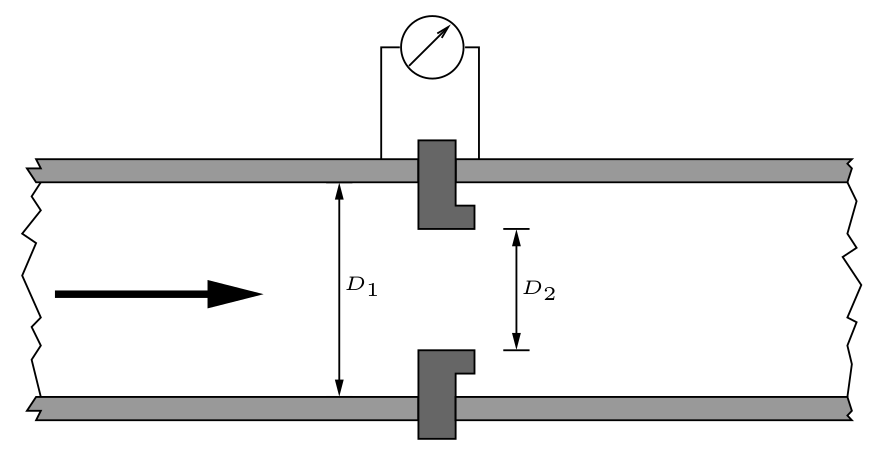
\includegraphics[width=0.7\linewidth]{TeX_files/chapter04-Dinamica/diafragma}
\end{center}

	


\subsection{Vaciado de un depósito}
	
	\begin{tabular}{cc}
		\begin{minipage}[c]{0.4\textwidth}%
			\begin{center}
				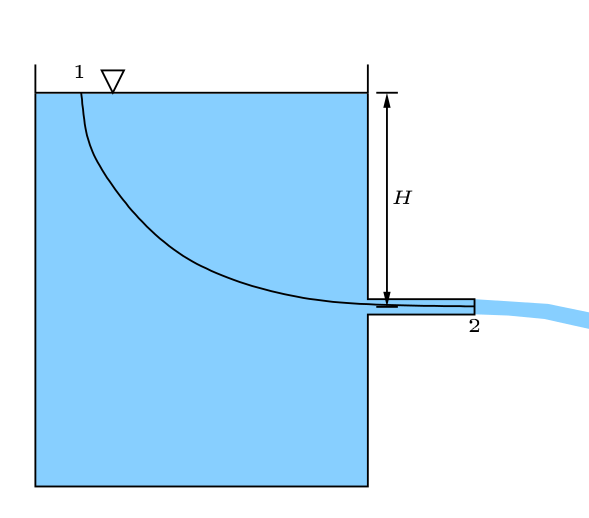
\includegraphics[width=\linewidth]{TeX_files/chapter04-Dinamica/deposito}
			\end{center}
		\end{minipage} & %
		\begin{minipage}[c]{0.5\textwidth}%
			Menospreciando la viscosidad, 
			\[
			\frac{1}{2}\rho u_{1}^{2}+p_{1}+\rho gH=\frac{1}{2}\rho u_{2}^{2}+p_{2}.
			\]
			
			Dado que tanto el punto 1 como el 2 están abiertos, $p_{1}=p_{2}=0$.
			Por otro lado, si suponemos que $S_{1}\gg S_{2}$, entonces $u_{1}^{2}\approx0$,
			\[
			\rho gH=\frac{1}{2}\rho u_{2}^{2}\;\Rightarrow\;\underbrace{u_{2}=\sqrt{2gH}}_{\text{Ec. de Torricelli}},
			\]
			y 
			\[
			Q_{t}=u_{2}S_{2}\sqrt{2gH}\qquad\text{(teórico)}
			\]
			%
		\end{minipage}\tabularnewline
	\end{tabular}
	
	\begin{tabular}{l>{\raggedright}p{0.7\textwidth}}
		\begin{minipage}[c]{0.4\textwidth}%
			\begin{center}
				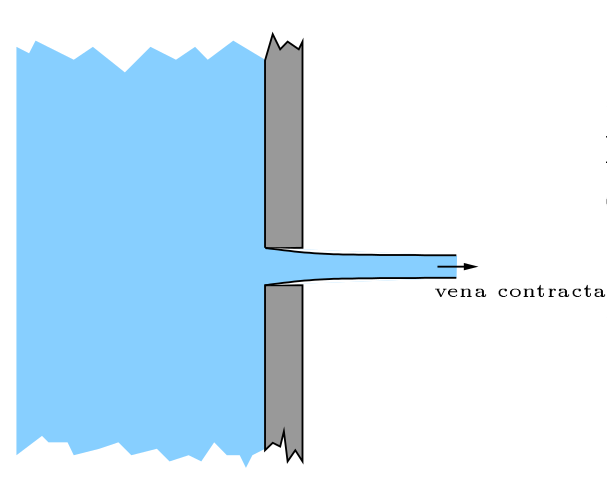
\includegraphics[width=\linewidth]{TeX_files/chapter04-Dinamica/orificio}
			\end{center}
		\end{minipage} & %
		\begin{minipage}[c]{0.6\textwidth}%
			Si la descarga se realiza a través de un orificio, se produce una
			vena contracta de forma que $S_{c}\lessapprox S_{2}$. 
			\[
			S_{c}=C_{c}S_{2}
			\]
			$C_{c}$ : \textcolor{blue}{Coeficiente de contracción} $\lessapprox1.0$
			
			Por otro lado, debido al rozamiento, la velocidad disminuye, 
			\[
			u_{c}=C_{v}u_{2}
			\]
			$C_{v}$ : \textcolor{blue}{Coeficiente de velocidad} $\lessapprox1.0$
			
			\begin{align*}
				Q=u_{c}S_{c}=C_{c}C_{v}S_{2}\sqrt{2gH}\\
				=C_{d}S_{2}\sqrt{2gH}
			\end{align*}
			$C_{d}$ : \textcolor{blue}{Coeficiente de descarga} %
		\end{minipage}\tabularnewline
	\end{tabular}

	
	\subsection*{Ejemplo: Cálculo de tiempo de vaciado de un depósito.}
		\[
		Q=C_{d}S_{2}\sqrt{\frac{2gH}{1-\left(\frac{S_{2}}{S_{1}}\right)^{2}}}=\frac{C_{d}S_{2}}{\sqrt{1-\left(\frac{S_{2}}{S_{1}}\right)^{2}}}\sqrt{2gH}
		\]
		\[
		u_{1}=\frac{Q}{S_{1}}=\frac{C_{d}\frac{S_{2}}{S_{1}}}{\sqrt{1-\left(\frac{S_{2}}{S_{1}}\right)^{2}}}\sqrt{2gH}=\underbrace{\frac{C_{d}\sqrt{2g}}{\sqrt{\left(\frac{S_{1}}{S_{2}}\right)^{2}-1}}}_{\alpha}\sqrt{H}
		\]
		\[
		u_{1}=-\deriv{H}{t}=\alpha H^{1/2}\Rightarrow\frac{\dif H}{H^{1/2}}=-\alpha\dif t\Rightarrow\int_{H_{0}}^{0}H^{-1/2}\dif H=-\alpha\int_{0}^{t}\dif t
		\]
		\[
		2\left.H^{1/2}\right]_{H_{0}}^{0}=-\alpha t\;\Rightarrow\;t=\frac{2}{\alpha}\sqrt{H}=\frac{2\sqrt{\left(\frac{S_{1}}{S_{2}}\right)^{2}-1}}{C_{d}\sqrt{2g}}\sqrt{H}
		\]

	
	\subsection*{Actividad 2:}
		Estima el tiempo que tarda en vaciarse una botella de agua de 1.5
		litros puesta boca abajo. ¿Porqué en realidad tarda mucho más?

	
	\subsection*{Actividad 3:}
		¿Cómo se modifican los cálculos si el depósito no es cilindrico (p.e.,
		un embudo)?

	

\backmatter
% bibliography, glossary and index would go here.

\end{document}